% ******************************* PhD Thesis Template **************************
% Please have a look at the README.md file for info on how to use the template

\documentclass[a4paper,12pt,custommargin,times,numbered,print,index]{PhDThesisPSnPDF}

% ******************************************************************************
% ******************************* Class Options ********************************
% *********************** See README for more details **************************
% ******************************************************************************

% `a4paper'(The University of Cambridge PhD thesis guidelines recommends a page
% size a4 - default option) or `a5paper': A5 Paper size is also allowed as per
% the Cambridge University Engineering Deparment guidelines for PhD thesis
%
% `11pt' or `12pt'(default): Font Size 10pt is NOT recommended by the University
% guidelines
%
% `oneside' or `twoside'(default): Printing double side (twoside) or single
% side.
%
% `print': Use `print' for print version with appropriate margins and page
% layout. Leaving the options field blank will activate Online version.
%
% `index': For index at the end of the thesis
%
% `draftclassic': For draft mode without loading any images (same as draft in book)
%
% `draft': Special draft mode with line numbers, images, and water mark with
% timestamp and custom text. Position of the text can also be modified.
%
% `abstract': To generate only the title page and abstract page with
% dissertation title and name, to submit to the Student Registry
%
% `chapter`: This option enables only the specified chapter and its references
%  Useful for review and corrections.
%
% ************************* Custom Page Margins ********************************
%
% `custommargin`: Use `custommargin' in options to activate custom page margins,
% which can be defined in the preamble.tex. Custom margin will override
% print/online margin setup.
%
% *********************** Choosing the Fonts in Class Options ******************
%
% `times' : Times font with math support. (The Cambridge University guidelines
% recommend using times)
%
% `fourier': Utopia Font with Fourier Math font (Font has to be installed)
%            It's a free font.
%
% `customfont': Use `customfont' option in the document class and load the
% package in the preamble.tex
%
% default or leave empty: `Latin Modern' font will be loaded.
%
% ********************** Choosing the Bibliography style ***********************
%
% `authoryear': For author-year citation eg., Krishna (2013)
%
% `numbered': (Default Option) For numbered and sorted citation e.g., [1,5,2]
%
% `custombib': Define your own bibliography style in the `preamble.tex' file.
%              `\RequirePackage[square, sort, numbers, authoryear]{natbib}'.
%              This can be also used to load biblatex instead of natbib
%              (See Preamble)
%
% **************************** Choosing the Page Style *************************
%
% `default (leave empty)': For Page Numbers in Header (Left Even, Right Odd) and
% Chapter Name in Header (Right Even) and Section Name (Left Odd). Blank Footer.
%
% `PageStyleI': Chapter Name next & Page Number on Even Side (Left Even).
% Section Name & Page Number in Header on Odd Side (Right Odd). Footer is empty.
%
% `PageStyleII': Chapter Name on Even Side (Left Even) in Header. Section Number
% and Section Name in Header on Odd Side (Right Odd). Page numbering in footer

% Uncomment to change page style
%\pagestyle{PageStyleII}

% ********************************** Preamble **********************************
% Preamble: Contains packages and user-defined commands and settings
% ******************************************************************************
% ****************************** Custom Margin *********************************

% Add `custommargin' in the document class options to use this section
% Set {innerside margin / outerside margin / topmargin / bottom margin}  and
% other page dimensions
\ifsetCustomMargin
  \RequirePackage[left=45mm,right=20mm,top=20mm,bottom=20mm]{geometry}
  \usepackage{fancyhdr}
  \fancyhf{} 
  \renewcommand{\headrulewidth}{0pt}
  \fancyfoot[C]{\thepage} % Page number in the center of the footer
  \pagestyle{fancy} 
\fi

% Add spaces between paragraphs
%\setlength{\parskip}{0.5em}
% Ragged bottom avoids extra whitespaces between paragraphs
\raggedbottom
% To remove the excess top spacing for enumeration, list and description
%\usepackage{enumitem}
%\setlist[enumerate,itemize,description]{topsep=0em}

% *****************************************************************************
% ******************* Fonts (like different typewriter fonts etc.)*************

% Add `customfont' in the document class option to use this section

\ifsetCustomFont
  % Set your custom font here and use `customfont' in options. Leave empty to
  % load computer modern font (default LaTeX font).
  %\RequirePackage{helvet}

  % For use with XeLaTeX
  %  \setmainfont[
  %    Path              = ./libertine/opentype/,
  %    Extension         = .otf,
  %    UprightFont = LinLibertine_R,
  %    BoldFont = LinLibertine_RZ, % Linux Libertine O Regular Semibold
  %    ItalicFont = LinLibertine_RI,
  %    BoldItalicFont = LinLibertine_RZI, % Linux Libertine O Regular Semibold Italic
  %  ]
  %  {libertine}
  %  % load font from system font
  %  \newfontfamily\libertinesystemfont{Linux Libertine O}
\fi

% *****************************************************************************
% **************************** Custom Packages ********************************

\RequirePackage{titlesec}

\newcommand{\PreContentTitleFormat}{\titleformat{\chapter}[display]{\bfseries\Large}
{\Huge{\chaptertitlename} \Huge\thechapter}
{1ex}{}
[\vspace{1ex}]}
\newcommand{\ContentTitleFormat}{\titleformat{\chapter}[display]{\normalfont\huge}
{\Large\filleft{\chaptertitlename} \Huge\thechapter}{1ex}
{\titlerule\vspace{1ex}\filright}
[\vspace{1ex}\titlerule]}
\newcommand{\PostContentTitleFormat}{\PreContentTitleFormat}
\PreContentTitleFormat

% Customize section titles to be bold and smaller
\titleformat{\section}
  {\bfseries\fontsize{14pt}{16pt}\selectfont} % Bold and smaller font for sections
  {\thesection} % Section numbering
  {1em} % Space between number and title
  {}

\titleformat{\subsection}
  {\bfseries\normalsize} % Bold and smaller font for subsections
  {\thesubsection} % Subsection numbering
  {1em} % Space between number and title
  {}

% ************************* Algorithms and Pseudocode **************************

%\usepackage{algpseudocode}


% ********************Captions and Hyperreferencing / URL **********************

% Captions: This makes captions of figures use a boldfaced small font.
%\RequirePackage[small,bf]{caption}

\RequirePackage[labelsep=space,tableposition=top]{caption}
\renewcommand{\figurename}{Fig.} %to support older versions of captions.sty


% *************************** Graphics and figures *****************************

%\usepackage{rotating}
%\usepackage{wrapfig}

% Uncomment the following two lines to force Latex to place the figure.
% Use [H] when including graphics. Note 'H' instead of 'h'
%\usepackage{float}
%\restylefloat{figure}

% Subcaption package is also available in the sty folder you can use that by
% uncommenting the following line
% This is for people stuck with older versions of texlive
%\usepackage{sty/caption/subcaption}
\usepackage{subcaption}

% ********************************** Tables ************************************
\usepackage{booktabs} % For professional looking tables
\usepackage{multirow}

%\usepackage{multicol}
%\usepackage{longtable}
%\usepackage{tabularx}


% *********************************** SI Units *********************************
\usepackage{siunitx} % use this package module for SI units
\usepackage{amssymb}

% ******************************* Line Spacing *********************************

% Choose linespacing as appropriate. Default is one-half line spacing as per the
% University guidelines

% \doublespacing
% \onehalfspacing
% \singlespacing

\setlength{\parindent}{0pt}
\setlength{\parskip}{1em} 

% ************************ Formatting / Footnote *******************************

% Don't break enumeration (etc.) across pages in an ugly manner (default 10000)
%\clubpenalty=500
%\widowpenalty=500

%\usepackage[perpage]{footmisc} %Range of footnote options


% *****************************************************************************
% *************************** Bibliography  and References ********************

%\usepackage{cleveref} %Referencing without need to explicitly state fig /table

% Add `custombib' in the document class option to use this section
\ifuseCustomBib
   \RequirePackage[numbers,sort&compress,authoryear]{natbib} % CustomBib

% If you would like to use biblatex for your reference management, as opposed to the default `natbibpackage` pass the option `custombib` in the document class. Comment out the previous line to make sure you don't load the natbib package. Uncomment the following lines and specify the location of references.bib file

%\RequirePackage[backend=biber, style=numeric-comp, citestyle=numeric, sorting=nty, natbib=true]{biblatex}
%\addbibresource{References/references} %Location of references.bib only for biblatex, Do not omit the .bib extension from the filename.

\fi

% changes the default name `Bibliography` -> `References'
\renewcommand{\bibname}{References}


% ******************************************************************************
% ************************* User Defined Commands ******************************
% ******************************************************************************

% *********** To change the name of Table of Contents / LOF and LOT ************

%\renewcommand{\contentsname}{My Table of Contents}
%\renewcommand{\listfigurename}{My List of Figures}
%\renewcommand{\listtablename}{My List of Tables}


% ********************** TOC depth and numbering depth *************************

\setcounter{secnumdepth}{2}
\setcounter{tocdepth}{2}


% ******************************* Nomenclature *********************************

% To change the name of the Nomenclature section, uncomment the following line

%\renewcommand{\nomname}{Symbols}


% ********************************* Appendix ***********************************

% The default value of both \appendixtocname and \appendixpagename is `Appendices'. These names can all be changed via:

%\renewcommand{\appendixtocname}{List of appendices}
%\renewcommand{\appendixname}{Appndx}
\usepackage{seqsplit}
\usepackage{array}
\usepackage{booktabs}
\usepackage{showframe}
\usepackage{textcomp}
\usepackage{sidecap}
\usepackage{caption}
\usepackage{multirow}
\usepackage{array}
\usepackage{booktabs}
\usepackage{makecell}
\usepackage{geometry}
\captionsetup[figure]{labelfont=bf, textfont=normalfont}
\captionsetup[table]{labelfont=bf, textfont=normalfont}

% *********************** Configure Draft Mode **********************************

% Uncomment to disable figures in `draft'
%\setkeys{Gin}{draft=true}  % set draft to false to enable figures in `draft'

% These options are active only during the draft mode
% Default text is "Draft"
%\SetDraftText{DRAFT}

% Default Watermark location is top. Location (top/bottom)
%\SetDraftWMPosition{bottom}

% Draft Version - default is v1.0
%\SetDraftVersion{v1.1}

% Draft Text grayscale value (should be between 0-black and 1-white)
% Default value is 0.75
%\SetDraftGrayScale{0.8}


% ******************************** Todo Notes **********************************
%% Uncomment the following lines to have todonotes.

%\ifsetDraft
%	\usepackage[colorinlistoftodos]{todonotes}
%	\newcommand{\mynote}[1]{\todo[author=kks32,size=\small,inline,color=green!40]{#1}}
%\else
%	\newcommand{\mynote}[1]{}
%	\newcommand{\listoftodos}{}
%\fi

% Example todo: \mynote{Hey! I have a note}

% ******************************** Highlighting Changes **********************************
%% Uncomment the following lines to be able to highlight text/modifications.
%\ifsetDraft
%  \usepackage{color, soul}
%  \newcommand{\hlc}[2][yellow]{{\sethlcolor{#1} \hl{#2}}}
%  \newcommand{\hlfix}[2]{\texthl{#1}\todo{#2}}
%\else
%  \newcommand{\hlc}[2]{}
%  \newcommand{\hlfix}[2]{}
%\fi

% Example highlight 1: \hlc{Text to be highlighted}
% Example highlight 2: \hlc[green]{Text to be highlighted in green colour}
% Example highlight 3: \hlfix{Original Text}{Fixed Text}

% *****************************************************************************
% ******************* Better enumeration my MB*************
\usepackage{enumitem}


% ************************ Thesis Information & Meta-data **********************
% Thesis title and author information, refernce file for biblatex
% ************************ Thesis Information & Meta-data **********************
%% The title of the thesis
\title{Investigating DNA methylation reprogramming in plant germlines}


%% Subtitle (Optional)
%\subtitle{}

%% The full name of the author
\author{Judit Tálas}

%% Department (eg. Department of Engineering, Maths, Physics)
\dept{
\makebox[\textwidth][c]{% 
\begin{minipage}{0.9\textwidth}
\centering 
Department of Cell and Developmental Biology
\newline
John Innes Centre
\end{minipage}%
}
\vspace{2em} % Adds vertical space after the department
}


%% Add extra vertical space after the department
% Adjust the value as needed

%% University and Crest
\university{University of East Anglia}
% Crest minimum should be 30mm.
%\crest{
\includegraphics[width=0.2\textwidth]{Figs/UEA_logo.pdf}}
%% Use this crest, if you are using the college crest
%% Crest long miminum should be 65mm
\crest{
\includegraphics[width=0.45\textwidth]{Figs/UEA_crest.png}}

%% College shield [optional] 
% Crest minimum should be 30mm.
%\collegeshield{
\includegraphics[width=0.45\textwidth]{Figs/Funders_logo.pdf}}


%% Supervisor (optional)
%% for multiple supervisors, append each supervisor with the \newline command
%\supervisor{Prof. A.B. Supervisor\newline
%Prof. C.D. Supervisor}

%% Supervisor Role (optional) - Supervisor (default) or advisor
% \supervisorrole{\textbf{Supervisors: }}
%% if no title is desired:
% \supervisorrole{}

%% Supervisor line width: required to align supervisors
%\supervisorlinewidth{0.35\textwidth}

%% Advisor (optional)
%% for multiple advisors, append each advisor with the \newline command
%\advisor{Dr. A. Advisor\newline
%Dr. B. Advisor}
     
%% Advisor Role (optional) - Advisor (default) or leave empty
% \advisorrole{Advisors: }
%% if no title is required
% \advisorrole{}

%% Advisor line width: required to align supervisors
%\advisorlinewidth{0.25\textwidth}


%% You can redefine the submission text:
% Default as per the University guidelines:
% ``This dissertation is submitted for the degree of''
\renewcommand{\submissiontext}{
\makebox[\textwidth][c]{% 
\begin{minipage}{0.9\textwidth} 
\centering 
\small 
This copy of the thesis has been supplied on condition that anyone who consults it is understood to recognise that its copyright rests with the author and that use of any information derived therefrom must be in accordance with current UK Copyright Law. In addition, any quotation or extract must include full attribution.
\vspace{2em}
\newline
\fontsize{14pt}{14pt}\selectfont 
This dissertation is submitted for the degree of
\vspace{1em}
\end{minipage}%
}
}

%% Full title of the Degree
\degreetitle{Doctor of Philosophy}

%% College affiliation (optional)
%\college{King's College}

%% Submission date
% Default is set as {\monthname[\the\month]\space\the\year}
%\degreedate{September 2014} 

%% Meta information
\subject{LaTeX} \keywords{{LaTeX} {PhD Thesis} {Biology} {University of
East Anglia}}


% ***************************** Abstract Separate ******************************
% To printout only the titlepage and the abstract with the PhD title and the
% author name for submission to the Student Registry, use the `abstract' option in
% the document class.

\ifdefineAbstract
 \pagestyle{empty}
 \includeonly{Declaration/declaration, Abstract/abstract}
\fi

% ***************************** Chapter Mode ***********************************
% The chapter mode allows user to only print particular chapters with references
% Title, Contents, Frontmatter are disabled by default
% Useful option to review a particular chapter or to send it to supervisior.
% To use choose `chapter' option in the document class

\ifdefineChapter
 \includeonly{Chapter1/chapter1}
\fi

% ******************************** Front Matter ********************************
\begin{document}

\mainmatter

\maketitle

% ******************************* Thesis Declaration ***************************

\begin{declaration}

Throughout this thesis, I present both my original work and contributions from others. Where data from other sources is included, appropriate references are provided. A summary of the lines and libraries, either generated by myself and colleagues in the lab or sourced from published literature, can be found in Tables \ref{ch2:workbyothers} and \ref{ch3:workbyothers}.

\end{declaration}


% ************************** Thesis Acknowledgements **************************

\begin{acknowledgements}      

Throughout the process of writing this thesis I had the opportunity to reflect on these last 4 years and how thankful and privileged I am for having the people around me that made this all possible. First, I would like to thank the John Innes Centre and the NRPDTP programme for providing the perfect environment to carry out this research. I felt so spoilt by all the support and guidance offered by Lab Support, Bioimaging, Horticultural Sevices and Research Computing, thank you all!

I want to thank Christine Faulkner for offering insightful, impartial feedback on my PhD, whilst also being encouraging, realistic and empathetic. To my supervisor Xiaoqi Feng - thank you for always sharing my excitement for my project, allowing me to take the reign in exploring topics that excited me and for your unwavering faith in my abilities, both personal and scientific. 

I am also deeply grateful to the members of the Feng lab, past and present from whom I've have learnt so much. To the lovely postdocs Yalin and Shaoli, it was so much fun to work with you and your work ethic and enthusiasm never fails to impress me. A big thank you to Shujuan an Chris, who always looked out for me after the lab moved abroad, your presence in the lab made all the difference. You were both always so approachable, easygoing and were always up for helping me or just having a much needed pep talk or chat. I owe a special thanks to Jincheng Long who taught me everything I know about sRNAs and techniques in the lab - you were an amazing mentor in my first two years and so much fun to be around!  I also want to thank Martin Vickers for making bioinformatics approachable and enjoyable — it became the highlight of my PhD thanks to you.

To my adoptive lab, the Carella Lab -  Hetty, Hyeonmin, Bea, Ellie, Sam and Kayla - you are all amazing! You made me feel so welcome in the lab and I will miss our lunches and silly (and serious) conversations. I owe a massive thanks to Phil Carella - thank you so much for agreeing to be my supervisor for the final part of my PhD. Your kindness, support, and calm presence made all the difference. I honestly couldn’t have completed this PhD without you.

I want to thank my friends, Sophie, Deirdre, Cat, Joe and especially Emily, you have been there through the ups and downs of these four years, I feel so privileged to have found friends like you. Your kindness, humour, enthusiasm and infectious passion for science has made living in Norwich around you amazing. I will miss our dinner parties, coffees and hangouts so much. I’m so proud of all of you for reaching the end of your PhDs!

Köszönöm a családomnak: Papa, Mama, Andris, Zsófi, Zsuzsi, Bogesz, Dorka, Balu, Zsuzsa, Nagyi és Nagypapa köszönöm a sok segítséget, bíztatást és támogatást, nélkületek nem sikerült volna! Nagyon szeretlek titeket!

To Johnny, thank you for being my cheerleader, you have been the most important rock throughout these 4 years. Thank you for believing in me and for moving to Norwich so I could continue to pursue this degree. Thank you for cooking for me, and offering distractions when I needed them most.

Lastly, I want to give a huge thank you to Jimmy. You have been the most amazing, patient and invaluable mentor and friend throughout my PhD. The amount of dedication, kindness and enthusiasm you showed towards my project is absolutely incredible, even after you moved away to the other side of the pond. I am so grateful for your guidance and friendship. You made it possible for me to see this project through, and I truly couldn’t have completed this degree without you.

Thank you all!


\end{acknowledgements}

% ************************** Thesis Abstract *****************************

\begin{abstract}

Epigenetic reprogramming is an essential part of reproduction across both animal and plant kingdoms. Although the two kingdoms have diverged more than 1.5 billion years ago, they both have convergently evolved systems that protect the integrity of the genome throughout generations. This is in part due to the threat of mobile transposable elements, which when uncontrolled can lead to genomic instability through insertions and rearrangements. Whilst animals reset DNA methylation during germline development, plants largely maintain symmetric CG and CHG DNA methylation. However, asymmetric CHH methylation undergoes tightly regulated reprogramming during male sexual lineage development in plants.

This thesis investigates the dynamics of epigenetic regulation during plant reproduction in two distinct systems: \textit{Arabidopsis thaliana} and \textit{Marchantia polymorpha}. In \textit{Arabidopsis}, the expression patterns of key RNA-directed DNA methylation (RdDM) components was examined, alongside exploring the small RNA (sRNA) profiles post-meiosis during the development of the male sexual lineage. The results reveal a complex spatiotemporal regulation of RdDM factors and a shift away from CLSY-dependent sRNA biogenesis after meiosis, potentially involving non-canonical RdDM pathways.

In the basal land plant \textit{Marchantia polymorpha}, recent studies have revealed the presence of N4-methylcytosine (4mC) in the male germline, an epigenetic modification previously thought to exist only in prokaryotes. During spermiogenesis, 4mC is deposited globally at CG sites, yet after fertilisation, the mature embryo loses this mark, and the knockout of 4mC leads to accelerated embryonic development. This study further explores the fate of paternal 4mC in early \textit{Marchantia} embryos and provides evidence that 4mC is actively removed before pronuclear fusion. Further investigation reveals that the loss of 4mC accelerates the onset of the first nuclear division and imposes a partial fertility cost, ultimately impacting long-term embryonic development.

\end{abstract}



% *********************** Adding TOC and List of Figures ***********************

\tableofcontents

%\listoffigures

%\listoftables

% \printnomenclature[space] space can be set as 2em between symbol and description
%\printnomenclature[3em]

%\printnomenclature

% ******************************** Main Matter *********************************
%\mainmatter

%!TEX root = ../thesis.tex
%*******************************************************************************
%*********************************** First Chapter *****************************
%*******************************************************************************

\chapter{Introduction}  %Title of the First Chapter

\ifpdf
    \graphicspath{{Chapter1/Figs/Raster/}{Chapter1/Figs/PDF/}{Chapter1/Figs/}}
\else
    \graphicspath{{Chapter1/Figs/Vector/}{Chapter1/Figs/}}
\fi


\section{Introduction to epigenetics in prokaryotes, animals, and plants } %Section - 1.1 

Epigenetics refers to a “stably heritable phenotype resulting from changes in a chromosome without alterations in the DNA sequence” \cite{RN135}. In eukaryotic organisms, chromatin organisation plays a critical role in various cellular processes, including differentiation, development, response to environmental stimuli, and the maintenance of genome integrity. Chromatin consists of DNA and specialised proteins called histones, which together form nucleosomes. Histones exist in multiple variants and can undergo various modifications that influence chromatin structure, accessibility, and gene expression \cite{RN289,RN284}. The addition of a methyl group to the 5th carbon of cytosine results 5-methylcytosine (5mC) which is an example of DNA methylation - another epigenetic modification. In prokaryotic organisms, DNA methylation was originally identified as a component in the restriction-modification pathway wherein methylated sequences are recognised as self, and unmethylated sequences are targeted for cleavage by restriction enzymes, thus safeguarding the genome against invading unmethylated phage DNA \cite{RN96,RN95}.

In eukaryotic systems, including plants and animals, DNA methylation functions oppositely: invading transposable elements (TEs) are silenced by DNA methylation. In plants, 5mC is the most prevalent form of DNA methylation, primarily occurring in heterochromatic regions, though methylated loci can also be found in genic regions \cite{RN228,RN193}. DNA methylation can directly suppress transcription and gene expression by hindering the binding of transcription factors \cite{RN290}. One of the earliest evidences for epigenetic modifications in plants was discovered in the \textit{Arabidopsis thaliana} gene \textit{SUPERMAN} (\textit{SUP}). Mutations in \textit{SUPERMAN} affect normal floral development. Interestingly, some alleles exhibited the mutant phenotype without any alterations in the DNA sequence. The \textit{clark kent} epialleles were uncovered when it was discovered that the promoter sequence of \textit{SUP} was methylated. In addition, SUP expression correlates with the extent of \textit{SUP} promoter methylation \cite{RN100}. This discovery was among the first to highlight the role of DNA methylation in controlling transcriptional expression in plants. Since then, the field of plant epigenetics has significantly expanded, uncovering a myriad of complex mechanisms by which DNA methylation and other epigenetic modifications regulate gene expression, development and protect genome integrity throughout generations.

\section{Transposable elements}

The size of different plant genomes is highly variable and not necessarily related to their complexity. Among eukaryotes, flowering plants display the most extreme genome size variation, with differences of up to 2400-fold; for instance, the genome of \textit{Genlisea aurea} is just 63.6 megabases (Mb), while that of \textit{Paris japonica} reaches a staggering 150 gigabases (Gb) \cite{RN76,RN81}. TEs, which are selfish and repetitive DNA sequences, persist in genomes by copying and inserting themselves into various genomic locations \cite{RN102}. TEs are also essential for driving genome evolution: they can regulate gene expression, unequal crossover, recombination rate and in general contribute to genomic variation \cite{RN103}. TEs have had some prominent stabilising impacts on  chromosomes, playing a vital role in the evolution  of repetitive structures including the centromere  and telomeres \cite{RN101}.

However, the majority of TE activity tends to be harmful, posing risks to genome integrity and often being disadvantageous to the organism \cite{RN103}. Transposable elements can cause heritable disruption to a vast range of cellular functions by insertion into promoter, regulatory or genic regions. For example, the mobilisation of the \textit{CAC1} TE results in the disruption of the \textit{DWARF4}  gene and severe growth defects in \textit{Arabidopsis} \cite{RN105}.

TEs are categorized into two classes: Class I (retrotransposons) and Class II (DNA transposons) TEs. Class I TEs are transcribed via an RNA intermediate, which then undergoes reverse transcription before insertion at another site in the genome. The reverse transcriptase required for this process is usually encoded within the transposable element itself. One of the largest families of Class I TEs are long-terminal-repeat (LTR) retrotransposons. Some of these LTRs (flanking the TE) have acquired transfer-RNA (tRNA) fragments, which can be used as binding sites for host tRNAs. Subsequently, the clover leaf structure of the tRNA can be recognised as a primer to initiate reverse transcription and transposition. To combat this, some hosts cleave tRNAs into tRNA fragments (tRFs) that compete for these LTR binding sites, thereby silencing these retrotransposons \cite{RN66,RN67,RN68}.

Conversely, Class II TEs encode transposase enzymes that excise the DNA segments and insert them elsewhere in the genome.  Both Class I and Class II TEs can be further classified as either autonomous or non-autonomous elements. Autonomous elements encode all the necessary machinery for their own mobilisation, whereas non-autonomous elements lack some or all of these factors and rely on trans-acting transposases to facilitate their transposition \cite{RN106,RN107}.

In addition to disrupting the function of individual genes, the excision and insertion of TEs can destabilise genome structure \cite{RN103}. The repetitive nature of TEs can cause non-allelic homologous recombination during meiosis, leading to reproductive defects and the formation of dicentric or acentric chromosomes \cite{RN108}. 

The contribution of TEs to genome size varies massively: while they comprise only around 21\% of the \textit{Arabidopsis} genome \cite{RN109},  crops with larger genomes have gone through significant TE amplification typically dominated by a few TE families \cite{RN110,RN113}, resulting in an 82\% and 85\% genomic TE content of wheat and maize respectively \cite{RN110,RN111}. The importance of TEs in genome regulation is further exemplified in maize, where disruption of DDM1, a key chromatin remodeler required for the genome-wide maintenance of DNA methylation, results in embryo lethality \cite{RN112}. Thus, whilst mutations of the components of the pathway for establishment and maintenance of DNA methylation have no apparent phenotypic effects in \textit{Arabidopsis}, it offers an important model system for exploring the underlying mechanisms of genome-wide epigenetic regulation.

\section{Chromatin Structure}

The regulation of gene and TE transcription is essential for both prokaryotic and eukaryotic organisms. In eukaryotes, DNA is organised into chromatin, with the nucleosome serving as the basic unit. In a nucleosome, DNA is wrapped around histone octamers, which consist of two H2A-H2B heterodimers and one H3-H4 heterotetramer, along with the linker histone H1, altogether encompassing 147 base pairs of DNA \cite{RN294}. Nucleosomes are further organised into dynamic higher-order chromatin structures, which mediate chromatin accessibility and arrange the genome into more open, gene-rich euchromatic regions and more condensed heterochromatic regions, typically located around chromosome ends or pericentromeric regions in \textit{Arabidopsis} \cite{RN299}. 

Chromatin structure is regulated through histone modifications, such as acetylation, methylation, phosphorylation, or ubiquitination, which convey chromatin states and interact with various pathways that promote or repress chromatin accessibility and condensation.  For instance, trimethylation of lysine 27 of histone H3 (H3K27me3) and di- or trimethylation of lysine 9 on histone H3 (H3K9me2 or H3K9me3) are associated with repressed chromatin states. In contrast, H3K27 acetylation (H3K27ac) is associated with active promoters, as is histone H3 lysine 4 trimethylation (H3K4me3). Additionally, trimethylation of lysine 36 on histone H3 (H3K36me3) is correlated with active transcription in gene bodies \cite{RN297,RN298}. 

There are also specific histone variants that are either highly conserved across eukaryotes or unique to particular systems. For instance, H2A.Z is conserved across eukaryotes and is enriched in euchromatic regions, where it facilitates the recruitment of RNA Polymerase II in yeast, plants, and animals \cite{RN295,RN296}. In contrast, H2B.8 is specific to the sperm cells of \textit{Arabidopsis} and plays a key role in mediating sperm chromatin condensation \cite{RN285}.

\section{DNA methylation maintenance and the RdDM pathway} 

The existence of epigenetic marks implies that there are mechanisms to read, write and erase them. Cytosine methylation exists in one of three sequence contexts: the symmetric CG and CHG and the asymmetric CHH (where H = A, T or C).  This contrasts with mammals, in  which most methylation is directed to CG sites  and is not inherited by the next generation \cite{RN228}. 

\begin{figure}[htbp!] 
\centering    
    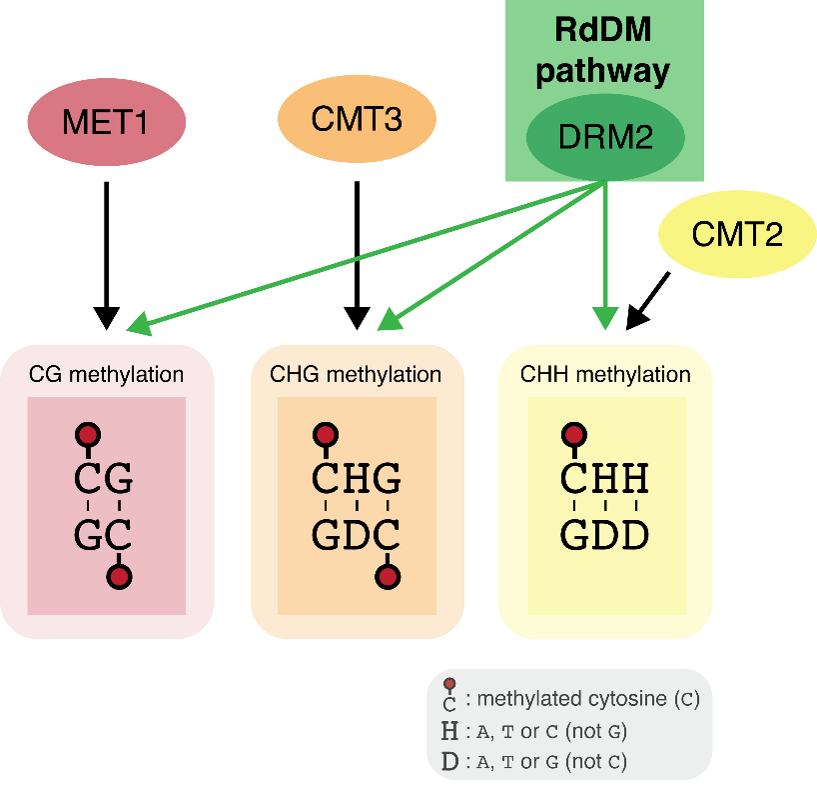
\includegraphics[width=0.5\textwidth]{Chapter1/Figs/base_mods.png}
\caption{DNA methylation sequence contexts and their associated DNA methyltransferases (Figure from \cite{RN61})}
\label{fig:meth_pathways}
\captionsetup{font=small}
    \caption*{}
\end{figure}

RNA-directed DNA methylation (RdDM) is a pathway that can methylate cytosine in any sequence context \cite{RN33}. In plants, it is also the only pathway responsible for the \textit{de novo} methylation of previously unmethylated regions. During DNA replication, modifications at symmetric CG and CHG sites result in a hemimethylated state, where only one strand of the daughter DNA retains methylation. Full methylation can be restored by the highly conserved maintenance methyltransferases METHYLTRANSFERASE 1 (MET1, a homolog of DNMT1) and CHROMOMETHYLASE 3 (CMT3) (Figure \ref{fig:meth_pathways}) \cite{RN61}. CHH sites are maintained by CMT2, however, due to the asymmetry of CHH methylation, methylation information may be lost during replication, necessitating the recruitment of RdDM for both \textit{de novo} methylation and maintenance. Therefore, to sustainably combat the detrimental effects of TE mobilisation, plants have evolved ways to keep transposon activity tightly controlled through RdDM. Additionally, the robustness of the system is enhanced by the fact that CMT2/3 and SET domain histone methyltransferases (KYP, SUVH5/6) maintain non-CG methylation and H3K9me2 in an interdependent manner. Specifically, the chromo and BAH domains of CMT3 interact directly with H3K9me2, allowing it to recognise other heterochromatic marks and establish a positive feedback loop \cite{RN33}.

Following the sequencing of the \textit{Arabidopsis} genome, two unexpected variants of RNA Polymerase II were discovered: RNA Polymerase IV (Pol IV) and RNA Polymerase V (Pol V) \cite{RN115}. Through these two variants, the RdDM pathway generates small RNAs (sRNAs) in heterochromatic regions and is able to target \textit{de novo} DNA methylation to these regions. The Pol IV-associated pathway initiates through recruitment via H3K9me2 associated chromatin remodeller SAWADEE HOMEODOMAIN HOMOLOG 1 (SHH1) \cite{RN206,RN98,RN99,RN116}.  Pol IV works in concert with chromatin remodellers CLASSY 1-4 (CLSY 1-4) to transcribe a short single-stranded RNA precursor \cite{RN117}, which is then extended into double-stranded RNA by RNA-dependent RNA polymerase 2 or 6 (RDR2 or RDR6) \cite{RN61,RN33}. This double-stranded RNA is processed by DICER-LIKE 3 (DCL3) into 24-nucleotide small interfering RNAs (24nt siRNAs), which are subsequently loaded onto specific ARGONAUTE proteins (AGO4/5/6/9) \cite{RN33} (Figure \ref{fig:RdDM_overview}). This complex interplay between DNA methylation and histone modifications ensures that patterns of DNA methylation are stably inherited through mitosis, maintaining consistent gene expression and genome stability across cell divisions.

\begin{figure}[htbp!] 
\centering    
    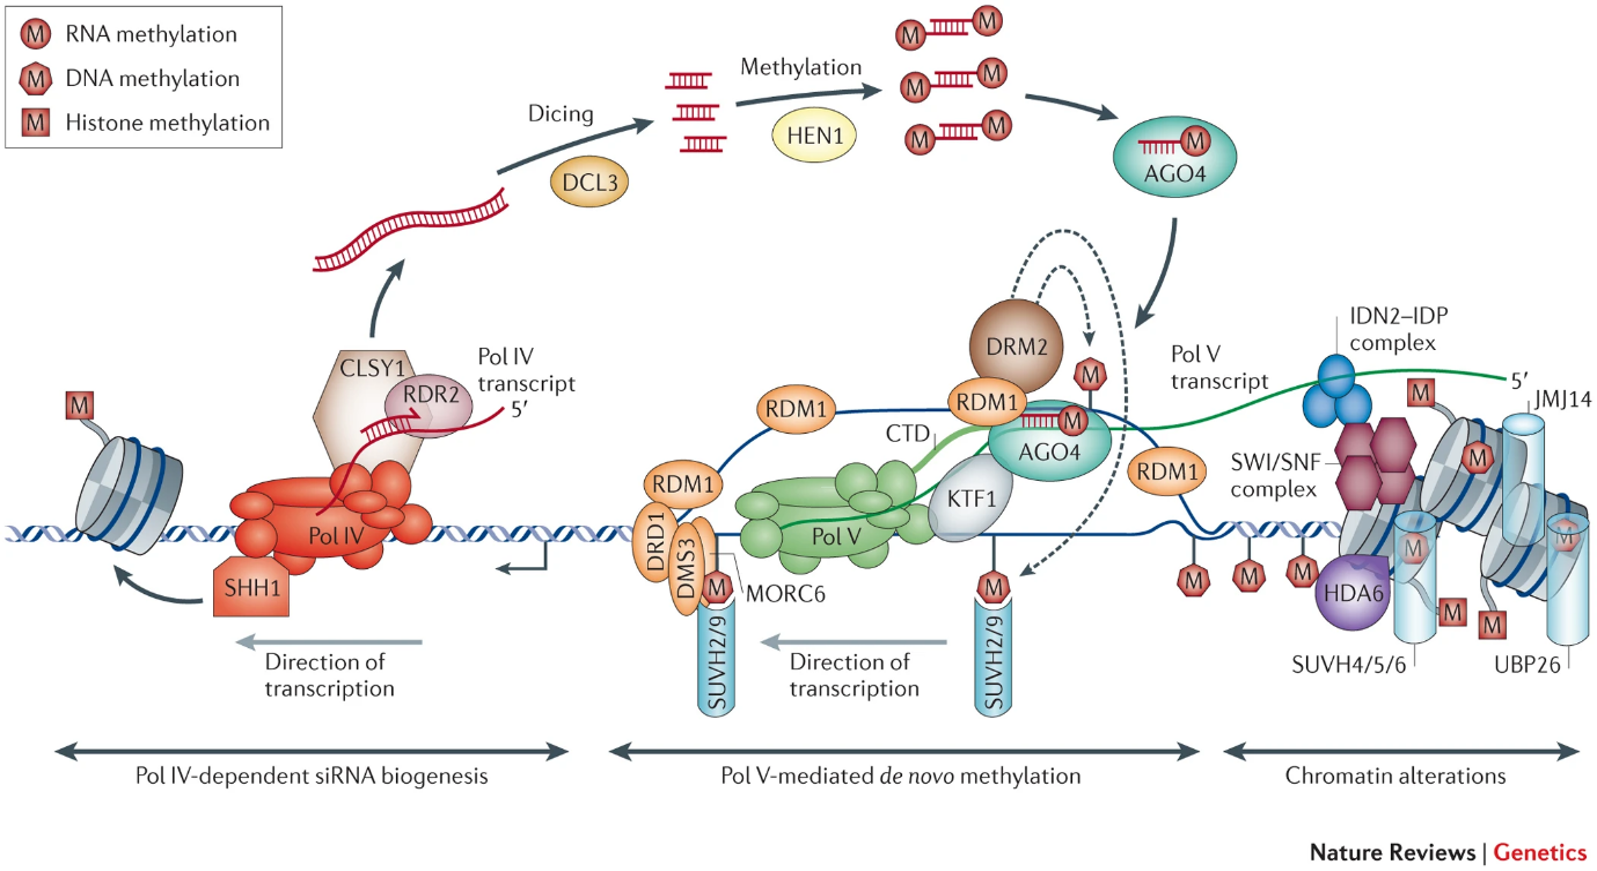
\includegraphics[width=1\textwidth]{Chapter1/Figs/RdDM.png}
\caption{An overview of the canonical RdDM pathway (Figure from \cite{RN33})}
\label{fig:RdDM_overview}
\captionsetup{font=small}
    \caption*{}
\end{figure}

Independently, Pol V is recruited by the DDR complex composed of chromatin remodellers DEFECTIVE IN MERISTEM SILENCING 3 (DMS3), DEFECTIVE IN RNA-DIRECTED DNA METHYLATION 1 (DRD1) and RNA-DIRECTED DNA METHYLATION (RDM1), along with SUPPRESSOR OF VARIEGATION 3–9 HOMOLOG 4/5/6 (SUVH4/5/6) methyl-DNA-binding proteins. The Pol V complex transcribes a single stranded RNA scaffold \cite{RN33}. The siRNA-AGO complex binds to this complementary scaffold RNA, and the AGO hook motif of the Pol V-associated SPT5-LIKE/KOW DOMAIN-CONTAINING TRANSCRIPTION FACTOR 1 (SPT5L/KTF1) protein subsequently binds to AGO4. NUCLEAR RNA POLYMERASE E 1 (NRPE1), the largest subunit of Pol V, and the \textit{de novo} methyltransferase DOMAINS REARRANGED METHYLTRANSFERASE 2 (DRM2) then associate with AGO4, catalysing DNA methylation (Figure \ref{fig:RdDM_overview})  \cite{RN228,RN121,RN122}. As discussed earlier, the maintenance of CHH sites depends on continuous \textit{de novo} methylation mediated by DRM2.

Recent studies have shown that the CLASSY (CLSY) family of chromatin remodelling factors regulates tissue-specific DNA methylation in \textit{Arabidopsis thaliana}, chiefly through the RdDM pathway. 5mC sequencing and sRNA sequencing across various somatic and germline tissues revealed distinct profiles of sRNAs and DNA methylation, driven by the tissue-specific expression of CLSY proteins. This provides a model where the unique expression profiles of chromatin remodellers shape tissue-specific DNA methylation \cite{RN162}.  

\section{Epigenetic reprogramming in plant sexual reproduction}

In mammals, primordial germ cells are sequestered early in development and go through genome-wide demethylation during development and following fertilisation. This results in the resetting of global epigenetic marks as well as restoring pluripotency \cite{RN210}. Subsequent \textit{de novo} re-methylation is mediated by methyltransferase Dnmt3 as well as germline specific PIWI-interacting small RNAs (piRNAs). The loss of the piRNA pathway results in transposon mobilisation, erroneous transcription regulation and reduction of fertility \cite{RN124,RN125,RN126}.

In the male lineage of angiosperms, the germline initiates from totipotent cells in the shoot apical meristem, giving rise to a diploid meiocyte. The meiocyte, surrounded by a layer of somatic nurse cells (the tapetum), undergoes meiosis, giving rise to a tetrad of microspores. The four microspores subsequently undergo mitotic division, to each make a vegetative cell (the somatic companion) and a generative cell, which divides further to make two sperm cells (Figure \ref{fig:male_sex_dev}) \cite{RN14,RN199} which forms the mature pollen grain. 

\begin{figure}[htbp!] 
\centering    
    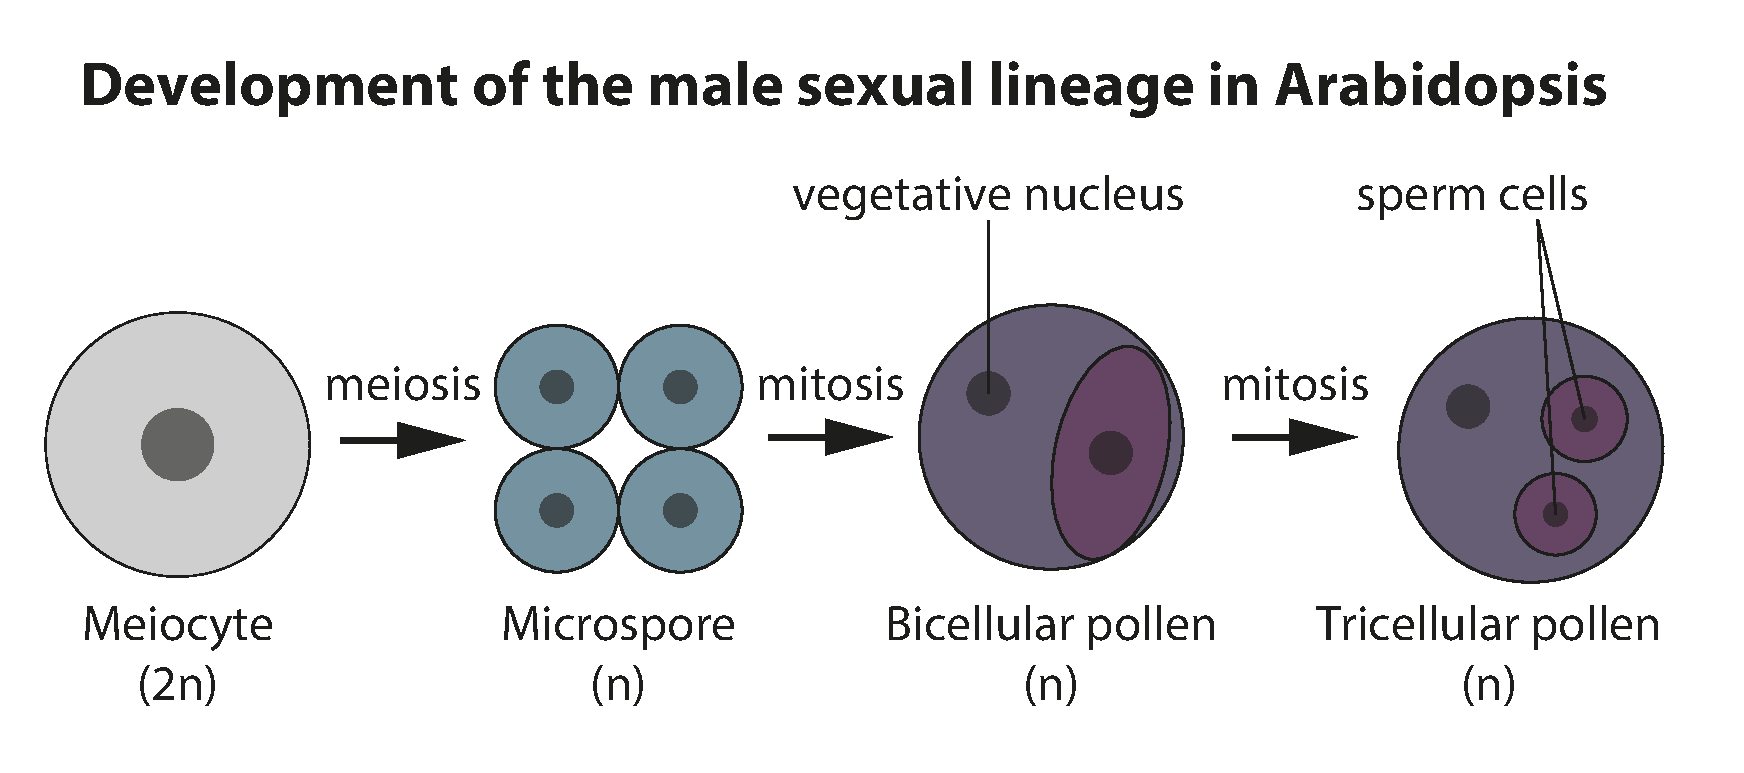
\includegraphics[width=1\textwidth]{Chapter1/Figs/male_sex_dev.pdf}
\caption{An overview of the development of the male sexual lineage in \textit{Arabidopsis}. Figure adapted from \cite{RN199}}
\label{fig:male_sex_dev}
\captionsetup{font=small}
    \caption*{\cite{RN199}}
\end{figure}

AGO proteins play crucial roles in sRNA pathways during reproduction. Recent findings have shown that during male meiosis, AGO1, AGO2, and AGO5 — proteins involved in post-transcriptional gene silencing (PTGS) — are localised in either the nucleus or cytoplasm, whereas AGO4 and AGO9 — associated with transcriptional gene silencing (TGS) — are found exclusively in the nucleus. \cite{RN149}. This study also provided an overview of the expression and localisation of several AGOs throughout meiosis, underscoring their dynamic expression and critical roles in germline development. Additionally, the presence of AGO1 and AGO5-bound micro RNAs (miRNAs) in meiocytes suggests that the miRNA pathway may be involved during meiosis \cite{RN149}. Furthermore, AGO5 and AGO9 have recently been shown to mark reproductive cells, similar to the early segregation of germline cells in animals \cite{RN291}. 

The RdDM pathway and sRNAs play crucial roles not only in germline development in \textit{Arabidopsis}, but also in other plant species. In maize, 21- and 24-nucleotide phased small interfering RNAs (phasiRNAs) are produced in the anthers and are essential for proper anther development \cite{RN292,RN293}. In sorghum, miRNAs were found to be differentially expressed before and after meiosis \cite{RN150}. In \textit{Arabidopsis}, cucumber, and soybean, several miRNAs are conserved and preferentially expressed in meiocytes, though their overall abundance is lower compared to somatic tissues \cite{RN151}. In rice, the ARGONAUTE protein OsAGO18 is specifically expressed in meiocytes, where it facilitates the accumulation of miRNA-triggered secondary siRNAs and regulates genes involved in pollen grain development \cite{RN153}. Additionally, the maintenance of CHH methylation through the RdDM pathway—particularly via RDR2, a critical component of RdDM—is necessary for both male and female sexual development in rice \cite{RN154}. Moreover, rice sporogenesis depends on the degradation of the germline-specific ARGONAUTE protein MEL1, which prevents off-target effects from rogue phasiRNAs; disruption of this process results in a semi-sterile phenotype \cite{RN155}.

Recent work identified male sexual lineage specific DNA methylation reprogramming in the \textit{Arabidopsis} germline, which will be discussed in detail in Chapter 2. Briefly, male meiocytes maintain high levels of CG and CHG methylation when compared to somatic canonical RdDM (cRdDM) loci levels, and a relatively low level of CHH methylation. However, in the CHH context, there is distinct hypermethylation at selected, sexual lineage specific loci (HyperTEs), including novel targets of RdDM activity. Additionally, \textit{de novo} gene-associated methylated loci (MetGenes) were also identified, including a meiosis-specific gene that was mis-spliced when methylation was disrupted \cite{RN199}. Recent evidence suggests that the biogenesis of these 24-nt sRNAs occurs in the somatic nurse cell layer surrounding the meiocytes, known as the tapetum \cite{RN187}. 

Similarly, in the female germline, the surrounding somatic tissue synthesises RNA polymerase IV-dependent 24-nt sRNAs from siren (siRNA in the endosperm) loci \cite{RN164,RN163,RN162}. Like the tapetal nurse cell-derived sRNAs that catalyse DNA methylation in male meiocytes, these siren loci-derived sRNAs are also dependent on CLSY3 and CLSY4 \cite{RN162}. However, there is little overlap between the loci targeted by these two sets of sRNAs, and even less between siren loci across different species \cite{RN163}. Despite their distinct origins, siren loci-derived sRNAs in \textit{Brassica rapa} similarly catalyse DNA methylation, predominantly at protein-coding genes, thereby regulating gene expression in the ovule \cite{RN165}. Furthermore, it has been recently shown that 24nt sRNAs accumulate in rice zygotes, which overlap gene rich, distinct loci from paternally derived sRNA loci \cite{RN166}, highlighting the conserved nature of 24 nucleotide sRNA driven DNA methylation reprogramming in both the male and female sexual lineage. The importance of RdDM in embryonic development is further underpinned by a recent study that showed embryos resulting from a maternal RdDM mutant cross result in incorrect gene expression in the endosperm and a reduction in seed viability \cite{RN167}.

\subsection{Illumina library preparation and sequencing by synthesis}

Over the past two decades, next-generation sequencing (NGS) technologies have transformed biological sequencing by dramatically improving speed, accuracy, and data output. These advancements enable both high-throughput and low-input sequencing while maintaining exceptional fidelity.

Illumina sequencing technology requires constructing a sequencing library tailored to the specific sample, by either converting genomic DNA (gDNA) or complementary DNA (cDNA) into a fragmented library for sequencing. Various workflows are available to accommodate different throughput requirements and starting materials. These include on-bead tagmentation \cite{RN314}, which reduces preparation time, AmpliSeq amplicon library preparation \cite{RN315}, and the widely used adapter ligation workflow \cite{RN316}.

The construction of an Illumina sequencing library using adapter ligation typically involves several key steps (an overview is presented in Figure \ref{fig:illumina_library_prep} \cite{RN312}). For DNA sequencing, the process begins with DNA extraction. In the case of plant material, this may involve a CTAB extraction \cite{RN321} using chloroform to obtain ultra-pure DNA, free of secondary metabolites and proteins, though various other DNA extraction methods and kits can also be used. For RNA sequencing, an additional step is required after extraction, namely reverse transcription to convert RNA into complementary DNA (cDNA) \cite{RN312,RN317}.

\begin{figure}[htbp!] 
\centering    
    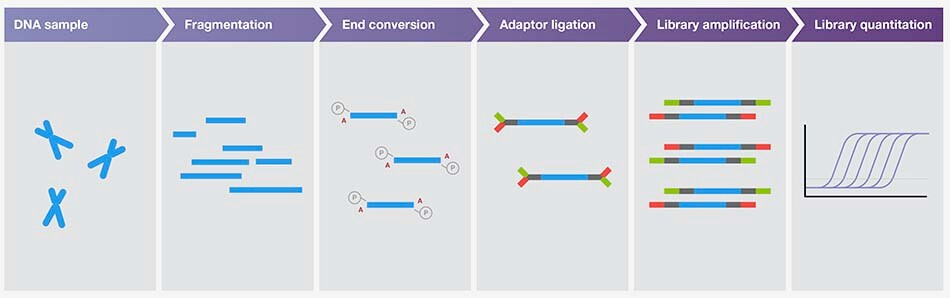
\includegraphics[width=1\textwidth]{Chapter1/Figs/illumina_library_prep.jpg}
\caption{An overview of the steps involved in library preparation for Illumina sequencing \cite{RN312}}
\label{fig:illumina_library_prep}
\captionsetup{font=small}
\end{figure}

Once extracted, gDNA must be fragmented, as Illumina sequencing is optimised for relatively short sequences, typically in the 300–600 bp range. This fragmentation can be achieved through either mechanical shearing or enzymatic digestion. Mechanical shearing, often performed using high-frequency acoustic sonication, breaks the DNA’s phosphodiester backbone. The optimal force and duration of sonication vary depending on the instrument and experimental needs and should ideally be determined experimentally \cite{RN312}.

Following an end repair step, where the sheared DNA fragments are repaired (polymerase activity) or blunted (exonuclease activity) and the ends phosphorylated, adapters are ligated to the ends of the fragments. Adapters are a pair of oligonucleotides which facilitate the clonal amplification step used during Illumina sequencing. The adapters are normally made up of 3 sections. Firstly, a complementary end which forms the adapter duplex, this is annealed to the ends of the insert. Secondly, the adapters contain unique index sequences which can be used to demultiplex several samples that were sequenced together on the same flow cell. Finally, the adapter sequences contain a non-complementary P5 and P7 end (so-called due to their binding site to the flow cell), which prevents self-ligation \cite{RN312,RN317}. 

After the adapter ligation step, PCR amplification may follow, which allows for a lower sample input, however it can introduce GC bias, polymerase errors, chimeric sequences or amplification bias, which might hinder SNP discovery and \textit{de novo} genome assembly. Therefore, given an amount of starting material, the lowest possible cycles of PCR must be performed to prevent these effects \cite{RN312,RN317}.

After fragmentation, adapter ligation and PCR amplification, a size- selection and clean-up step is usually performed, to ensure uniform library fragment size and remove excess unligated adapters or adapter dimers. The clean-up step may be performed using agarose or sometimes polyacrylamide gels, or more commonly using magnetic beads which can bind and elute DNA in a size-specific manner depending on the bead to sample DNA ratio. These steps help to increase data output, reduce noise and ensure the quality of the data output (as Illumina sequencing has an optimal insert length at which the sequencing is most accurate) \cite{RN312,RN317}.

\begin{figure}[htbp!] 
\centering    
    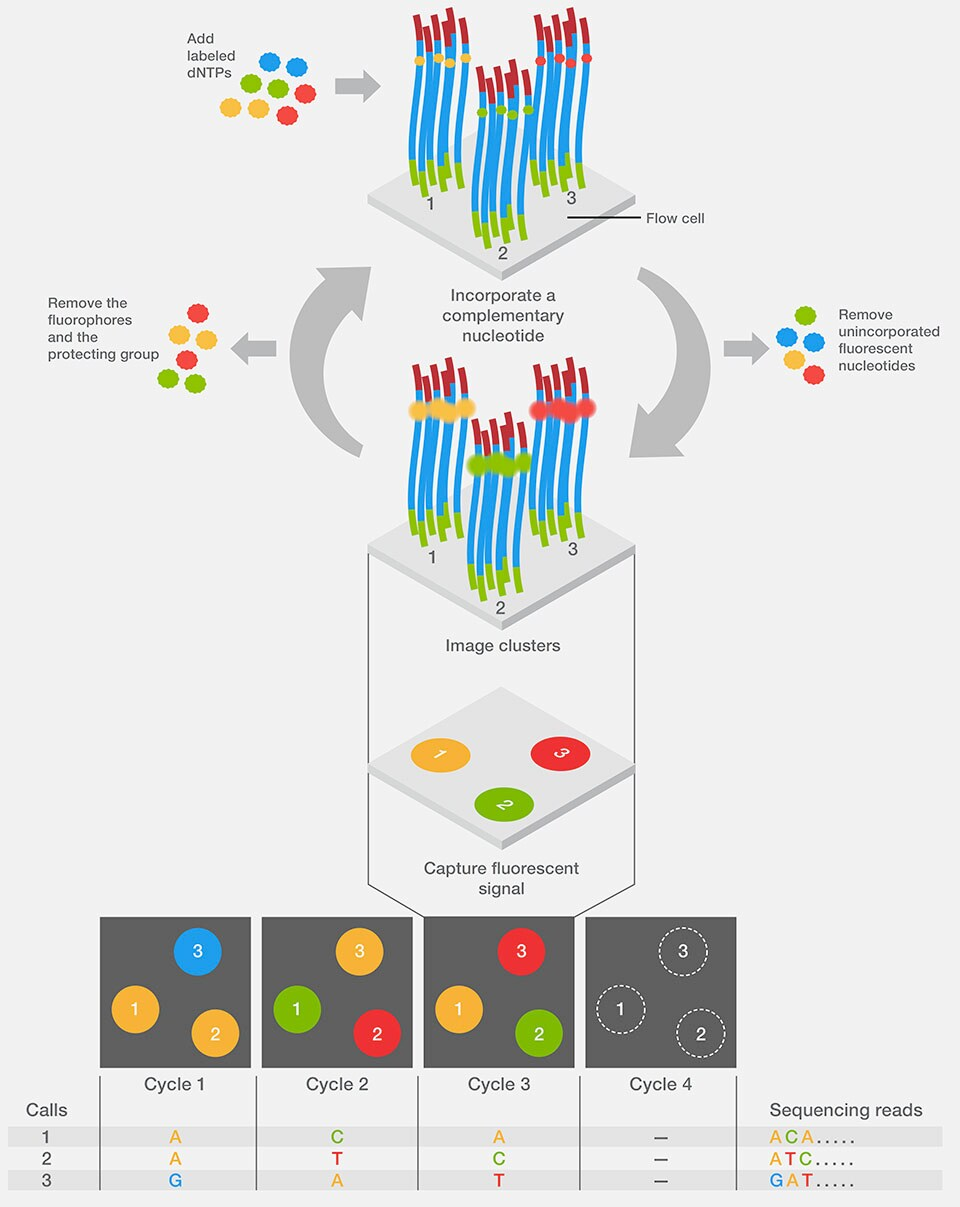
\includegraphics[width=1\textwidth]{Chapter1/Figs/illumina-sequencing.jpg}
\caption{An overview of sequencing by synthesis \cite{RN313}}
\label{fig:illumina_sequencing}
\captionsetup{font=small}
\end{figure}

Following an accurate library quantification step, the Illumina libraries are ready to be sequenced. Briefly, the adapter ligated DNA fragments are flushed across the flow cell where they hybridise to immobilised complementary primer sequences on the flow cell. The fragments are clonally amplified using bridge amplification to form clusters of identical reads across the flow cell. The forward reads are sequenced by priming and extending the first read using fluorescently tagged dNTPs, which compete to be incorporated into the growing chain. After each cycle of the incorporation of the fluorescently tagged base, the clusters are excited by a light source and the fluorescent signal is recorded (an overview of how bases are sequenced is shown in Figure \ref{fig:illumina_sequencing} \cite{RN313}). In paired-end sequencing, following the sequencing of the forward read, the read product is washed away, the fragments are extended once again and the original forward read is cleaved off, followed by sequencing of the reverse read in a similar manner as before \cite{RN313}. 

\subsection{Detecting methylated cytosines in NGS sequencing}

To characterise the methylation profile of a sample, various treatment protocols can be applied prior to Illumina library preparation to facilitate sequencing-based methylation analysis. These use specific chemistries or enzymatic activities to selectively alter or protect methylated bases.

\begin{figure}[htbp!] 
\centering    
    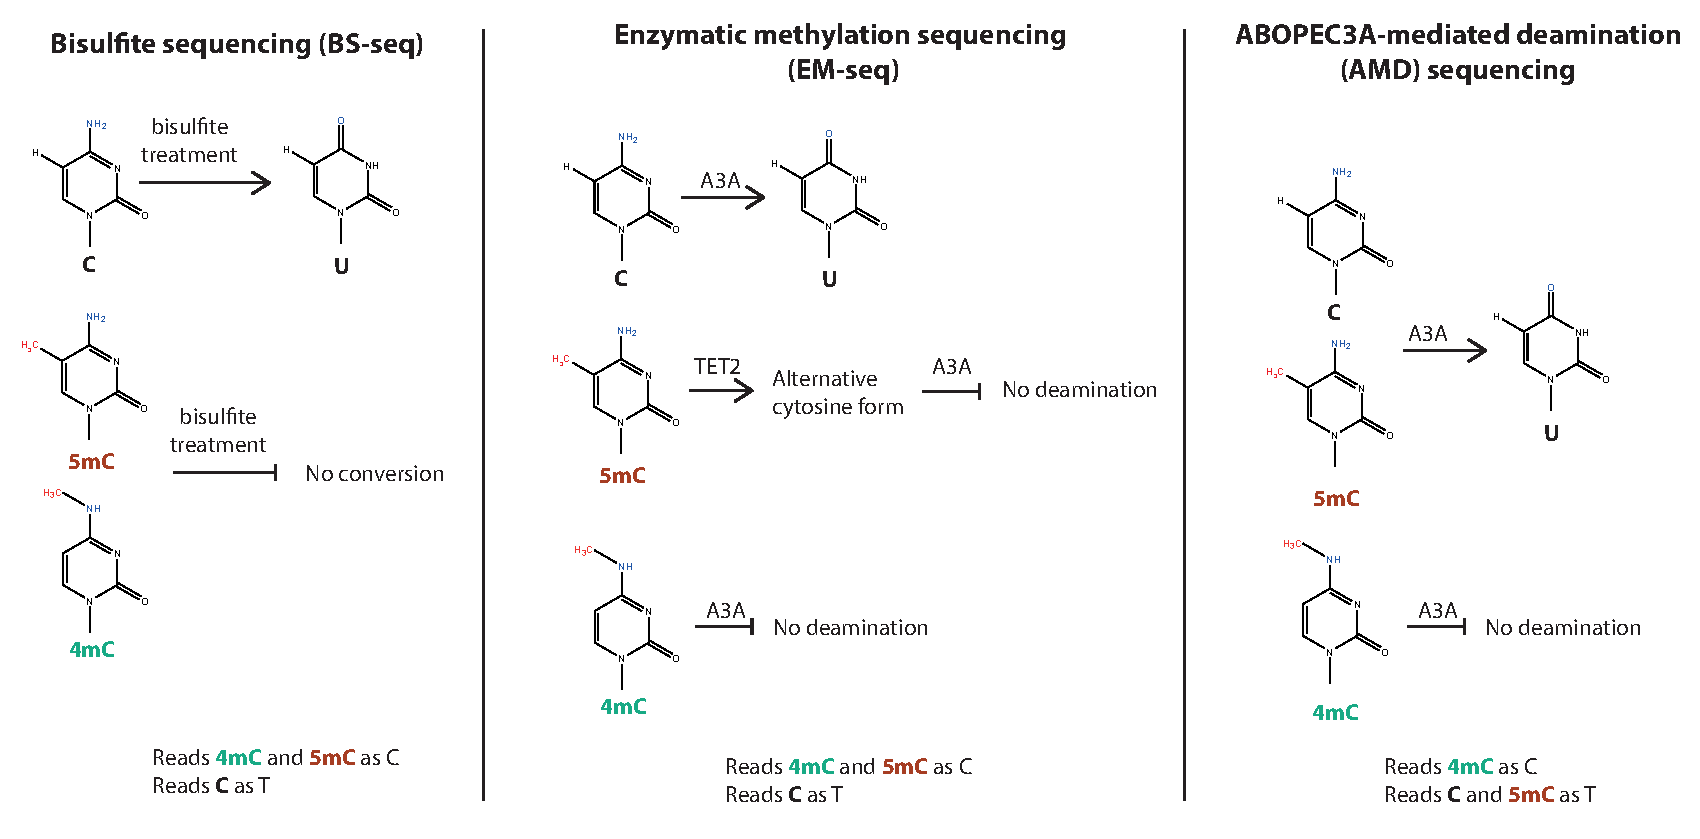
\includegraphics[width=1\textwidth]{Chapter1/Figs/sequencing_chemistries.pdf}
\caption{An overview of the chemistries of modified base sequencing: BS-seq, EM-seq and AMD-seq.}
\label{fig:sequencing_chemistries}
\captionsetup{font=small}
\end{figure}

The most widespread sequencing method utilised to sequence methylated DNA is bisulfite sequencing. The DNA fragments are treated with sodium bisulfite, which (through a series of intermediate steps) selectively deaminates unmethylated cytosines, resulting in uracil. At the same time, due to the structural changes introduced by the methyl group in 5-methylcytosine and N4-methylcytosine, these modified bases are protected from deamination (first panel, Figure \ref{fig:sequencing_chemistries}). Consequently during sequencing, the unmethylated cytosines that were converted to uracils are read as thymines. In contrast, the methylated bases remain as cytosines, thereby enabling their identification by aligning bisulfite sequencing data to reference genomes using specialised bioinformatics tools, such as Bismark \cite{RN229}. Bisulfite sequencing methods are robust and have also been developed for single-cell or very low input sequencing \cite{RN207}. The downsides of bisulfite sequencing are that they do not distinguish between the methylated bases (4mC or 5mC) \cite{RN200} and that bisulfite sequencing itself can introduce DNA damage due to the protocol requiring extremes of pH and temperature, resulting in depyrimidination of DNA \cite{RN318}.

Alternative enzymatic methods have been developed to combat some of the challenges of bisulfite sequencing, namely APOBEC3A-mediated deamination sequencing (AMD-seq) \cite{RN188}, which allows for reading 4mC as Cs specifically, as well as enzymatic methylation sequencing \cite{RN319} (EM-seq) which is a direct alternative to bisulfite sequencing, reading both 5mC and 4mC as Cs during sequencing, but without significant DNA damage.

Both EM-seq and AMD-seq rely on the ability of APOBEC3A, which is an enzyme originally described in primates \cite{RN320}, to deaminate a variety of cytosine forms to uracil. Namely, APOBEC3A can deaminate both unmodified cytosines and 5mC. However, 4mC is protected from deamination by APOBEC3A, so following enzymatic treatment, an Illumina sequencing library is constructed and all unmethylated cytosines as well as 5mC will be read as Ts during sequencing, and only 4mC will be read as Cs \cite{RN188} (Figure \ref{fig:sequencing_chemistries} third panel). EM-seq introduces an additional step, whereby prior to ABOBEC3A treatment, the Tet methylcytosine dioxygenase 2 (TET2) enzyme specifically converts 5mC sites to alternative cytosine forms which are not substrates of APOBEC3A. As a result, similar to traditional bisulfite sequencing, in EM-seq, both 5mC and 4mC are be read as Cs while unmethylated cytosines are be read as Ts (Figure \ref{fig:sequencing_chemistries} second panel).

\section{Thesis outline}

This thesis explores the dynamics of RdDM and DNA methylation after meiosis in the male sexual lineage of \textit{Arabidopsis} and in the embryo of \textit{Marchantia}.

In Chapter 2, the expression of CLSY chromatin remodellers, Pol IV, and Pol V in post-meiotic anthers of \textit{Arabidopsis} is investigated. This is followed by the sequencing and comparison of sRNA profiles from microspores, sperm cells, and sperm nuclei with other published germline and somatic datasets. Potential reactivation of sRNA biogenesis at cRdDM loci is revealed, and non-canonical RdDM pathways are implicated in sRNA biogenesis post-meiosis. Additionally, sRNA clusters derived from MetGenes and ATGP2N TEs in sperm cells are identified, along with a cluster of sperm-specific heterochromatic loci.

In Chapter 3, the sRNA and DNA methylation profiles of \textit{Marchantia} embryos are examined. MetGenes are defined in the sporophyte, and their connections to TE loci are identified. A method for isolating, imaging, and sequencing early embryos is tested, developed, and presented. Nuclear reporter lines are constructed to observe the phenotypic effects of knocking out paternal 4mC methylation in the embryo.

Each chapter contains a detailed materials and methods section, as well as appendices with supplemental information. In Chapter 4, the results are summarised in a broader context, and potential future directions, reflections, and limitations of the work are discussed.
%!TEX root = ../thesis.tex
%*******************************************************************************
%****************************** Second Chapter *********************************
%*******************************************************************************

\chapter{The spatiotemporal expression of RdDM components and small RNA landscapes in the germline of \textit{Arabidopsis thaliana}}

\ifpdf
    \graphicspath{{Chapter2/Figs/Raster/}{Chapter2/Figs/PDF/}{Chapter2/Figs/}}
\else
    \graphicspath{{Chapter2/Figs/Vector/}{Chapter2/Figs/}}
\fi

\section{Abstract}

This chapter explores the spatiotemporal expression of RdDM components and the sRNA landscapes in the male germline of \textit{Arabidopsis thaliana}. By employing a combination ofimaging fluorescent reporter lines, small RNA sequencing, and bioinformatics analysis the dynamics of RdDM-associated factors during different stages of pollen development were investigated. It was demonstrated that the expression of key RdDM components such as NRPD1 and NRPE1 is tightly regulated, with NRPD1 showing tapetum-specific expression and NRPE1 being active in both germline and somatic tissues. Furthermore, CLSY3 expression was found to be confined to the tapetum and no other CLSY chromatin remodeler expression was detected after meiosis. Further analysis of the sRNA profiles reveals that the sperm cell harbors a distinct small RNA profile, uncoupled from known CLSY-dependent loci, suggesting a shift towards non-canonical RdDM pathways post-meiosis. 

\section{Introduction}

It was previously thought that DNA methylation largely remained stable across reproductive cells in plants, due to its close association with the regulation of transposon activity \cite{RN247} and therefore genome integrity. Global demethylation does occur in companion cells of the germline, however, via passive or active demethylation. The former is due to decreased expression of MET1, leading to a lack of maintenance of methylation during DNA replication in the central cell. The latter is due to active demethylation by DEMETER (DME), which demethylates CG sites in the vegetative nucleus \cite{RN235,RN57}. This leads to the synthesis of 21nt epigenetically active small interfering RNAs (easiRNAs) in the vegetative cell from typically silenced TEs. As the vegetative cell is a terminal tissue rather than part of the germline, the destabilising effects to the genome is not of evolutionary concern. The easiRNAs produced from the vegetative cells move into the sperm cells where they accumulate and silence complementary target DNA sites through RdDM \cite{RN14,RN16}.

The RdDM pathway provides some of the essential communication between different cell types in reproductive tissue. AGO6 and AGO9 are a close paralog of AGO4 expressed in reproductive cells, which binds to 24nt RNA to direct RdDM. AGO6 is expressed in the shoot apical meristem, and there is increasing evidence that 21-22 nt secondary siRNAs (deriving from the miRNA pathway) can associate with AGO6 and participate in RdDM \cite{RN133,RN61,RN33}. Arabidopsis ago9 produces multiple megaspore mother cells (MMCs) in the female germline. Here, AGO9 is in the surrounding somatic nucellar cells, suggesting that sRNAs and corresponding essential RdDM machinery are transferred between cells.  TEs that are constitutively silenced in wildtype plants were reactivated in ago9 embryo sacs, suggesting a pathway similar to the mammalian piRNA pathway previously discussed \cite{RN14}.

Recent work identified male sexual lineage specific DNA methylation reprogramming in the \textit{Arabidopsis} germline. In general, male meiocytes maintain high levels of CG and CHG methylation when compared to somatic canonical RdDM loci levels, and a relatively low level of CHH methylation. However, in the CHH context, there is distinct hypermethylation at selected, sexual lineage specific loci (HyperTEs), including novel targets of RdDM activity. Further, de novo gene associated methylated loci were also identified (MetGenes), including a meiosis specific gene (Figure \ref{fig:SLH_SLM}) \cite{RN199}.

\begin{figure}[htbp!] 
\centering    
    \includegraphics[width=0.7\textwidth]{Chapter2/Figs/Intro/SLH_SLM_methylation.pdf}
\caption{}
\label{fig:SLH_SLM}
\captionsetup{font=small}
    \caption*{}
\end{figure}

Further, it was discovered that meiocytes themselves are quiescent in sRNA biogenesis. The biogenesis of these germline specific siRNAs is in the somatic tapetal tissue and is associated with the chromatin remodeller CLASSY3. Nurse cell-derived siRNAs are then transported into the meiocyte from the tapetum, inducing DNA methylation at HyperTE loci. MetGene loci can be uniquely targeted for methylation in the meiocyte by imperfectly matching siRNA derived from HyperTEs. These nurse-cell derived siRNAs inform the entire male sexual lineage specific methylation reprogramming, from meiocyte to sperm (Figure \ref{fig:Jincheng_abstract}) \cite{RN187}.

\begin{figure}[htbp!] 
\centering    
        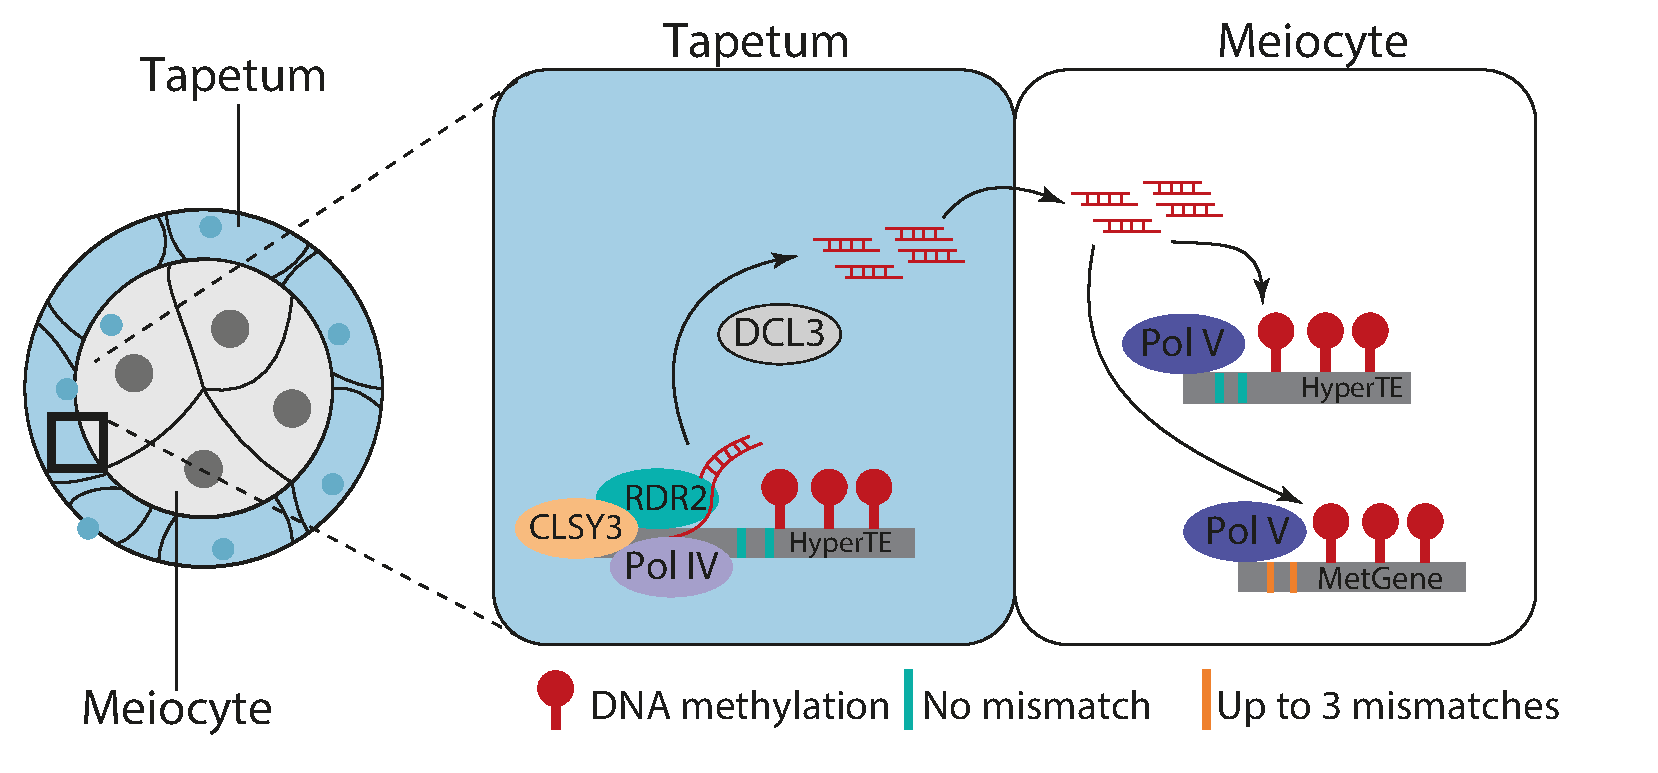
\includegraphics[width=0.7\textwidth]{Chapter2/Figs/Intro/Jincheng_paper_abstract.pdf}
\caption{}
\label{fig:Jincheng_abstract}
\captionsetup{font=small}
    \caption*{}
\end{figure}
\clearpage

The mechanism of movement of sRNA between companion and germline cells needs more evidence, however there is extensive evidence of cross-cellular RNA movement. Plasmodesmata provide a cytoplasmic network between cells (such as the tapetum and meiocyte) which allows nutrient transport but have also been shown to allow RNA movement between cells \cite{RN130,RN132,RN128}.

The aim of this chapter is to shed light on how this germline-specific sRNA and DNA methylation profile changes after meiosis. Namely, to investigate the sRNA profiles of the microspore and sperm cells, and to examine the expression of RdDM associated key factors involved during the development of male-sexual lineage.  

\section{NRPD1 is expressed in the tapetum, microspores but not in meiocytes}

Since RNA polymerase IV and V preferentially associate with methylated RNA, RdDM is thought of as a self-reinforcing pathway. Therefore the observation that there are few perfect matching 24nt sRNAs in MetGenes in Arabisopsis meiocytes, it was hypothesised that the Pol IV dependent pathway is quiescent and that the sRNAs directing DNA methyaltion at MetGenes are produced from HyperTE loci in the tapetum that target HyperTE and MetGene methylation in the meiocyte \cite{RN199,RN187}. To confirm this expression pattern, pNRPD1::NRPD1-eGFP and pNRPE1::NRPE1-eGFP fluorescent reporter lines (of the largest subunits of RNA Polymerase IV and V respectively\cite{RN33}) were constructed by Dr. Jincheng Long.

The columella in the root tip of Arabidopsis is hypermetylated in the CHH context \cite{RN261}, the root tip was imaged to screen and select the best lines selected for further imaging (Figure\ref{fig:Pol4_5_roots}).

\begin{figure}[htbp!] 
\centering    
    \includegraphics[width=1\textwidth]{Chapter2/Figs/Figure3_Pol4_anther_gynecium.pdf}
\caption{\textbf{NRPD1 is expressed in the tapetum, microspore and gynoecium.}}
\label{fig:Pol4_anther}
\captionsetup{font=small}
    \caption*{NRPD1 expression in meiocyte stage anthers in the tapetum and surrounding somatic cells(first row, third column (GFP, green, white arrows), and expression in microspores (second row third column, white arrows). NRPD1 is also expressed in both the germ and somatic cells of the meiocyte stage gynoecium (third row (GFP, green)). Scale bar 10 $\mu$m.}
\end{figure}

Meiocytes are surrounded by the tapetum - a somatic tissue layer of nurse cells with cytoplasmic connections to meiocytes through plasmodesmata. As expected, NRDP1 expression was confined to the tapetal layer and surrounding somatic anther tissue in meiocyte stage anthers (Figure \ref{fig:Pol4_anther}). Once meiocytes undergo meiosis, the plasmodesmatal connection to the tapetum ceases and the meiocytes are surrounded by callose cell walls. At the microspore stage, the germline cells express NRPD1 (Figure \ref{fig:Pol4_anther} second row, \ref{fig:Pol4_germ} first and second rows). NRPD1 was also expected to be expressed strongly in the maternal reproductive tissue \cite{RN165} which was confirmed in several independent reporter lines (Figure \ref{fig:Pol4_anther}, row three).

Following a further two cell divisions, the bicellular and tricellular pollen grains are produced, neither of which express NRPD1 (Figure \ref{fig:Pol4_germ}, rows 3 and 4). However, it must be added that the expression levels of the best NRPD1 reporter lines were a lot lower and more diffuse than the expression of NRPE1 or CLSY3 reporter lines (Figures \ref{fig:CLSY3_anther}, \ref{fig:Pol4_5_roots}). Further, expression in germline tissues wasn't consistent even in lines that exhibited strong root signal (Figure \ref{fig:Pol4_germ}, Figure \ref{fig:Pol4_germ_no_expression}). As these results are from screening 37 independent transformants from the same transformation event, it would be worth constructing new transformants perhaps with a stronger fluorescent reporter (such as tdTomato) to corroborate these results, and confidently confirm whether NRPD1 is expressed in the pollen. 


\begin{figure}[htbp!] 
\centering    
    \includegraphics[width=0.8\textwidth]{Chapter2/Figs/Figure4_Pol4_germline.pdf}
\caption{\textbf{NRPD1 is expressed in microspores, but its expression is absent in pollen}}
\label{fig:Pol4_germ}
\captionsetup{font=small}
    \caption*{NRPD1 expression early and late microsproes (first and second rows, third column (GFP, green, white arrows), and expression in microspores (second row third column, white arrows). NRPD1 however us not expressed in bicellular or tricellular pollen (third and fourth rows (DAPI, blue GFP, green). Scale bar 10 $\mu$m.}
\end{figure}

\section{NRPE1 is expressed in both somatic and germline tissues in \textit{Arabidopsis} anthers}

According to methylation and 24nt sRNA datasets,  PolV-dependent pathway of RdDM be active in the somatic tapetal layer and meiocytes, but it wasn't clear what happens after meiosis in microspores and pollen. As before, strong nuclear signal was confirmed in the root tip (Figure \ref{fig:Pol4_5_roots}).  NRPE1 is strongly expressed in meiocytes, tapetum and in the surrounding somatic tissues of the meiocyte stage anther (Figure \ref{fig:Pol5_germ}, first row). This expression also persists into both soma and germline of microspore stage anthers and the female meiocyte stage gynoecium (Figure \ref{fig:Pol5_germ} second and third rows respectively), indicating that the RNA polymerase V pathway of RdDM is active in both somatic and germline cells of the anther. As we know RdDM is highly active in maternal reproductive tissue, the expression of NRPE1 was confirmed in this tissue as well (Figure \ref{fig:Pol5_germ}, third row).

\begin{figure}[htbp!] 
\centering    
    \includegraphics[width=1\textwidth]{Chapter2/Figs/Figure5_Pol5_germline.pdf}
\caption{\textbf{NRPE1 is expressed in the tapetum, meiocyte, microspores and gynoecium}}
\label{fig:Pol5_germ}
\captionsetup{font=small}
    \caption*{NRPE1 expression in meiocyte stage anthers in the tapetum, meiocyte and surrounding somatic cells(first row, third column (GFP, green, white arrows), and expression in microspores (second row third column, white arrows). NRPE1 is also expressed in both the germ and somatic cells of the meiocyte stage gynoecium (third row (GFP, green)). Scale bar 10 $\mu$m.}
\end{figure}


\section{CLSY3 is expressed in the tapetum of meiocyte stage anthers and in the gynoecium}

CLSY3 chromatin remodeller drives sRNA production in the tapetum \cite{RN187} by recruiting Pol IV to discrete loci (including HyperTEs)\cite{RN23}. In accordance with this, the expression on CLSY3 in meiocyte stage anthers is largely restricted to the tapetum (Figure \ref{fig:CLSY3_anther} first row), with diminished expression in the tapetum after meiosis (Figure \ref{fig:CLSY3_anther} second row). CLSY3 is also required for expression of abundant 24nt sRNA in the ovules and therefore it is strongly expressed in the gynoecium and surrounding somatic tissues (Figure \ref{fig:CLSY3_anther}, third row).

\begin{figure}[htbp!] 
\centering    
    \includegraphics[width=1\textwidth]{Chapter2/Figs/Figure1_CLSY3_anther_gynecium.pdf}
\caption{\textbf{CLSY3 is expressed in the tapetum of meiocyte stage anthers and in the gynoecium}}
\label{fig:CLSY3_anther}
\captionsetup{font=small}
    \caption*{CLSY3 is strongly expressed in the nucleus of meiocyte stage tapetal cells (first row (Venus, yellow)), which then diminishes in the senescing tapetum after meiosis in the microspore stage(second row, Venus (yellow)). CLSY3 is also expressed in both the germ and somatic cells of the meiocyte stage gynoecium (third row (Venus, yellow)). Scale bar 10 $\mu$m.}
\end{figure}

However, following meiosis, CLSY3 is not expressed in microspore, bicellular or tricellular pollen stages (Figure \ref{fig:CLSY3_germ}) highlighting the restricted spatiotemporal expression of CLSY3 to produce 24nt sRNAs at HyperTEs and drive methylation of these loci, as well as MetGene loci in the meiocyte. Although endogenous sRNA production is active in the microspore (Figure \ref{fig:Pol4_germ}), and potentially in pollen, CLSY3 does not seem to play a significant role in shaping the 24nt sRNA profiles after meiosis.

\begin{figure}[htbp!] 
\centering    
    \includegraphics[width=0.8\textwidth]{Chapter2/Figs/Figure2_CLSY3_germline.pdf}
\caption{\textbf{CLSY3 is not expressed in the male germline cells}}
\label{fig:CLSY3_germ}
\captionsetup{font=small}
    \caption*{DAPI stained microspore, bicellular or tricellular pollen (second column (DAPI, blue). CLSY3 signal not detected in any germline cells (third row (Venus, yellow). Scale bar 10 $\mu$m}
\end{figure}


\section{HyperTE sRNAs decline proportionally post-meiosis, despite elevated proportional dominance of 24nt sRNAs in sperm cells}

To dissect the dynamics of the sRNA landscape in the germline, sRNA sequencing libraries were constructed for microspores, sperm cells, and sperm nuclei (2 replicates each). These were then compared to meiocyte and tapetum sRNA libraries \cite{RN187}, as well as to somatic sRNA sequencing libraries from the leaf, root and seedling \cite{RN262,RN263,RN264}. 

All three somatic tissues sampled had a strong 21nt and 24nt peak (Figure \ref{fig:sRNA_sizes}A). However, in the germline, except for microspores, the dominant sRNA length was 24nt, with sperm cells and sperm nuclei exhibiting the highest proportional levels of 24nt sRNA (Figure \ref{fig:sRNA_sizes}B).

\begin{figure}[htbp!] 
\centering    
    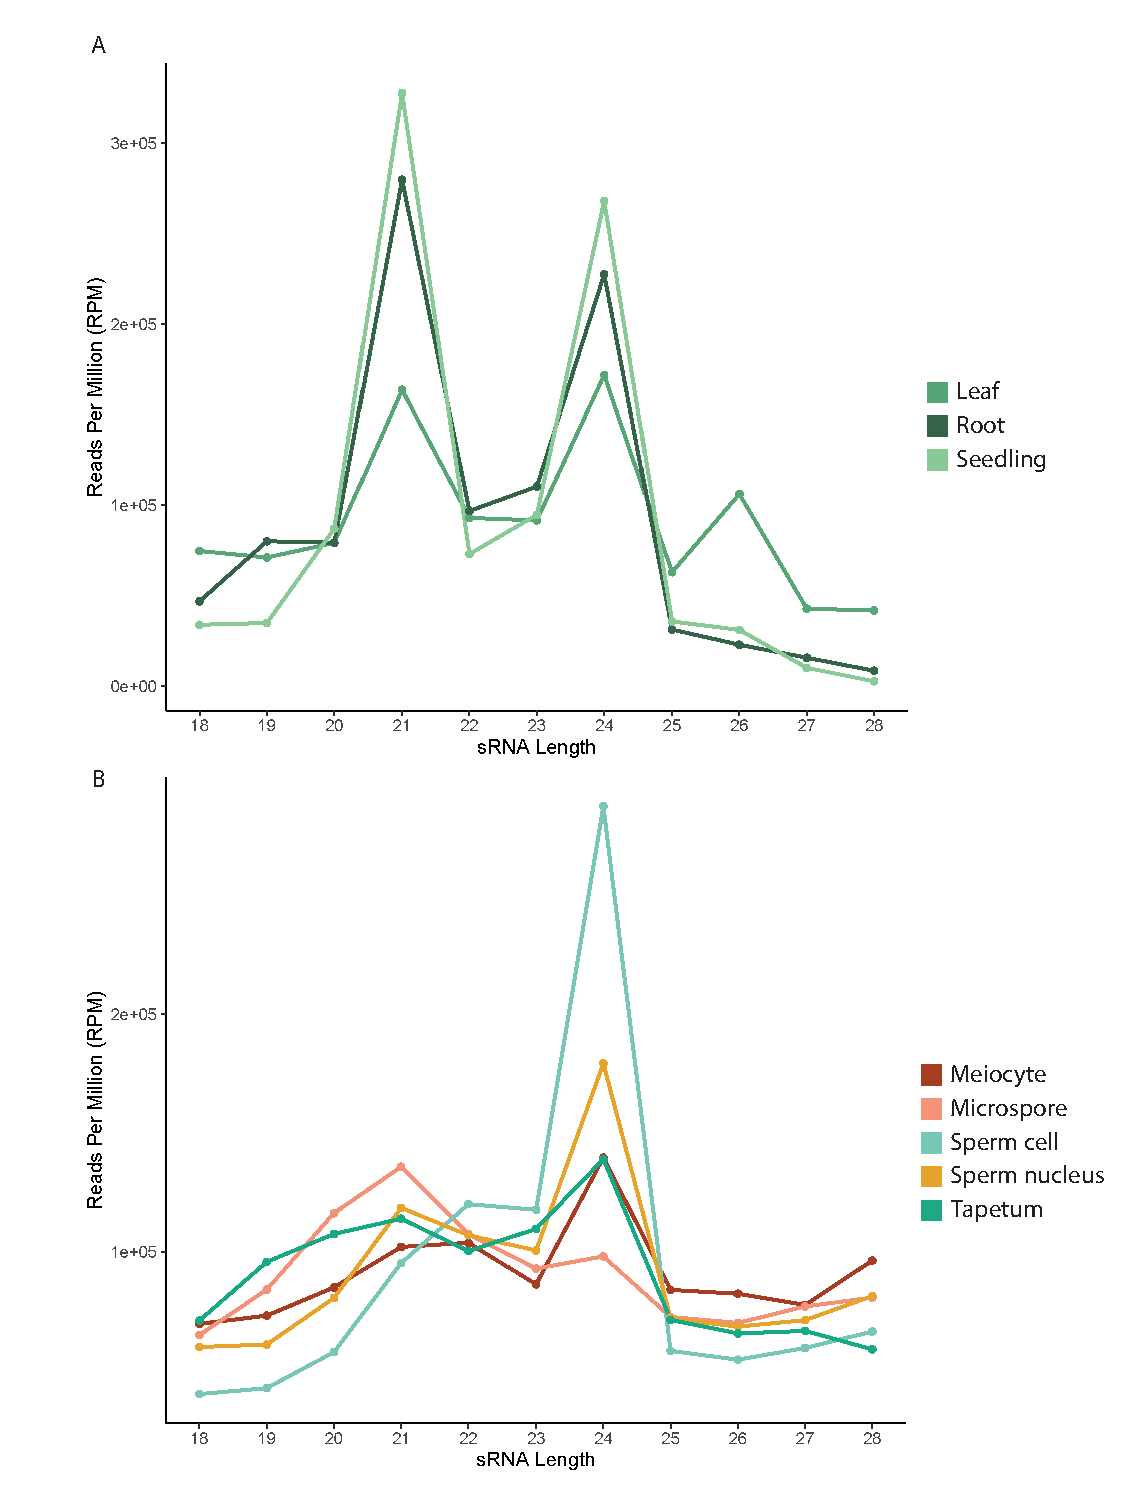
\includegraphics[width=0.8\textwidth]{Chapter2/Figs/Figure6_sRNA_sizes.pdf}
\caption{\textbf{In germline tissues, the dominant sRNA length is 24nt}}
\label{fig:sRNA_sizes}
\captionsetup{font=small}
    \caption*{(A) The size distribution of sRNAs in leaf, root and seedling. X axis: sRNA lengths, Y axis: reads per million (RPM) (B) The size distribution of sRNAs in meiocyte, microspore, sperm cell, sperm nucleus and tapetum. X axis: sRNA lengths, Y axis: reads per million (RPM)}
\end{figure}

When examining genomic features to capture a snapshot of 24nt sRNA distribution in germline tissues, it has been previously shown that HyperTEs dominate the 24nt sRNA landscape in meiocytes \cite{RN187}. However, the proportion of 24nt sRNAs within HyperTE regions gradually declines through cell divisions following meiosis, from meiocytes to sperm cells, suggesting that endogenous HyperTE sRNA production does not continue or ceases in the germline cells after meiosis and the closure of the plasmodesmatal connections to microspores. (Figure \ref{fig:sRNA_pie}A). 

In sperm cells, TE regions become the dominant source of 24nt sRNAs, mirroring the pattern observed in somatic tissues (Figure \ref{fig:sRNA_pie}B). In somatic tissues a large portion of these canonical RdDM loci are known to be associated with CLSY1 and CLSY2 \cite{RN23}. However, in the pollen, neither CLSY1 nor CLSY2 were strongly expressed (Figure \ref{fig:clsy1_2_pollen} suggesting (provided there's endogenous sRNA production in the pollen), these clusters are not strongly associated with the expression of any protein from the CLSY family.

\begin{figure}[htbp!] 
\centering    
    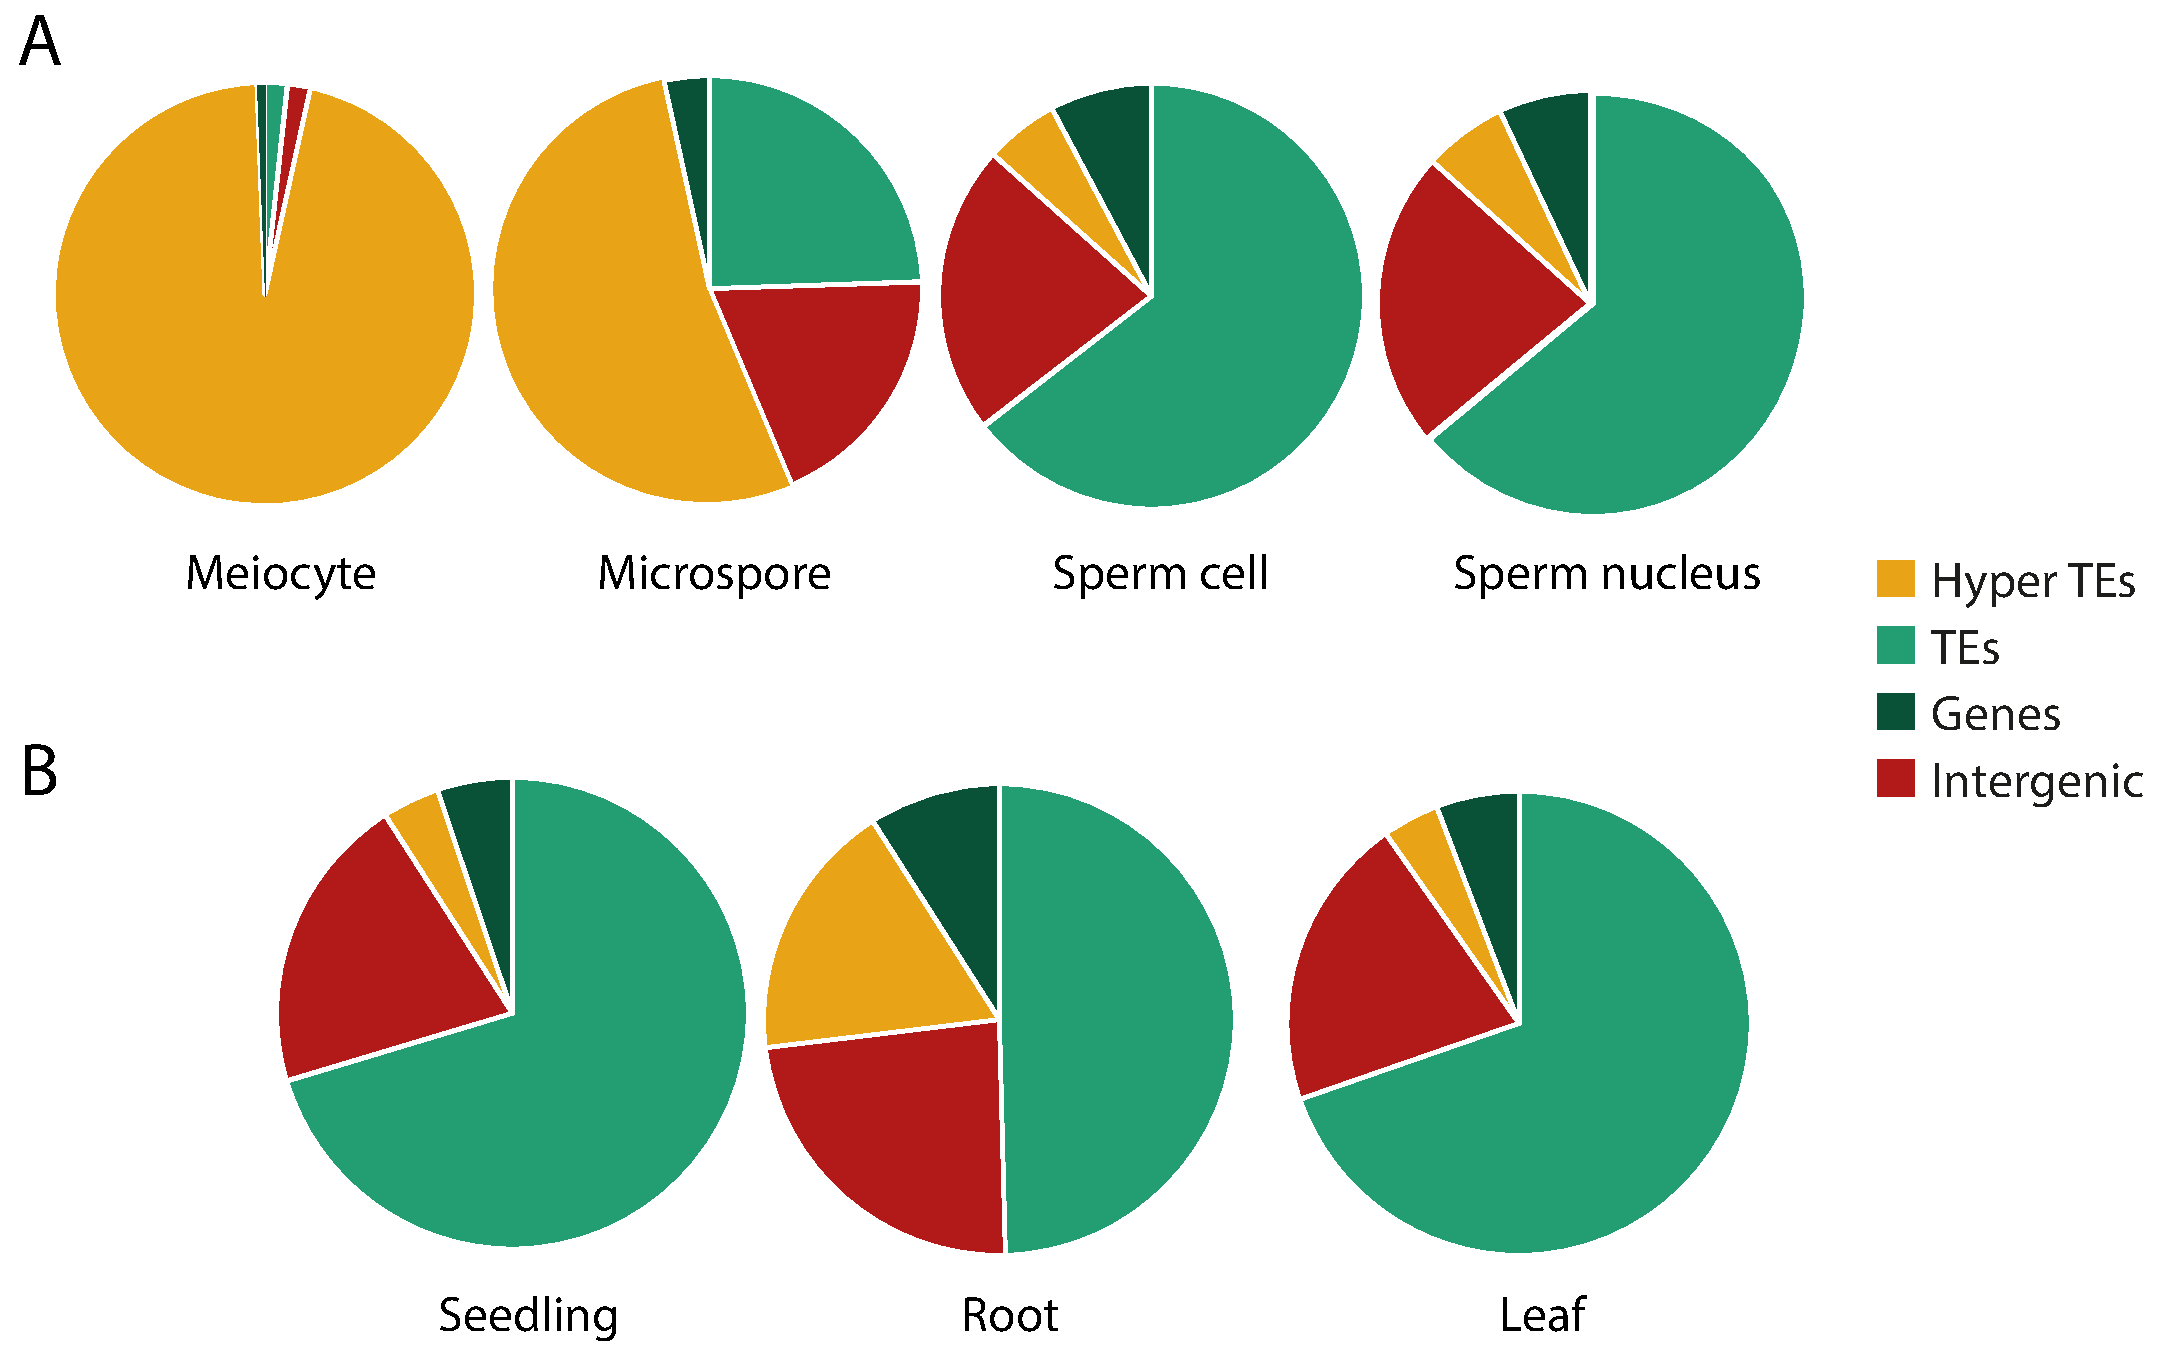
\includegraphics[width=0.8\textwidth]{Chapter2/Figs/Figure7_Pie_charts.pdf}
\caption{\textbf{HyperTE derived 24nt sRNAs decline in proportional abundance after meiosis and throughout pollen development}}
\label{fig:sRNA_pie}
\captionsetup{font=small}
    \caption*{Pie chart showing the proportional mapping of 24nt sRNAs to genomic features of interest: HyperTEs, TEs, Genes, MetGenes and intergenic regions in (A) germline tissue (meiocyte, microspore, sperm cell and sperm nucleus) and (B) somatic tissue (seedling, root and leaf).}
\end{figure}

\section{Sperm Cell sRNA Clusters Are Uncoupled From CLSY-Dependent Loci}

Examining the expression levels of germline-associated CLSY3-dependent loci, HyperTEs, and somatic tissue-associated CLSY1/2-dependent loci, along with canonical RdDM (cRdDM) loci, we can first conclude that, as expected, CLSY1/2-dependent and cRdDM loci exhibit the highest overall abundance of sRNAs in somatic tissues (leaf, seedling, and root). In contrast, most cRdDM loci do not generate sRNAs in the meiocyte, tapetum, or microspore. Interestingly, the sperm cell and sperm nucleus appear to represent an intermediate stage, where sRNA production at cRdDM loci is reactivated though not to the same extent as in somatic tissues (Figures \ref{fig:hm_CLSY3_CLSY1}B,D, \ref{fig:boxplot-MCMS}).

Conversely, in CLSY3-dependent and HyperTE loci, we observe an opposite pattern: 24nt sRNA abundance is highest in the meiocyte, tapetum, and microspore (though somewhat reduced in the microspore at certain loci), while somatic tissues exhibit lower sRNA levels. The sperm cell and sperm nucleus again show intermediate sRNA abundance. Pollen, in particular, displays higher overall levels of 24nt sRNAs from these loci, suggesting they are primarily produced in the vegetative cell. Notably, a subset of HyperTE loci continues to produce sRNAs even in somatic tissues (Figures \ref{fig:hm_CLSY3_CLSY1}A-C, \ref{fig:boxplot-MCMS}).

Since the heatmaps show normalised levels of sRNA against total sRNA levels in each tissue, it must be ensured that these patterns are comparable. To achieve this, 24nt sRNA levels in the cRdDM loci were also normalized against 21nt miRNA levels, as these are assumed to remain constant across cell types. This approach yielded comparable sRNA levels across the tested tissues, validating the observed relative differences in sRNA patterns (Figure \ref{fig:miRNA_norm}).

\begin{figure}[htbp!] 
\centering    
    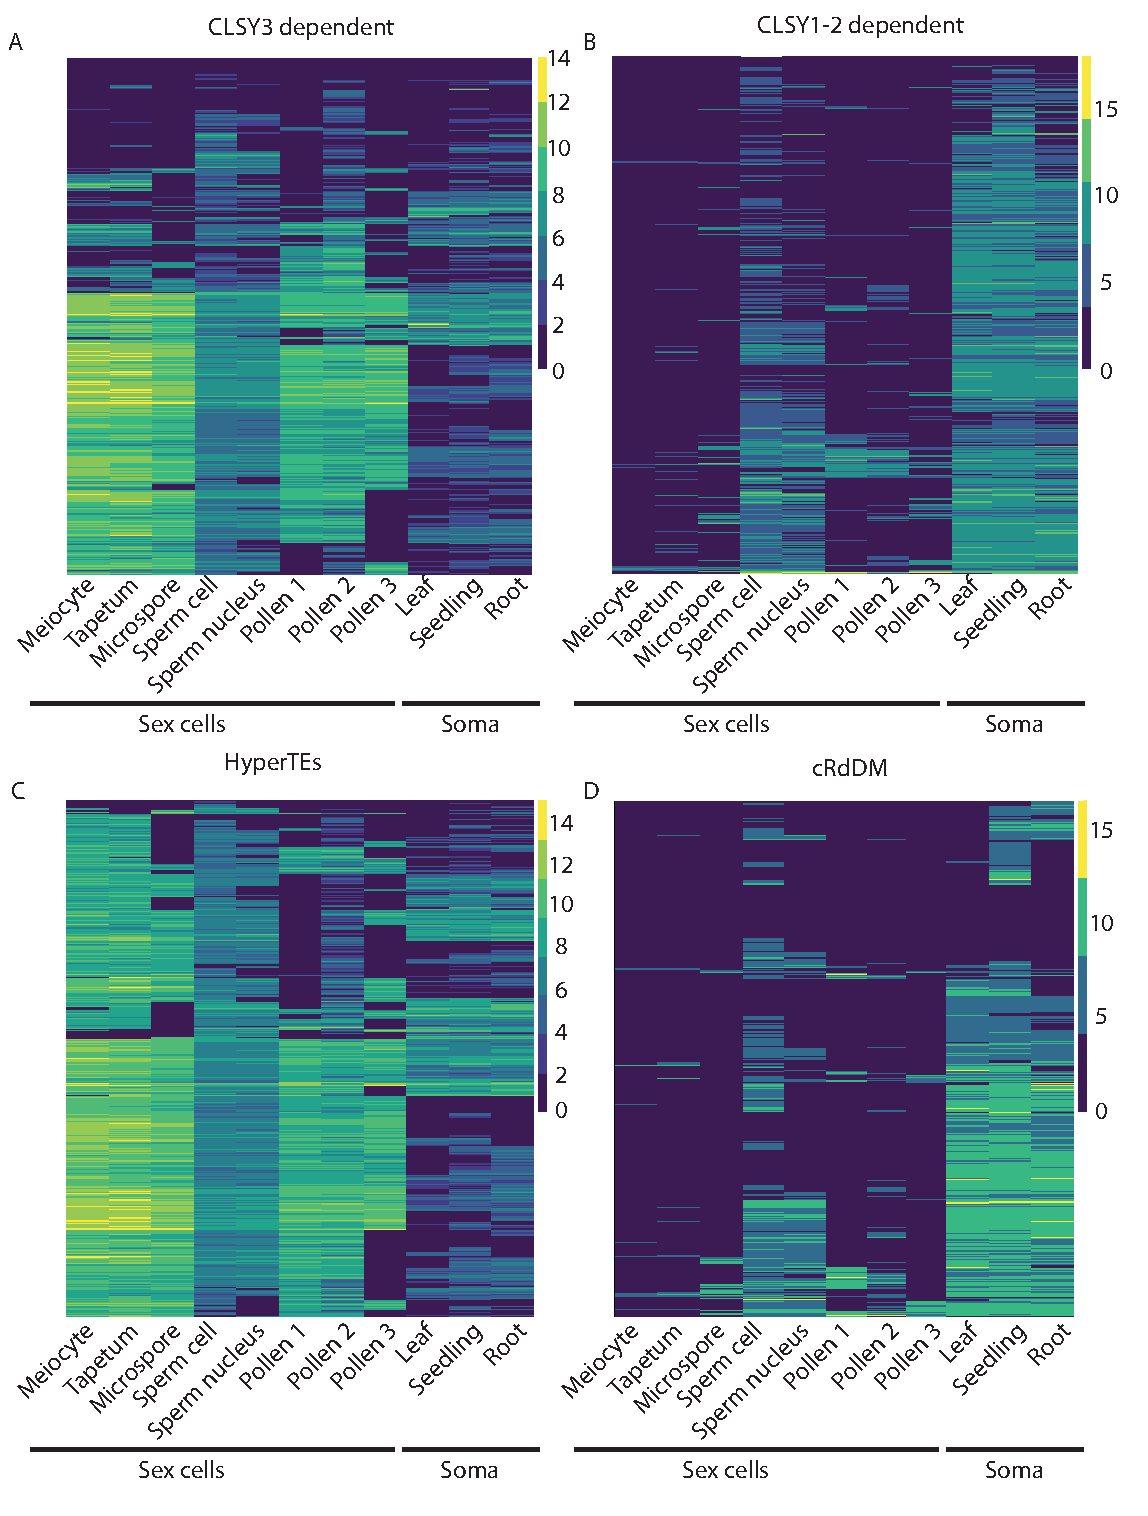
\includegraphics[width=0.8\textwidth]{Chapter2/Figs/Figure8_Heatmaps_CLSY3_CLSY1_2vs_cRdDMs_HyperTEs.pdf}
\caption{\textbf{CLSY3-dependent loci and HyperTEs generate abundant sRNAs in meiocytes and tapetum, as well as in microspores and sperm cells, though to a lesser degree. CLSY1\&2-dependent loci and canonical RdDM loci primarily produce abundant sRNAs in somatic tissues, with intermediate levels in sperm cells.}}
\label{fig:hm_CLSY3_CLSY1}
\captionsetup{font=small}
    \caption*{Heatmaps showing the 24nt sRNA RPKM levels of (A) CLSY3 dependent, (B) CLSY1\&2 dependent, (C) HyperTEs and (D) cRdDM loci in different germline (meiocyte, tapetum, sperm cell, sperm nucleus, pollen) and somatic tissues (leaf, seedling, root). Scale bar shows RPKM values.}
\end{figure}

To further understand the sRNA landscape in sperm and microspore, the sRNA profiles were compared pairwise to somatic tissues as well as other germline tissues, namely the meiocyte. Genome wide, 24nt sRNA abundance in 24nt clusters correlate weakly between the meiocyte and microspore (Figure \ref{fig:MSSVMC_scatters}A), but less so than between tapetum and meiocyte (Figure \ref{fig:scatter_SC_chromatin}A). This correlation is then further reduced between the meiocyte and sperm, indicating that global 24nt sRNA profiles are indeed vastly different between these cell types (Figure \ref{fig:MSSVMC_scatters}B).

Additionally, when comparing sperm cell-specific sRNA clusters between the meiocyte and sperm, and highlighting key genomic features, we clearly see that a significant subset of sperm-specific clusters producing sRNAs overlap with HyperTEs. These clusters have correspondingly high sRNA abundance in the meiocyte, with relatively lower abundance in the sperm cell (Figure \ref{fig:MSSVMC_scatters}B). In contrast, loci with low RPKM values in the meiocyte but high in sperm include a mixture of canonical RdDM loci and other sperm-specific loci that do not overlap with either HyperTEs or cRdDMs.

\begin{figure}[htbp!] 
\centering    
    \includegraphics[width=1\textwidth]{Chapter2/Figs/CLSY_singles_scatterplots.pdf}
\caption{\textbf{}}
\label{fig:clsysingle_scatters}
\captionsetup{font=small}
    \caption*{}
\end{figure}

Similarly, highlighting CLSY-dependent loci in the same dataset  yields results consistent with those in Figure \ref{fig:MSSVMC_scatters}B. In Figure \ref{fig:clsysingle_scatters}, loci with abundant sRNAs in the meiocyte overlap CLSY3-dependent loci and some CLSY4 and CLSY2 dependent loci (Figure \ref{fig:clsysingle_scatters}B,C,D. Surprisingly, loci that produce abundant sRNAs in sperm distinctly from the meiocyte do not exclusively overlap CLSY1 and CLSY2 dependent loci as would be expected in somatic tissues (Figure \ref{fig:clsysingle_scatters}A,B). Instead, many of these loci do not overlap with any CLSY-dependent loci at all (Figure \ref{fig:clsysingle_scatters}E). 

\section{Sperm-cell specific loci do not completely share sRNA profiles with pollen}

As illustrated in Figures \ref{fig:hm_CLSY3_CLSY1} there is not a complete overlap in sRNA production between sperm and pollen. The expression of sperm-cell-specific clusters was compared with several published pollen datasets, as well as libraries derived from sperm cell and sperm nucleus tissues. While the sRNA profiles of the sperm cell and sperm nucleus are highly correlated (Figure \ref{fig:PLvsSC_overall}) there are distinct sRNA expression patterns between pollen and sperm cells, despite their overall correlation (Figure \ref{fig:PLvsSC_overall}) indicating the contribution of the vegetative cell. 

Dissecting this further, we discovered that HyperTEswhich continue to produce abundant sRNAs in the sperm cell, also do so in the entire pollen.  This suggests that these sRNAs are either expressed in both the vegetative and sperm cells, or are able to cross into the sperm cell from the vegetative cell. Furthermore, cRdDM loci appear to fall into two categories: one group produces abundant sRNAs in both pollen and sperm, while another exhibits high sRNA levels in pollen but lower levels in sperm, indicating the presence of a vegetative cell-specific sRNA population. A similar pattern can be seen in the sRNA clusters that do not overlap these genomic features at all. Interestingly the group of MetGenes that produce sRNAs in the sperm cell seem to be  largely specific to this tissue (this is discussed later in the chapter). As the pollen encompasses both sperm cell and vegetative cell sRNA production, these results describe the contribution of the vegetative cell to overall sRNA production in the pollen (\ref{fig:PLvSC_cRdDMs}).

\begin{figure}[htbp!] 
\centering    
    \includegraphics[width=1\textwidth]{Chapter2/Figs/PLvsSC_cRdDMs_HyperTEs.pdf}
\caption{\textbf{}}
\label{fig:PLvSC_cRdDMs}
\captionsetup{font=small}
    \caption*{}
\end{figure}

\section{Distinct Chromatin and DNA Methylation Patterns in Sperm-Specific sRNA Loci}

Next, examining whether loci that produce abundant sRNAs in sperm compared to the seedling have different chromatin states, (based on H3K9me2 as an indicator of euchromatin or heterochromatin), we find that a subset of loci (n = 568) generating more small RNAs in sperm than in the seedling are predominantly heterochromatic (Figure \ref{fig:MSSVMC_scatters}C, red box). As expected, sperm cell-specific clusters show a strong correlation between the sperm cell and sperm nucleus (Figure \ref{fig:MSSVMC_scatters}D). Furthermore, loci synthesising the most abundant sRNA in both sperm cell and sperm nucleus tend to be heterochromatic.

\begin{figure}[htbp!] 
\centering    
    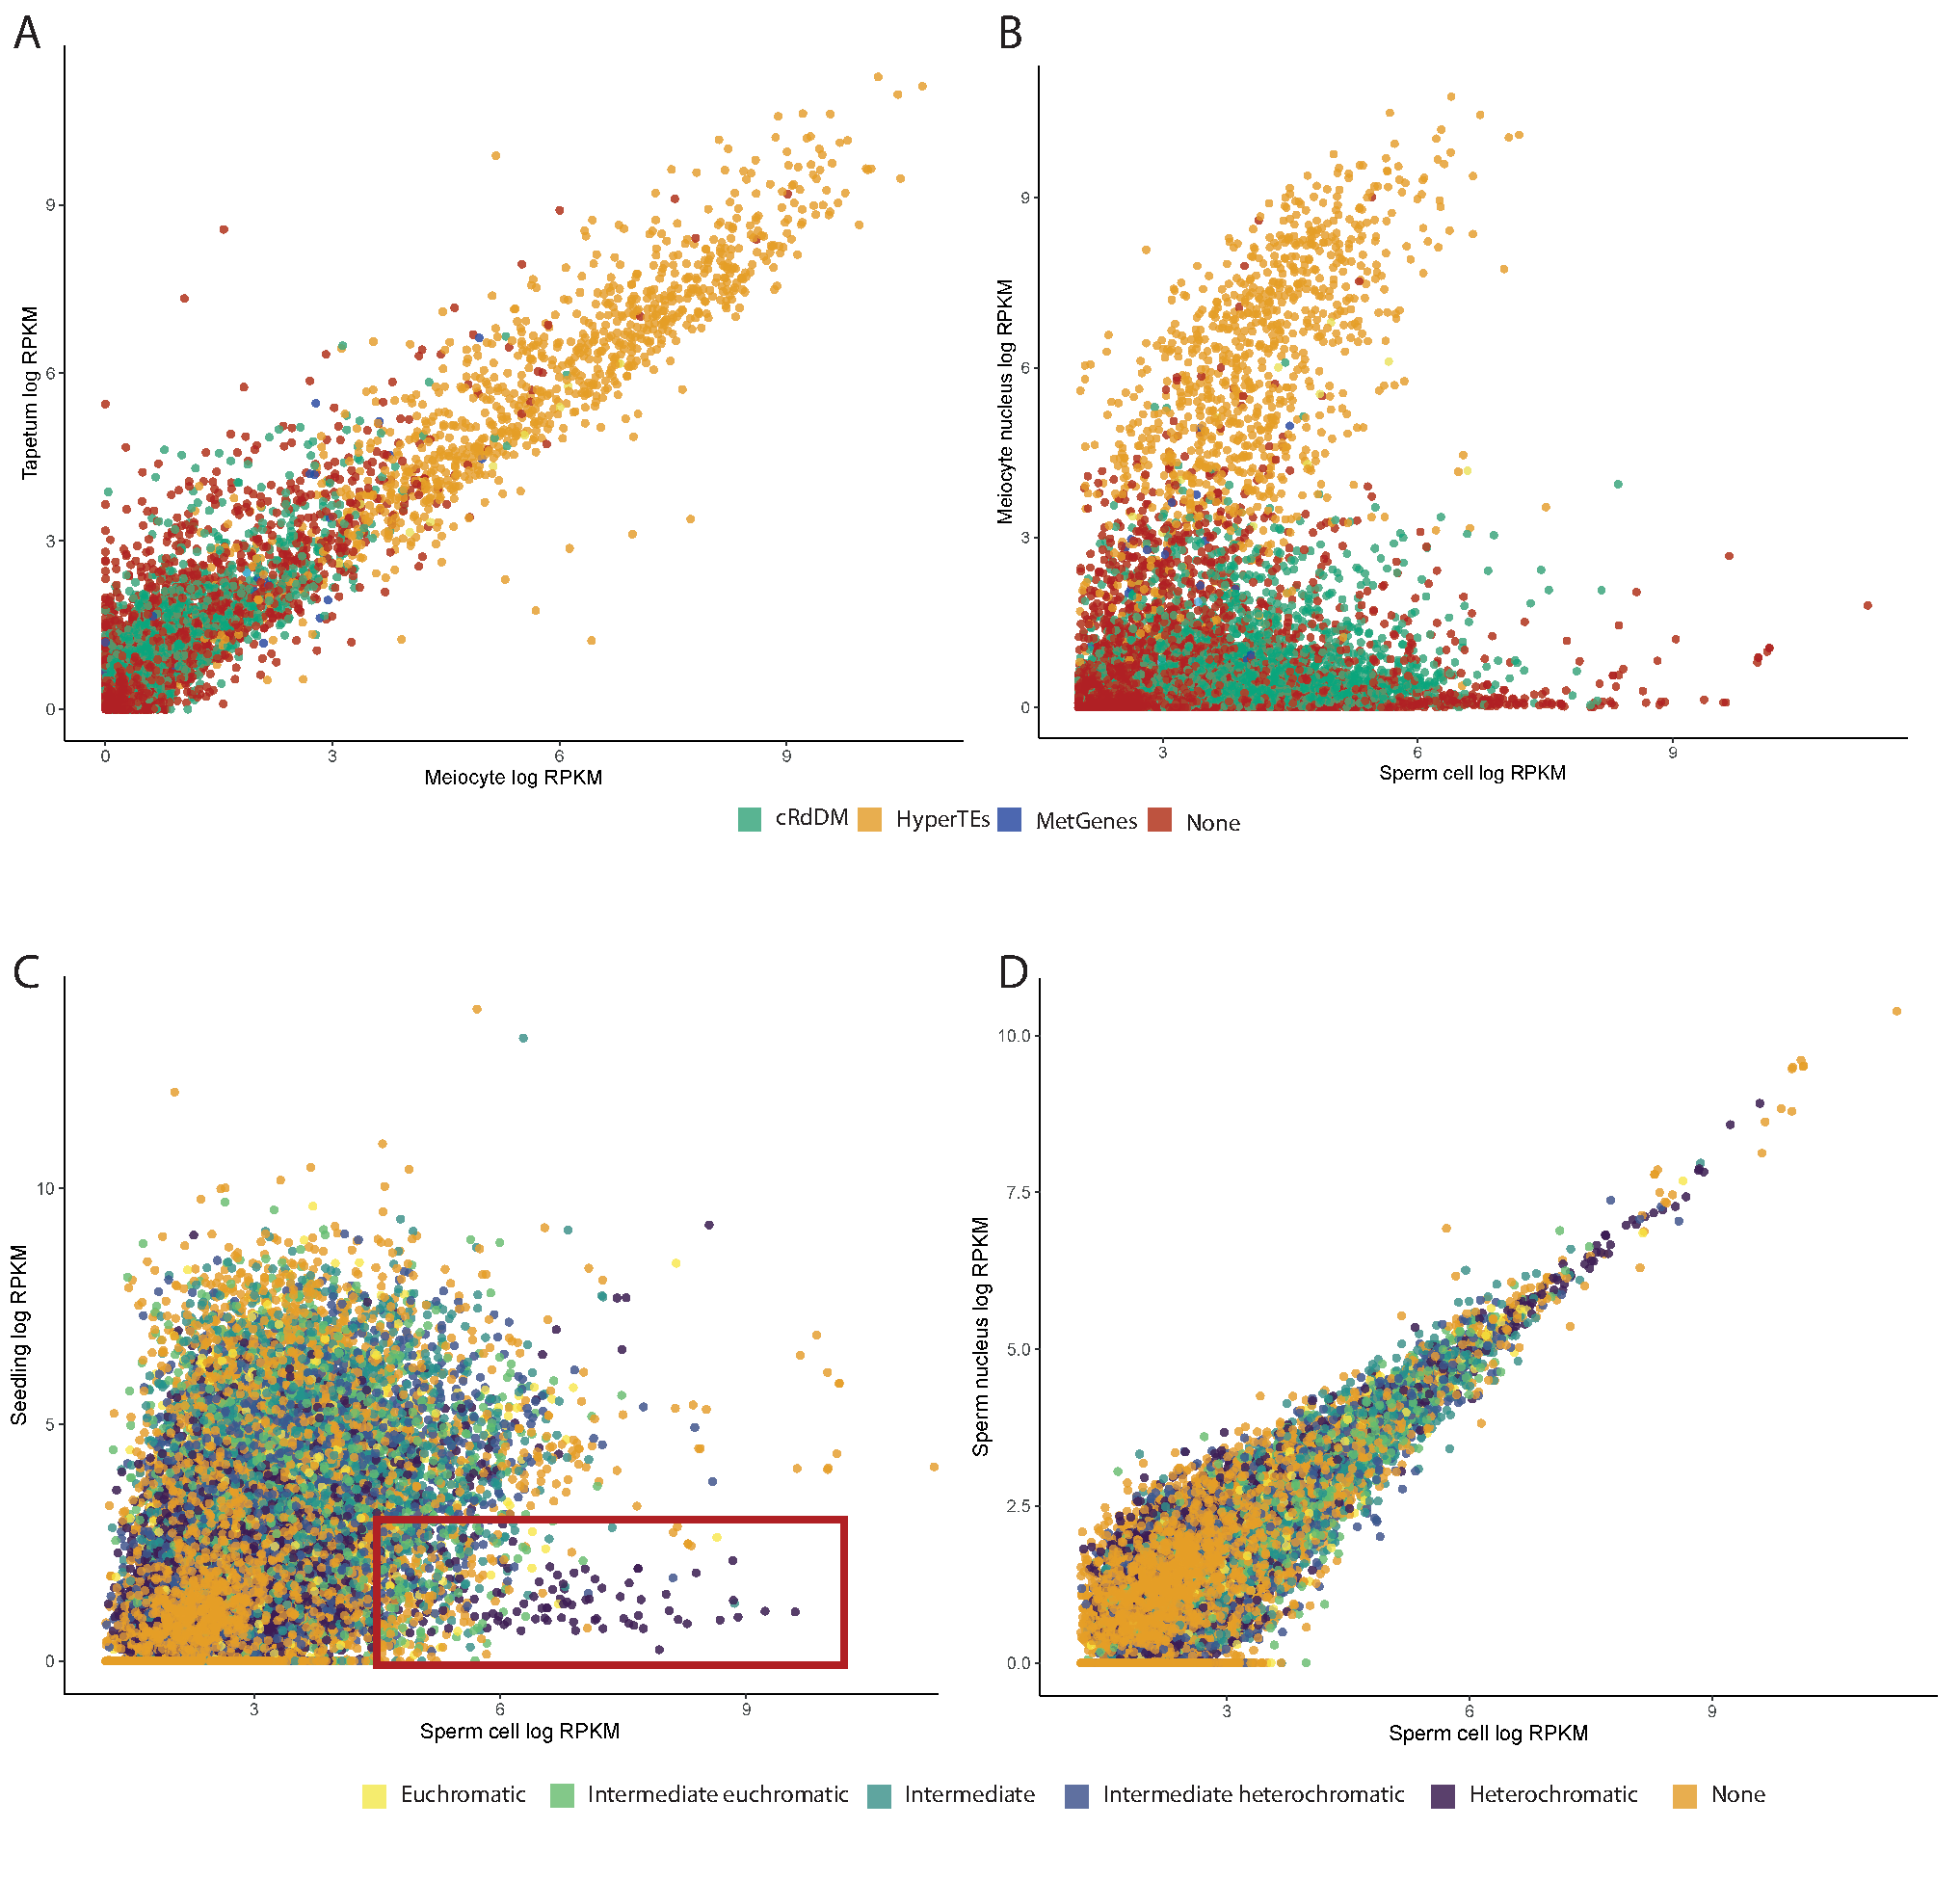
\includegraphics[width=1\textwidth]{Chapter2/Figs/Figure9_Scatterplots_HyperTEs_chromatin_SC.pdf}
\caption{\textbf{HyperTEs produce highly abundant 24nt sRNAs specifically in the meiocyte and tapetum which tapers off in the sperm cell. Loci with highly abundant 24nt sRNAs specifically in the sperm cell tend to be more heterochromatic.}}
\label{fig:scatter_SC_chromatin}
\captionsetup{font=small}
    \caption*{Correlations between 24nt sRNA abundance and the indicated cell types, highlighting (A-B) genomic features of interest and (C-D) chromatin structure. (C) Sperm cell specific heterochromatic cluster highlighed with red box. }
\end{figure}

It is crucial to investigate whether the heterochromatic sperm-specific n568 subcluster has a specific methylation pattern distinct from the whole set. We can conclude that generally, methylation in the sperm-specific sRNA clusters is consistently high, intermediate, and low in the CG CHG and CHH context throughout germline development respectively (Figure \ref{fig:SC_hetero_clusters}, dark green bars). In contrast, the n568 subcluster exhibits generally lower methylation levels compared to the full set (Figure \ref{fig:SC_hetero_clusters}, light green bars). However, when examining methylation patterns in other tissues, it becomes clear that this pattern is not exclusive to the sperm cell.

\begin{figure}[htbp!] 
\centering    
    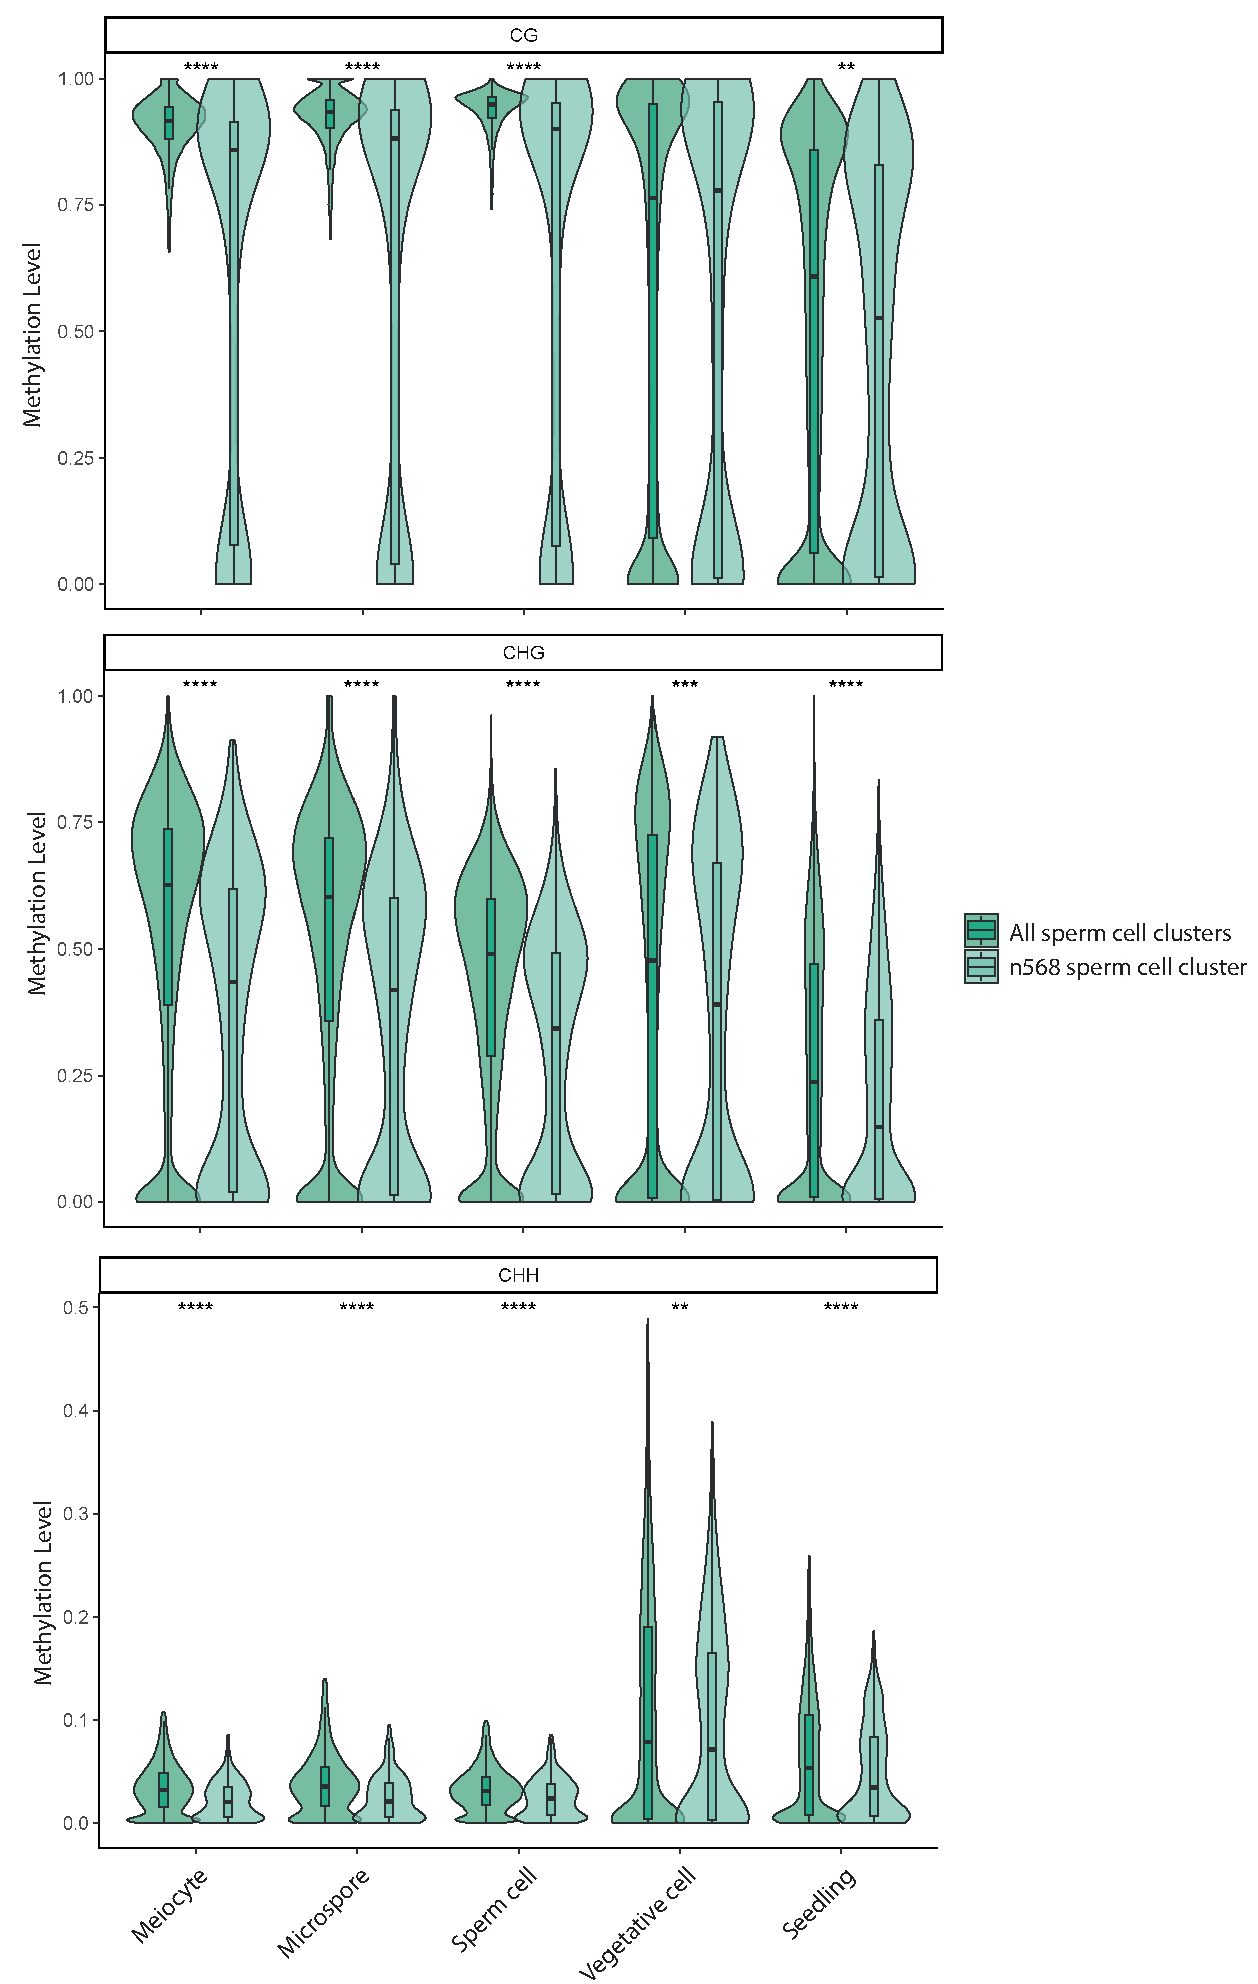
\includegraphics[width=1\textwidth]{Chapter2/Figs/Figure10_SC_hetero_clusters_methylation.pdf}
\caption{\textbf{Sperm-specific heterochromatic loci exhibit significantly lower overall methylation levels compared to the entire sperm dataset}}
\label{fig:SC_hetero_clusters}
\captionsetup{font=small}
    \caption*{CG, CHG and CHH methylation levels of all sperm clusters (dark green) and the heterochromatic 568 loci subset (light green). ***: p-value < 0.001, **: p-value < 0.01,*: p-value < 0.05}
\end{figure}

\section{A subset of MetGenes produce 24nt sRNAs and gain CHH methylation specifically in the sperm cell}

In contrast to other sex cells, about 20\% of MetGenes generate 24nt sRNAs in the sperm cell, with a subset producing sRNAs exclusively in sperm (Figure \ref{fig:hm_metgene_reactivated}, clusters 1 and 2, Figure \ref{fig:boxplot-SCPL}B). Since previous work has identified that MetGenes produce no perfect matching sRNAs in the meiocyte and tapetum\cite{RN187}, it is likely that the clusters which produce sRNAs in meiocyte and tapetum are either at HyperTE/MetGenes boundaries, or are HyperTE derived. However, the majority of sRNA producing MetGenes in the sperm cell and sperm nucleus do not overlap the same loci (Figure \ref{fig:hm_metgene_reactivated}, clusters 1 and 2: sperm specific reactivation, cluster 3: HyperTE/boundary derived meiocyte and tapetum specific clusters).

\begin{figure}[htbp!] 
\centering
    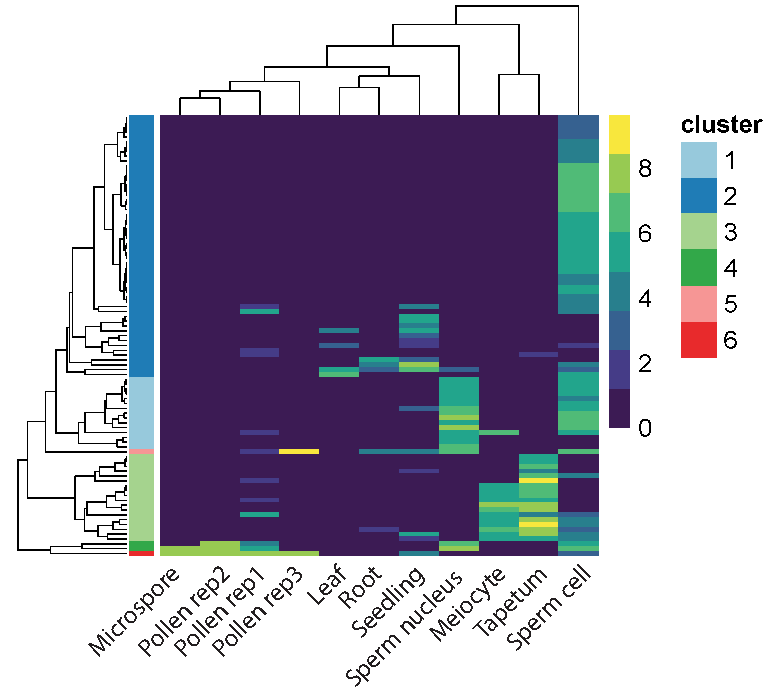
\includegraphics[width=0.8\textwidth]{Chapter2/Figs/Figure11_Reactivated_MetGenes_heatmap.pdf}
\caption{\textbf{Approximately 20\% of MetGenes produce sRNAs in the sperm}}
\label{fig:hm_metgene_reactivated}
\captionsetup{font=small}
    \caption*{Clusters 1,2: sperm specific sRNA production. Cluster 3: HyperTE/MetGene boundary derived meiocyte and tapetum specific clusters}
\end{figure}

Next, it was important to determine whether the increased sRNA production actually leads to increased DNA methylation in the sperm cell. Overall, the sperm cell-specific MetGenes exhibited higher CG and CHG methylation compared to the full set in meiocytes and microspores (Figure \ref{fig:boxplot_MetGene_methylation}A,B,D,E), and higher methylation in the CHG context in sperm. Interestingly, the only tissue where this subset showed higher CHH methylation was in the sperm cell, suggesting that renewed sRNA production at these loci also drives methylation in the sperm cell (Figure \ref{fig:boxplot_MetGene_methylation}C,F).

\begin{figure}[htbp!] 
\centering    
    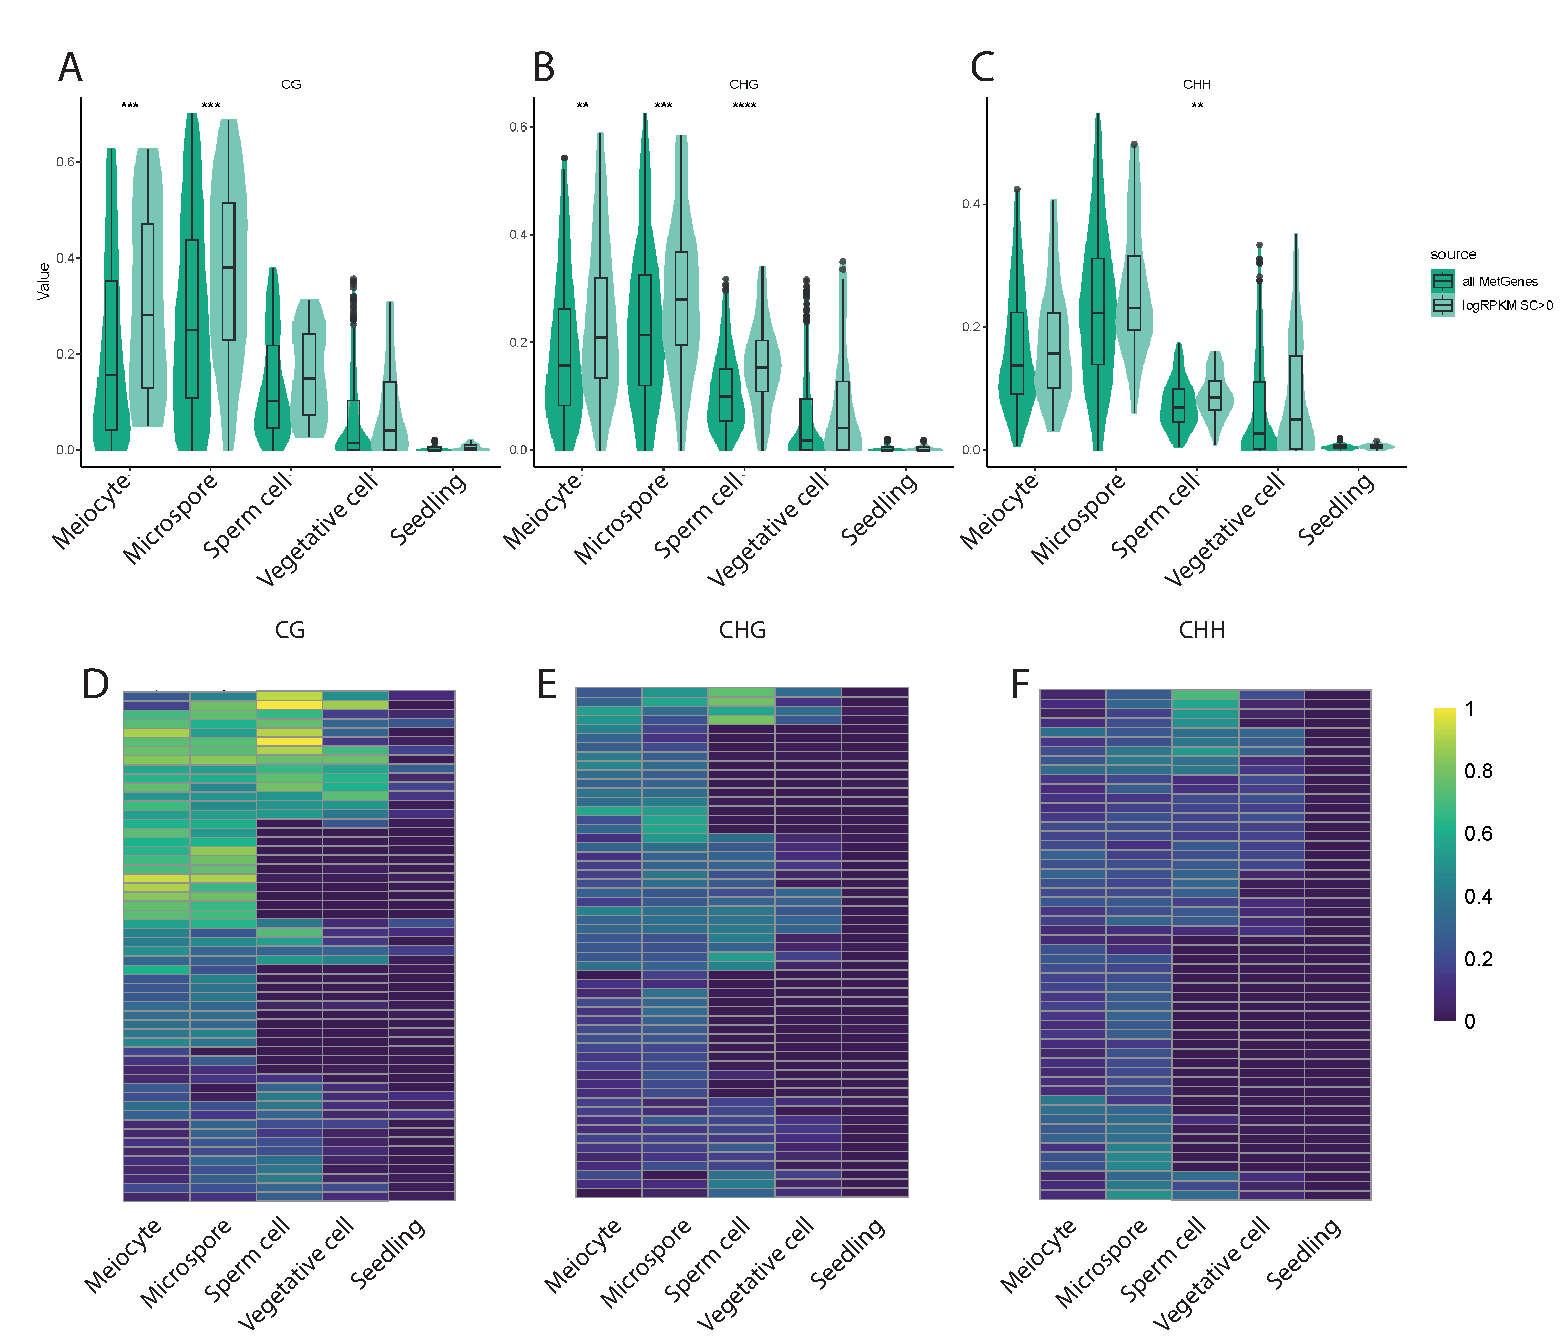
\includegraphics[width=1\textwidth]{Chapter2/Figs/Figure12_Reactivated_MetGenes_methylation.pdf}
\caption{\textbf{The reactivated MetGenes gain CHH methylation in the sperm cell.}}
\label{fig:boxplot_MetGene_methylation}
\captionsetup{font=small}
    \caption*{(Box plots of CG (A), CHG (B) and CHH (C) methylation of all MetGenes compared to the reactivated subset, in germline and somatic tissues. Heatmaps of the CG (D) CHG (E) and CHH (F) methylation MetGenes that produce sRNAs in the sperm cell. ***: p-value < 0.001, **: p-value < 0.01,*: p-value < 0.05}
\end{figure}

\section{ATGP2N TEs produce highly abundant 24nt sRNAs in sperm cells, the sperm nucleus, and pollen.}

As previously mentioned, after meiosis, HyperTE-derived sRNAs cease to be the dominant source of 24nt sRNAs in the sperm cell. Therefore it is important to analyse the landscape of 24nt sRNAs from sperm clusters overlapping TEs (Figure \ref{fig:TE_families}A). This revealed a cluster of TE families conserved across pollen, sperm cells, and sperm nuclei, which produce uniquely abundant sRNAs (Figure \ref{fig:TE_families}A, cluster 8, n=24). Within this subset, approximately 90\% of transposons belong to the LTR/Gypsy superfamily, and about 70\% are from the ATGP2 and ATGP2N families. Of these, about 40\% overlap CLSY3/4 dependent loci specifically.

\begin{figure}[htbp!] 
\centering    
    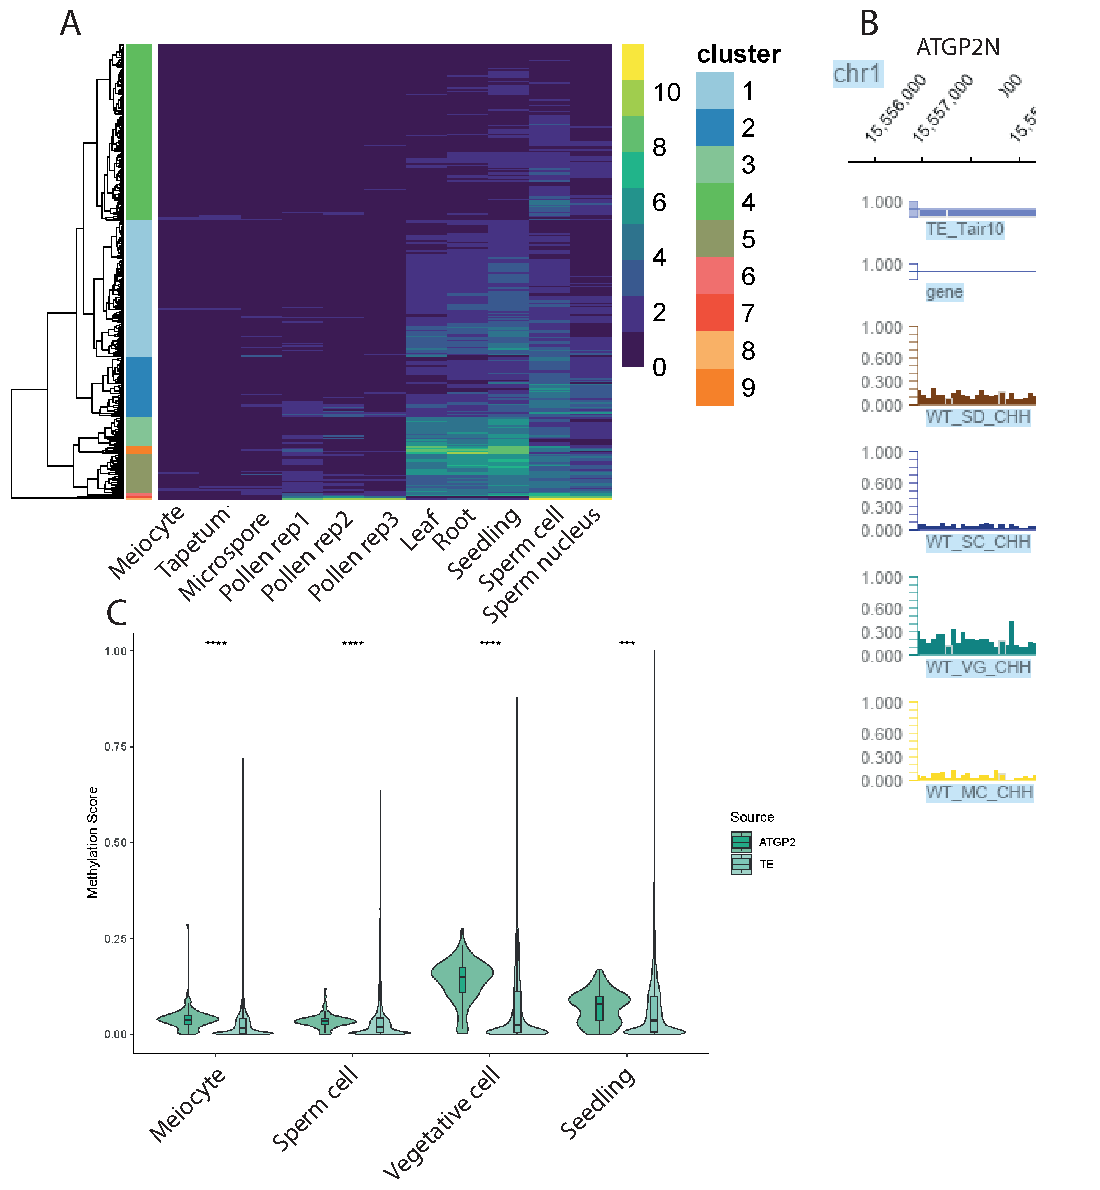
\includegraphics[width=0.8\textwidth]{Chapter2/Figs/Figure13_TE_families_heatmap.pdf}
\caption{\textbf{ATGP2N TEs produce highly abundant 24nt sRNAs in the sperm cell, sperm nucleus and pollen}}
\label{fig:TE_families}
\captionsetup{font=small}
    \caption*{(A) Heatmap showing the 24nt sRNA production of TE families in germline and somatic tissues. Cluster 9 contains the ATGP2N families.}
\end{figure}

Notably, another LTR/Gypsy transposon ATGP1 has been reported to be a direct target of RdDM in meiocytes, targeted by sRNAs produced in the tapetum, and gaining release from repression in RdDM defective mutants\cite{RN187}, specifically in the male germline.


\begin{figure}[htbp!] 
\centering    
    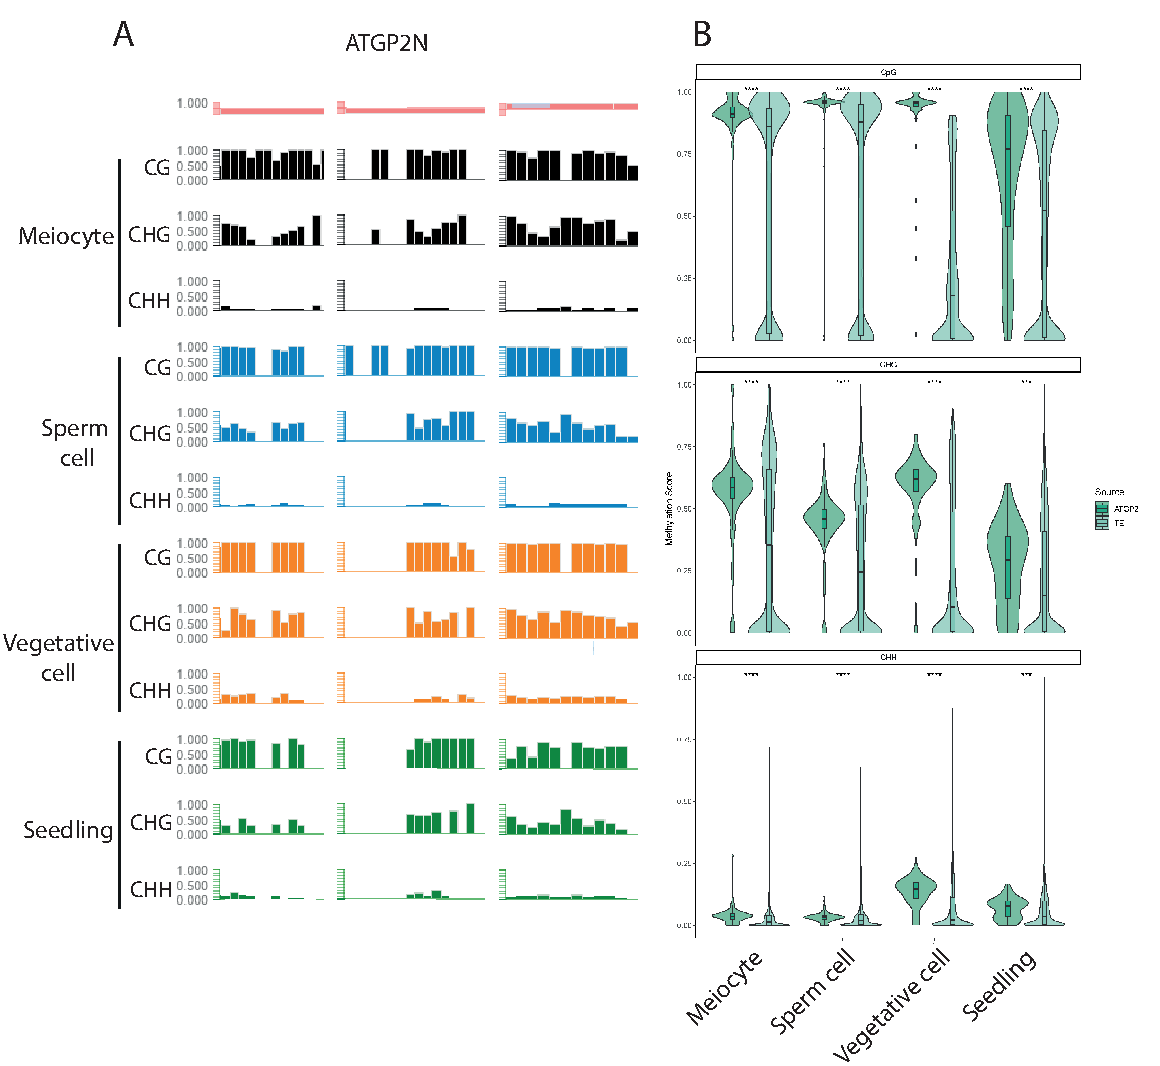
\includegraphics[width=1\textwidth]{Chapter2/Figs/Figure14_TE_methylation.pdf}
\caption{\textbf{ATGP2N TEs produce highly abundant 24nt sRNAs in the sperm cell, sperm nucleus and pollen}}
\label{fig:TE_methylation}
\captionsetup{font=small}
    \caption*{(A) Snapshot CHH methylation levels of three ATGP2N TEs which produces abundant sRNAs in the sperm. (A) Boxplots of CG, CHG and CHH methylation levels of the ATGP2 subset compared to all TEs in germline and somatic tissues. ***: p-value < 0.001, **: p-value < 0.01,*: p-value < 0.05}
\end{figure}

\clearpage

\section{Discussion}

The NRPD1 reporter line confirms the expected expression of RNA Polymerase IV in meiocyte stage anthers, namely that RNA Polymerase IV expression is restricted to the somatic tissue surrounding the sex cells and therefore 24nt sRNA production is quiescent in meiocytes (Figure \ref{fig:Pol4_anther}). At the same time, the NRPE1 reporter line also confirms the expected expression; RNA Polymerase V is expressed throughout the somatic and germline tissue, facilitating DNA methylation. This pattern aligns with the data showing similar sRNA and DNA methylation profiles in the tapetum and meiocyte, including strong germline specific methylation at 797 HyperTE loci. At the same time, specifically in the Pol IV quiescent meiocytes, HyperTE-derived 24nt sRNAs from the tapetum can target HyperTEs for methylation in the meiocytes as well as 435 \textit{de novo} genic targets (MetGenes) for methylation \cite{RN187,RN199}. 

Though generally DNA methylation levels in all sequence contexts declines through germline development overall, HyperTEs and MetGenes stay highly methylated from meiocyte to sperm \cite{RN17,RN199}. After meiosis, these results suggest that the Pol IV pathway becomes active in the germline once more, through endogenous sRNA production and DNA methylation.  The unreliable expression observed by the several NRPD1 expression lines would need further validation. This could be achieved by constructing NRPD1/NRPE1 reporter lines using a stronger fluorophore, such as tdTomato, or by confirming that the RNA levels of the reporter constructs align with the expected transcript levels of the endogenous NRPD1/NRPE1, as tissue-specific silencing may affect the transgenic reporter lines.

CLSY chromatin remodelers recruit RNA polymerase IV in a locus-specific manner to drive 24nt sRNA production in both somatic and germline tissues. CLSY1 and CLSY2 are required for the association of SHH1 with the RNA polymerase IV complex, which recognises H3K9me2 histone modifications, linking CLSY1/2-dependent loci to this histone modification \cite{RN23}. In contrast, CLSY3 and CLSY4 can recognise CG methylation to drive sRNA production at specific loci, independently of H3K9me2 \cite{RN23}. CLSY1 and CLSY2 are specifically required to produce sRNAs at cRdDM loci in leaf tissue, while CLSY3 crucial for sRNA production at siren loci in ovules and HyperTE loci in the tapetum \cite{RN162,RN23,RN187}. This tapetum-driven sRNA production also induces CHH methylation at HyperTE and MetGene loci in meiocytes, which persists throughout the germline. In fact, the production of sRNAs in the tapetum alone is sufficient to maintain HyperTE methylation in all germline tissues \cite{RN187}. In accordance with this, CLSY3 is not expressed in the meiocytes or any of the later stage sex cells. 

The CLSY1 and CLSY2 reporter lines indicate that these CLSY chromatin remodelers are not strongly expressed in maturing pollen either (Figure \ref{fig:clsy1_2_pollen}). This raises the question of how endogenous 24nt sRNA production is regulated in these germline cells. One possibility is that the reporter lines may be silenced or inaccurately expressed. To verify this, CLSY-eGFP transcript levels should be compared to RNA-seq data. RNA-seq data from our lab indicates that CLSY2 may be expressed in the vegetative cell and CLSY4 in the sperm cell (Table \ref{tab:FPKM_germ}), though these findings need further confirmation, including checks on corresponding protein expression. Additionally, some CLSY1- and CLSY4-dependent loci still appear to produce sRNAs in the sperm cell (Figure \ref{fig:clsysingle_scatters}). To conclusively determine whether any CLSY chromatin remodelers are important for sRNA production and CHH methylation in the pollen, clsy mutant sRNA data and methylation sequencing should be generated and compared with wild-type data.

In line with these findings, data analysis from the sRNA datasets seem to suggest that after meiosis, endogenous 24nt sRNA production shifts away from CLSY-mediated loci. Two hypotheses could explain this shift. First, DME-mediated hypomethylation in the vegetative cell leads to upregulated sRNA biogenesis from reactivated TEs, which in turn directs DNA methylation in the sperm cell \cite{RN57,RN39} via 21 and 22nt epigenetically active small interfering RNAs (easiRNAs). These easiRNAs are produced either by RNA polymerases II or IV and processed RDR2 or RDR6 and by DCL2/4 \cite{RN75}. Though easiRNAs are primarily 21 and 22nt in length, the discovery that RNA polymerase IV can also generate them hints at the complexity of the interplay between various RdDM variant pathways. In fact, it is already known that several other non-canonical RdDM pathways can produce and direct 24nt sRNAs into the canonical RdDM pathway. One such pathway bypasses Pol IV-RDRs entirely, where double-stranded Pol II-derived transcripts (such as inverted repeats or microRNA precursors) are directly cleaved by DCL proteins to produce sRNAs \cite{RN269}. The DCLs compete for these transcripts and produce 21-24nt sRNAs \cite{RN268}), and the 24nt sRNAs can feed into the Pol V pathway via AGO4 either in \textit{cis} or at other similar loci in \textit{trans} \cite{RN270,RN269}. Alternatively, post-transcriptional gene silencing (PTGS) has also been linked to the RdDM pathway. In this pathway, dsRNA is first produced by PTGS via Pol II and RDR6 which is then cleaved by either DCL2/4, or DCL3 to produce 21,22 or 24nt sRNAs respectively, in a hierarchical manner \cite{RN267}, which can be loaded onto AGO proteins and feed into the Pol V pathway this way \cite{RN133}. 

Several accessory proteins are involved in the RdDM pathway \cite{RN33}, many of which have paralogs in \textit{Arabidopsis}. While some of these proteins may have redundant functions, RNA-seq data generated by members of our lab shows that specific Pol IV and Pol V accessory proteins are expressed at specific developmental stages in the male sexual lineage. I would like to highlight three specific examples and discuss their roles. 

 First, a paralog of SPT5L/KTF1, which recruits AGO proteins through an AGO hook motif \cite{RN121,RN273}  and interacts with NRPE1 \cite{RN271,RN272}, is notably upregulated in meiocytes and pollen. Second, RNA polymerase V transcription is facilitated by the DDR complex, a key component of which, a DRD1 homolog, is specifically upregulated in the meiocyte (Table \ref{tab:FPKM_germ}). Finally, the MORC protein family, which consists of ATPases involved in chromatin compaction and transcriptional gene silencing in mammals, also plays a crucial role in the canonical RdDM pathway in plants. MORC proteins co-localise to sites of RdDM and are important for the establishment of RdDM. One paralog, MORC5 is specifically upregulated in the meiocyte (Table \ref{tab:FPKM_germ}) and has been previously shown to be specifically expressed in the pollen \cite{RN274}, while MORC4 is also upregulated in the meiocyte, pollen and embryo (Tables \ref{tab:FPKM_germ} and \ref{tab:FPKM_soma}). These observations hint at possible candidates that could contribute to tissue-specific non-canonical RdDM pathways in the male sexual lineage.

Given the critical importance of genome integrity in reproductive cells, the precise regulation and silencing of TEs are essential. In accordance with this, 568 loci with abundant 24nt sRNAs also have high H3K9me2 methylation, which is associated with heterochromatic regions, however, these loci are not associated with increased CG, CHG or CHH methylation levels when compared to the whole set (Figures \ref{fig:scatter_SC_chromatin} \ref{fig:SC_hetero_clusters}. This may suggest that this subset represent TEs that are activated in the vegetative cell, which are situated in pericentromeric regions, enriched in H3K9me2, and produce 24nt sRNAs that target DNA methylation in sperm cells \cite{RN278}. Nevertheless, further careful study is necessary to determine the specific significance of this group of TEs and to clarify whether they overlap with the heterochromatic TEs activated in the vegetative cell.

The LTR/Gypsy TE family ATGP1 has previously been shown to be specifically active in reproductive cells of RdDM mutants \cite{RN187}. Investigating the 24nt sRNA landscape at TE loci identified another LTR/Gypsy TE family, ATGP2N, which produce abundant sRNAs specifically in the sperm cell (Figure \ref{fig:TE_families}). ATGP2N has previously been reported to gain chromatin accessibility and be transcriptionally upregulated in \textit{met1} mutants. In this study ATGP2N was part of a subset of TEs that gained chromatin accessibility and increased in transcription as well as an increase in the production of 21nt sRNAs in the inflorescences of \textit{met1} mutants. The other groups gained accessibility but had no change in transcription or sRNA production, one already being highly expressed in wild type plants, and the other remaining repressed with respect to transcription and sRNA production even with increased chromatin accessibility\cite{RN184}. Although CHH methylation levels of TEs  both germline and somatic tissues were generally low, the ATGP2N family had slightly increased CHH methylation in all tissues, most notably in the vegetative cell (Figure \ref{fig:TE_methylation}B and C). Several explanations could account for these findings. 

Firstly, as around 40\% of these ATGP2N loci overlap CLSY3/4 dependent loci, it is possible that these chromatin remodelers are responsible for the cell-specific silencing of these TEs in the sperm cell. An important question to address empirically is whether, in addition to the 21 and 22nt easiRNAs, 24nt sRNAs produced in the hypomethylated vegetative cells can direct methylation in the sperm cells, similar to how tapetal cells mediate methylation at specific loci. Secondly, another potential explanation for this sRNA and methylation pattern is related to the general observation that most TEs are more hypomethylated in the vegetative cell compared to the sperm cell, which leads to the production of abundant easiRNAs that direct RdDM in sperm.  However, since ATGP2N exhibits increased CHH methylation in the vegetative cell compared to the sperm cell, it is plausible that the abundant 24nt sRNAs detected in the sperm cell are produced through the non-canonical PolII-RDR6 or PolII-DCL3 RdDM pathways, due to ATGP2N reactivation specifically in the sperm cell. To verify these hypotheses, it will be necessary to examine ATGP2N expression levels in the germline of wild-type and RdDM mutants, as well as analyse 24nt sRNA production and CHH methylation in clsy3/4 double mutants.

Notably, around 20\% of MetGenes produce perfect-matching 24nt sRNAs uniquely in the sperm cell (Figures \ref{fig:PLvSC_cRdDMs}, \ref{fig:hm_metgene_reactivated}) and these genes specifically gain CHH methylation in the sperm cell (Figure \ref{fig:boxplot_MetGene_methylation}C). This could be an off-target effect of sRNAs produced in the vegetative cell due to hypomethylation of TEs, a relationship that warrants further investigation. Alternatively, this CHH methylation gain may have biological significance. While CHH methylation is often linked to transcriptional repression, this is not always the case.  For example, gene body methylation near transposon-gene boundaries is associated with transcriptionally active genes in maize \cite{RN277}. Additionally, the loss of RdDM-directed gene body methylation of MetGene MPS1 has been proven to cause mis-splicing and disrupt meiosis \cite{RN199}.Among the MetGenes producing 24nt sRNAs in the sperm cell are VIM2 and VIM4. The VIM proteins are required for maintaining CG methylation by recruiting MET1 to hemimethylated CG sites \cite{RN276}. In addition, VIM5 was identified as one of few paternally imprinted genes in \textit{Arabidopsis} and is involved in mediating CG methylation in the endosperm \cite{RN275}. RNA-seq data provides evidence that VIM proteins are specifically upregulated in the sperm cell and VIM1 specifically upregulated in the vegetative cell (Table \ref{tab:VIM_expression}), suggesting a potential connection between tissue-specific gene body CHH methylation and transcriptional regulation. This differential expression may play a crucial role in maintaining epigenetic control and ensuring correct gene expression and TE silencing in these important tissues.

Together, these observations highlight that, in addition to producing 24nt sRNAs from cRdDM loci, sperm cells display a unique sRNA profile  distinct not only from earlier germline cells and somatic tissues but also, to some extent, from vegetative cells. This difference may be driven by non-canonical RdDM pathways and may shift away from CLSY chromatin remodelers regulating RdDM after meiosis. The tissue-specific expression of several key RdDM components in the male sexual lineage suggests potential mechanisms that could allow mismatch-targeted DNA methylation in meiocytes and underscores the significance and complexity of non-canonical RdDM pathways active during post-meiotic male sexual development.

\clearpage

\section{Materials and Methods}

\subsection{Plant materials and growth conditions}

\textit{Arabidopsis thaliana} plants were grown in 16h light/8h dark conditions, in 21°C, 70\% humidity in a controlled environment chamber on germination medium (GM) without glucose supplementation. The following lines have been grown: Col-0 wild type plant for the microspore and pollen sRNA sequencing libraries. For the anther imaging experiments, the transgenic reporter lines pCLSY1::CLSY1-eGFP (clsy1), pCLSY2::CLSY2-eGFP (WT), pCLSY3::-CLSY3-Venus (clsy3) and pCLSY4::CLSY4-eGFP (clsy4), pNRPD1::NRPD1-eGFP (WT), pNRPE1::NRPE1-eGFP (WT) were used with pAGO4::AGO4-Venus or ), pCLSY3::-CLSY3-Venus (clsy3) for a positive control.

\subsection{Microscopy}

Meiocyte and microspore stage anthers were dissected using a Leica dissecting microscope on 0.8\% agar and vacuum infiltrated in DAPI buffer (Galbraith’s buffer (45 mM MgCl2-6H2O, 30 mM trisodium citrate, 20 mM MOPS, pH 7.0), 1 µg/mL DAPI, and 0.01\% [v/v] Triton X-100) briefly, then imaged using imaging spacers (SecureSealTM Grace BioLabs). Individual microspores and pollen were imaged after isolation from unopened flower buds and opened flowers respectively, by collecting ~500 µL of flower buds into DAPI buffer, briefly vortexing and pelleting cells. All samples were imaged using Leica Stellaris 8 and Leica SP8X confocal microscopes.

\subsection{Isolation of microspores and pollen using fluorescence activated cell sorting}

\textit{Arabidopsis thaliana} microspores were isolated by manually collecting microspore stage flower buds, using the morphology described previously \cite{RN86}. The buds were collected into 1.5mL microcentrifuge tubes and suspended in PEB (10 mM CaCl2, 2 mM MES, 1 mM KCl, 1\% H3BO3, 10\% Sucrose, pH 7.5) buffer. The microspore cells were isolated as described previously \cite{RN140}. Briefly, the buds were gently ground in a clean pestle and mortar in PEB buffer and filtered through Miracloth (Merck-Millipore 475855) into a 1.5mL Eppendorf tube. This crude fraction was centrifuged for 5 minutes at 800g to gently pellet the microspore cells. The pellet was resuspended in 500µL PEB and sequentially filtered through 30µm and 20µm mesh filters (CellTrics®).

The fraction was separated using fluorescence-activated cell sorting (FACS) on a BD FACSMelody cell sorter (Beckton Dickinson) into TRI reagent (Zymo Research). The purity of the sorted cells was inspected using a widefield microscope.

Sperm cells were isolated as previously described \cite{RN140,RN141} except the sperm cell release step was repeated 4 times to maximise sperm cell release from pollen grain. Sperm cells were stained using SYBR green and SITOX orange and sperm cells and nuclei were sorted into TRI reagent (Zymo Research).

\subsection{sRNA sequencing}

RNA was released from isolated microspores by vortexing the samples with RNase free glass beads (Sigma-Aldrich) for 4 minutes before proceeding with RNA isolation. RNA was isolated from all samples using the Direct-zol™ RNA kit (Zymo Research, CN: R2061).

2 replicates of sRNA sequencing libraries were constructed per cell type (microspore, sperm cell, sperm nuclei) using the RealSeq®-biofluids NGS Library Preparation Kit for miRNAs and small RNAs. For the three library types the number of cells used for each replicate were as follows: 300 000 cells for microspore, 600 000 cells for sperm cells, and 1 500 000 cells for sperm nuclei.

Briefly, the RealSeq® adapters were ligated and blocked, then the sample was circularised, and the adapter dimers were removed. Then reverse transcription was performed as well as PCR amplification and size selection to end up with the final library.

Further, gel separation  and purification was performed to enrich the sRNA libraries for the desired fragment lengths (20-30 nucleotides long) as described previously \cite{RN187}. The libraries were ran on Novex TBE 6\% gels (Invitrogen, CN: EC6265BOX) along with a custom RNA ladder consisting of bands that were 146bp and 161bp in length. 

The gel was run for 45 mins with 120V and then stained using ethidium bromide. The gel was illuminated with UV light and the area between the two bands were then cut out using a clean razor blade and the gel slice was weighed. 2 volumes of elution buffer (0.5 M ammonium acetate, 10 mM magnesium sulfate, 1 mM EDTA (pH 8.0), 0.1\% SDS) was added to the gel slice. The sample was incubated at 37°C on a rotary platform (1000 RPM) for 4 hours. 

The sample was then centrifuged at 12000g for 1 minute at 4°C in a microcentrifuge. The supernatant was transferred into a fresh 1.5mL Eppendorf tube. An additional 200µL of elution buffer was added to the polyacrilamide gel fragment, vortexed, re-centrifuged and the two supernatants were combined. Any remaining fragments of polyacrilamide were removed  by passing the supernatant through a plastic column containng cellulose acetate filters. Two volumes of cold absolute ethanol was added and the solution was incubated on ice for 30 minutes. The DNA was recovered by centrifugation at 12000g got 10 minutes at 4°C. The pellet was dried and resuspended in 200µL TE buffer (10mM Tris-HCl, 1mM EDTA, pH 7.6) and 25µL of 3M sodium acetate (pH 5.2) was added. The precipitation step was repeated, the pellet was rinsed with 70\% ethanol and thoroughly dried before resuspending in TE buffer to a final volume of 30µL. The sample was incubated at 4°C overnight to redissolve the DNA.

The concentration and size distribution of purified sRNA libraries were determined using  High Sensitivity DNA Chips (Agilent Technologies, CN: 5067-5594).

The sRNA libraries were sequenced using a NextSeq 500 (Illumina).

\subsection{Bioinformatics and data analysis}

Adaptor trimming and filtering of reads that are 18nt to 28nt in length was performed on the raw sequencing data using Cutadapt \cite{RN88} v1.9.1). These reads were mapped to the Arabidopsis thaliana reference genome TAIR10 using Bowtie \cite{RN89}. 24nt clusters were extracted and loci were kept that overlapped previously determined non-overlapping genomic features of interest such as canocical RdDM loci (9629 loci), HyperTEs (797 loci), MetGenes (435 loci), transposons (TEs), genes17,20, and H3K9me2 enriched loci. These overlapping feature files were produced using BEDtools (v2.27.0) \cite{RN90}. 24nt sRNA clusters were extracted using ShortStack \cite{RN142} (n = 45639). To firstly identify true 24 nucleotide clusters, the ShortStack clusters from the two replicates were filtered to keep clusters where the predominant read length was 24 nucleotides long, where log2(RPKM+1) 24nt sRNA > log2(RPKM+1) 25nt sRNA +2 and that were >99bp (n = 34032).

Following this general filtering step, sperm cell specific clusters were identified where:
log2(RPKM+1) 24nt sperm cell sRNA > 0 \& where:
log2(RPKM+1) 24nt sperm cell sRNA - log2(RPKM+1) 24nt (other tissues: tapetum, meiocyte, microspore, root seedling and leaf) sRNA > 3 which resulted in 513 loci.

The euchromatic/heterochromatic annotation was allocated based on data from reference \cite{RN183} and classified into 5 chromatin states based on H3K9me2/H3: euchromatic (less than 0.6), intermediate euchromatic (bw. 0.6 and 0.9), intermediate (bw 0.9 and 1.4), intermediate heterochromatic (bw. 1.4 and 2.6), heterochromatic (above 2.6). 

 Figures were plot using ggplot2 and pheatmap packages in R (v4.0.3). Please find all scripts used at \href{https://github.com/talasjudit}{my personal GitHub page}.


%!TEX root = ../thesis.tex
%*******************************************************************************
%****************************** Third Chapter **********************************
%*******************************************************************************
\chapter{The dynamic sRNA profile and inheritance of paternal epigenetic modifications post-fertilisation in the embryo of \textit{Marchantia polymorpha}}

% **************************** Define Graphics Path **************************
\ifpdf
    \graphicspath{{Chapter3/Figs/Raster/}{Chapter3/Figs/PDF/}{Chapter3/Figs/}}
\else
    \graphicspath{{Chapter3/Figs/Vector/}{Chapter3/Figs/}}
\fi


\section{Abstract}

Global cytosine methylation reprogramming has recently been reported in the male sexual lineage of Marchantia polymorpha. During spermiogenesis, global 5mC expansion occurs followed by the expansion of 4mC onto CG sites, a DNA modification previously only described in bacteria and archaea. Following fertilisation, the mature embryo loses this epigenetic mark, so it’s crucial to understand whether 4mC is maintained or passively lost after fertilisation.


\section{Introduction}

Recently, our group has shown that during spermatogenesis, there extensive DNA methylation reprogramming in Marchantia. As well as the deposition of 5-methylcytosine (5mC), there is an additional wave of DNA methylation reprogramming whereby N4-methylcytosine (4mC) - an epigenetic modification previously only found in prokaryotes – is deposited at the majority of CG cites across the genome \citep{RN189}. 

\begin{figure}[htbp!] 
\centering    
    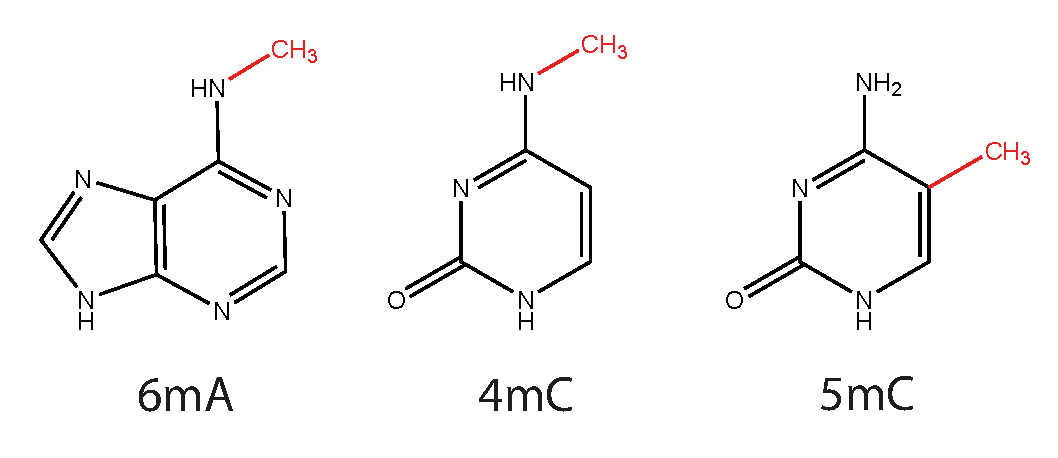
\includegraphics[width=0.5\textwidth]{Chapter3/Figs/Intro/base_mods.pdf}
\caption{}
\label{fig:base_mods}
\captionsetup{font=small}
    \caption*{}
\end{figure}

\begin{figure}[htbp!] 
\centering    
    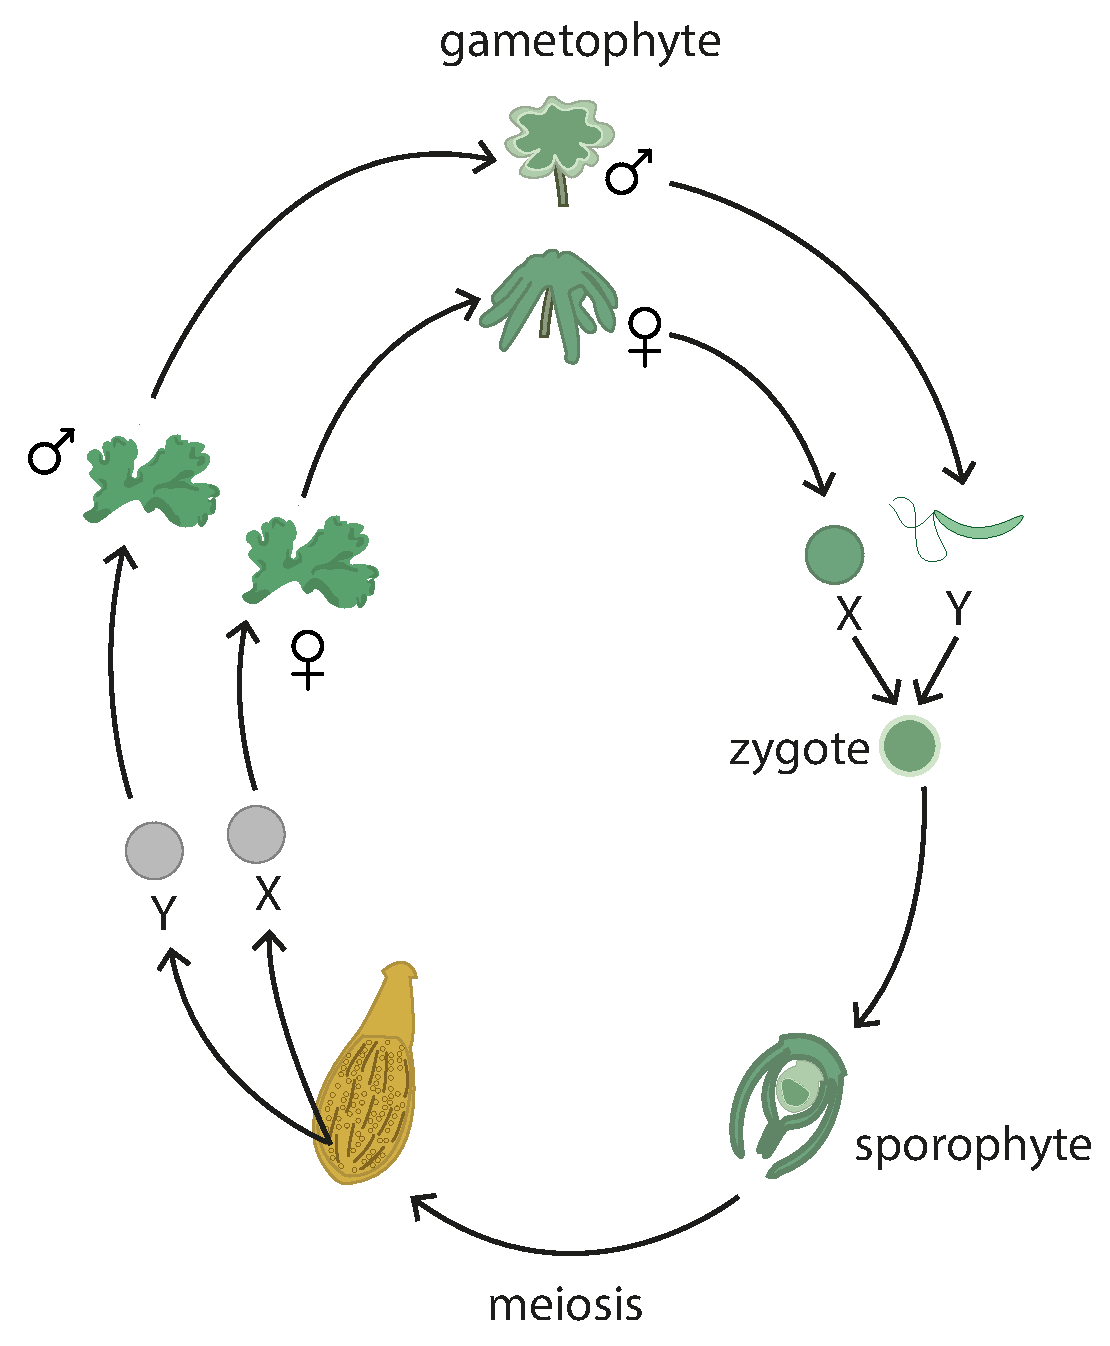
\includegraphics[width=0.5\textwidth]{Chapter3/Figs/Intro/Marchantia_lifecycle.pdf}
\caption{}
\label{fig:Mp_lifecycle}
\captionsetup{font=small}
    \caption*{}
\end{figure}

\begin{figure}[htbp!] 
\centering    
    \includegraphics[width=0.7\textwidth]{Chapter3/Figs/Intro/Embryo_development.pdf}
\caption{}
\label{fig:Mp_embryo_dev}
\captionsetup{font=small}
    \caption*{}
\end{figure}
\begin{figure}[htbp!] 
\centering    
    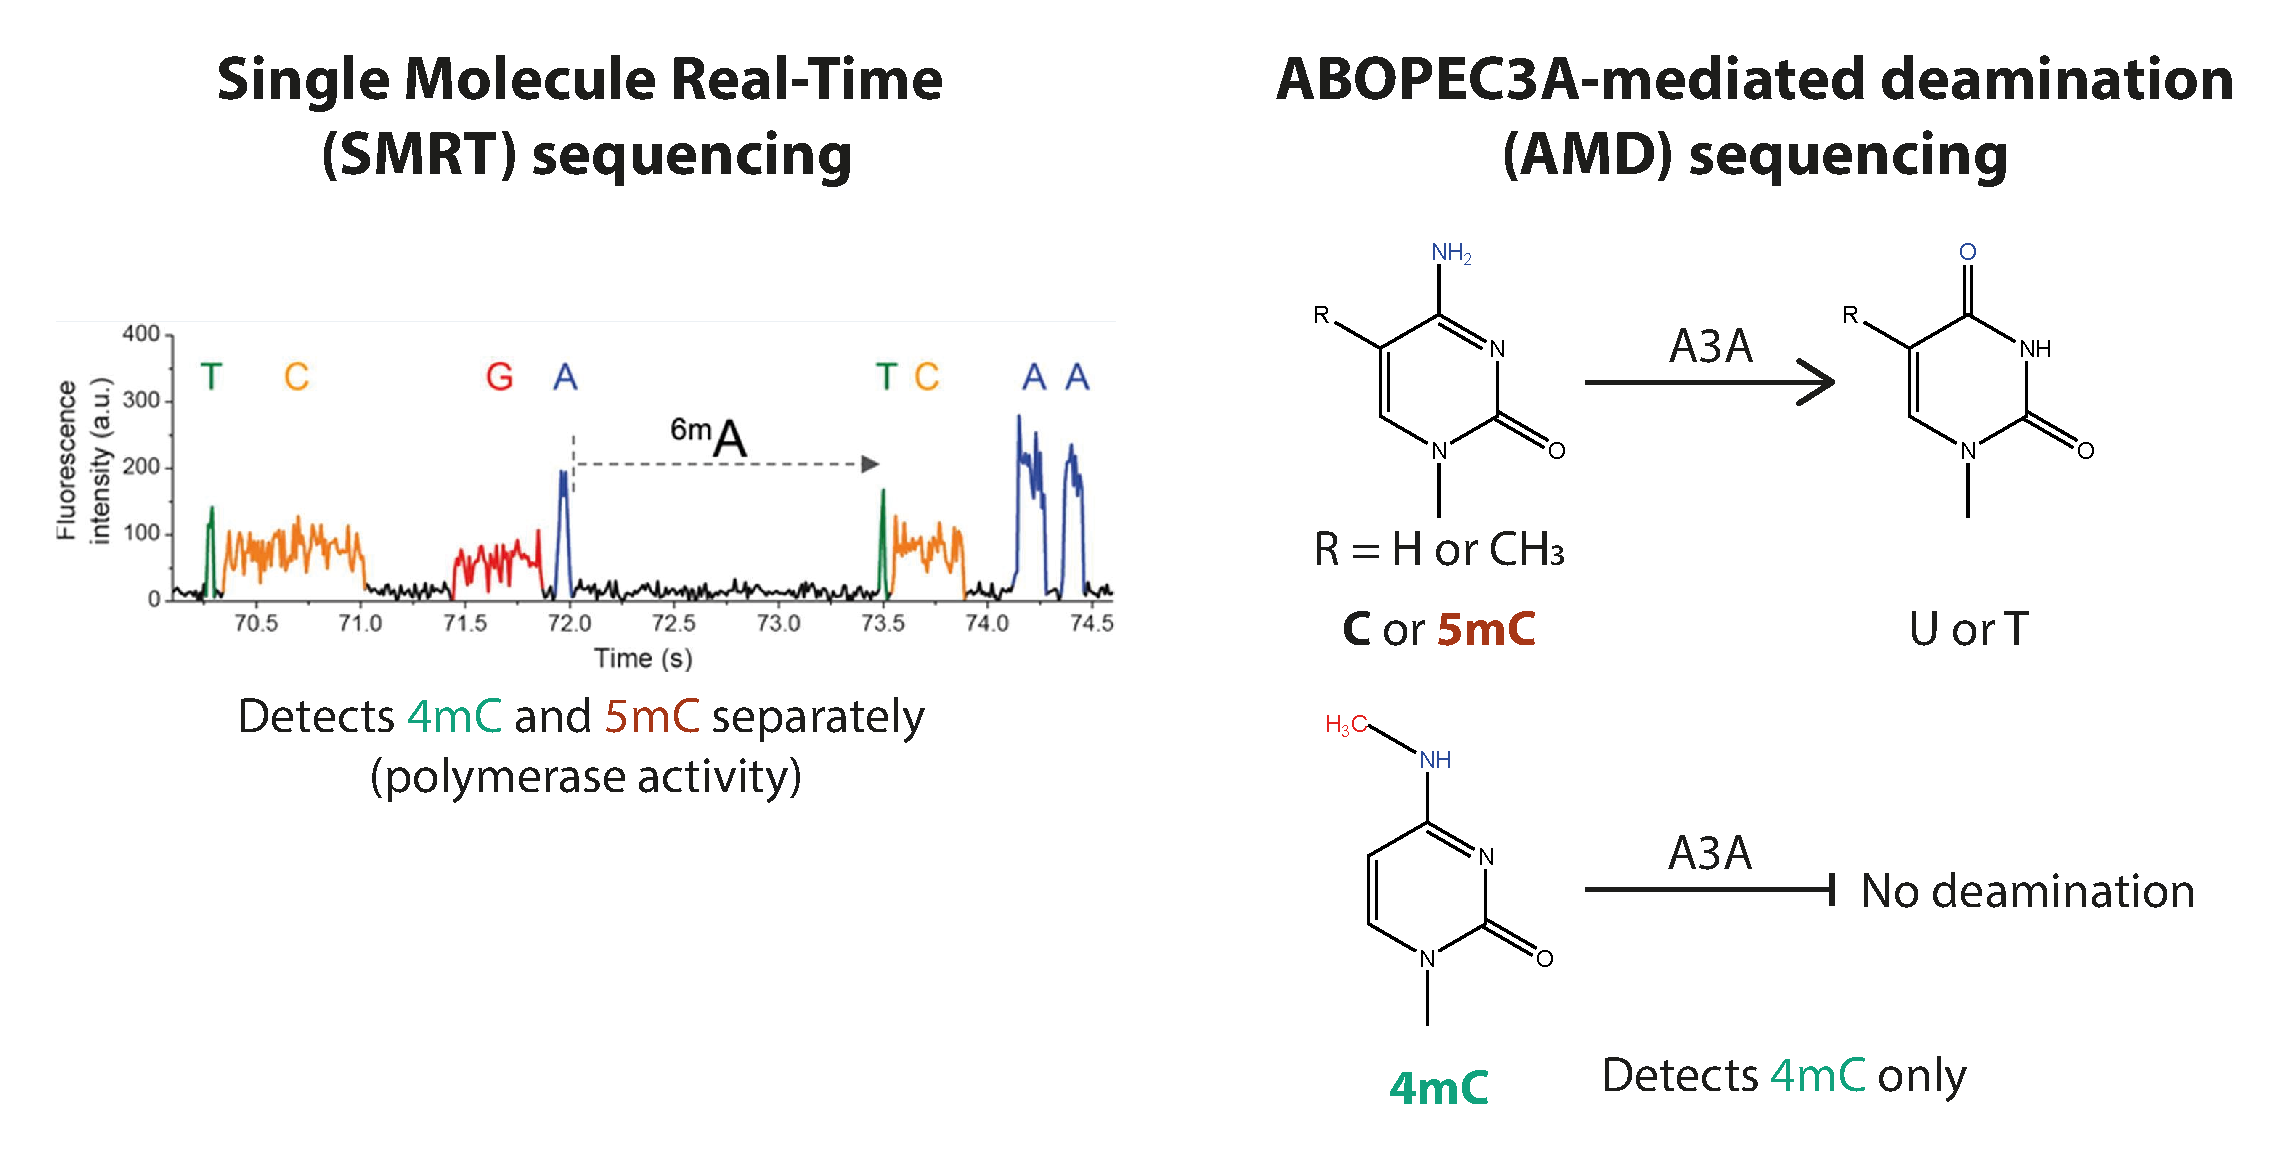
\includegraphics[width=1\textwidth]{Chapter3/Figs/Intro/Sequencing_techs.pdf}
\caption{}
\label{fig:Mp_seq_techs}
\captionsetup{font=small}
    \caption*{}
\end{figure}

\begin{figure}[htbp!] 
\centering    
    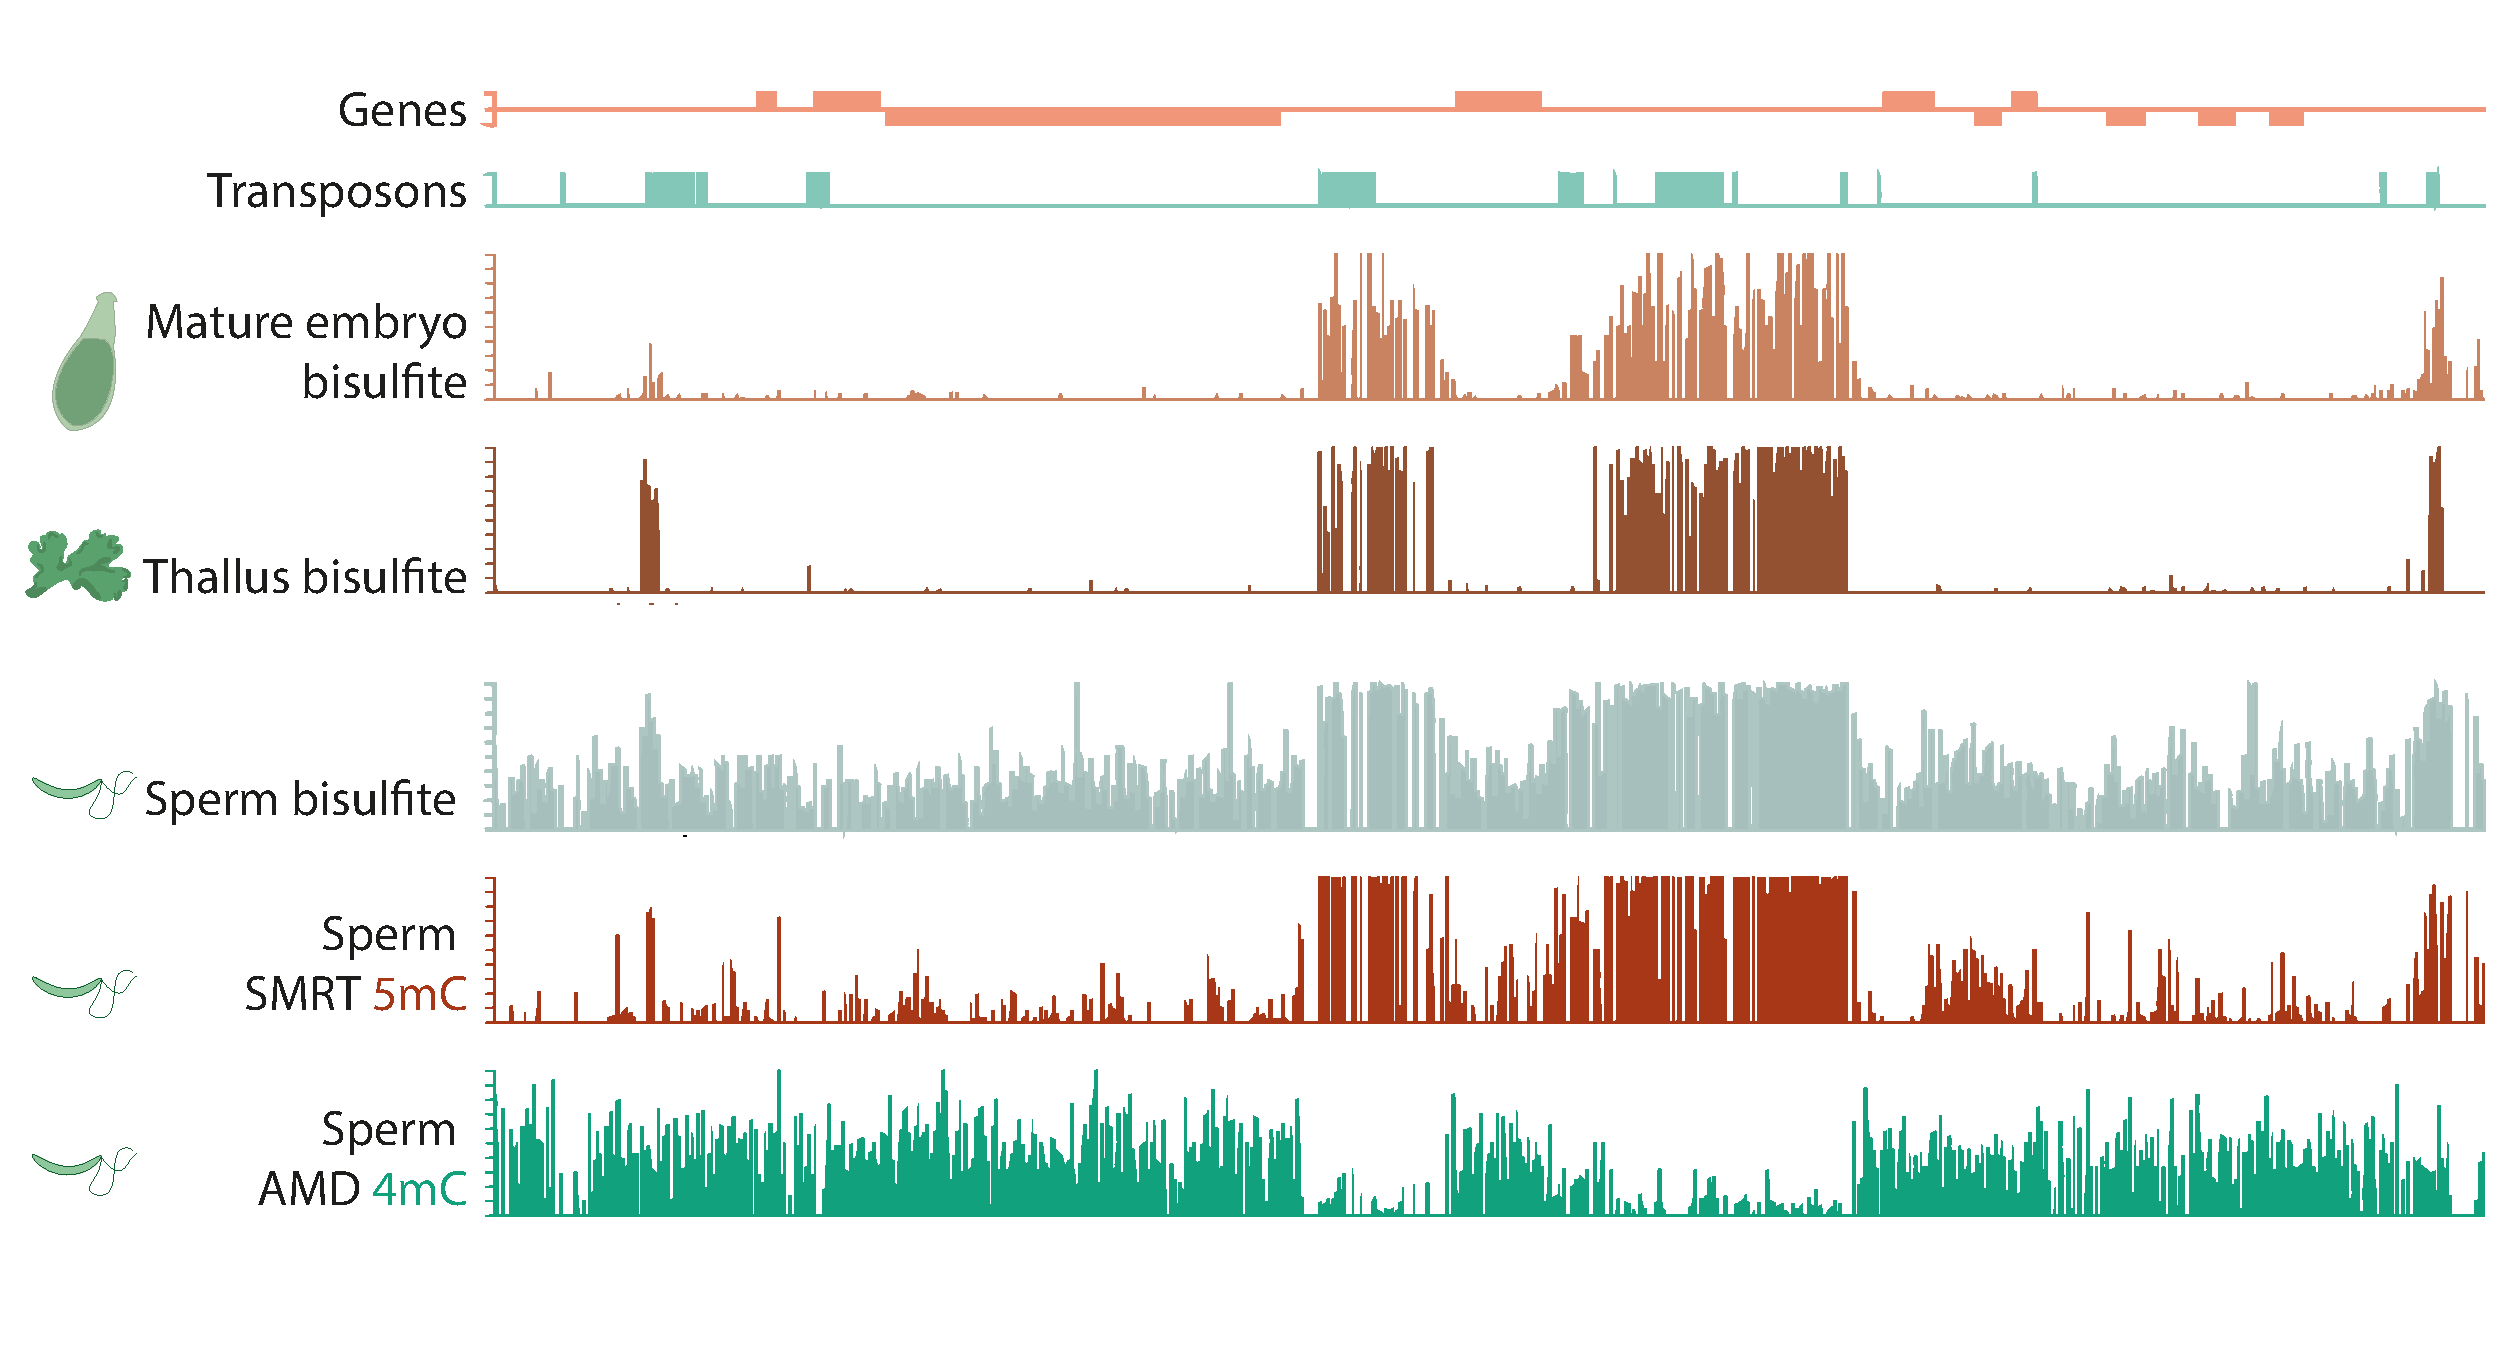
\includegraphics[width=1\textwidth]{Chapter3/Figs/Intro/Marchantia_germline_seq.pdf}
\caption{}
\label{fig:Mp_germline-seq}
\captionsetup{font=small}
    \caption*{}
\end{figure}

\begin{figure}[htbp!] 
\centering    
    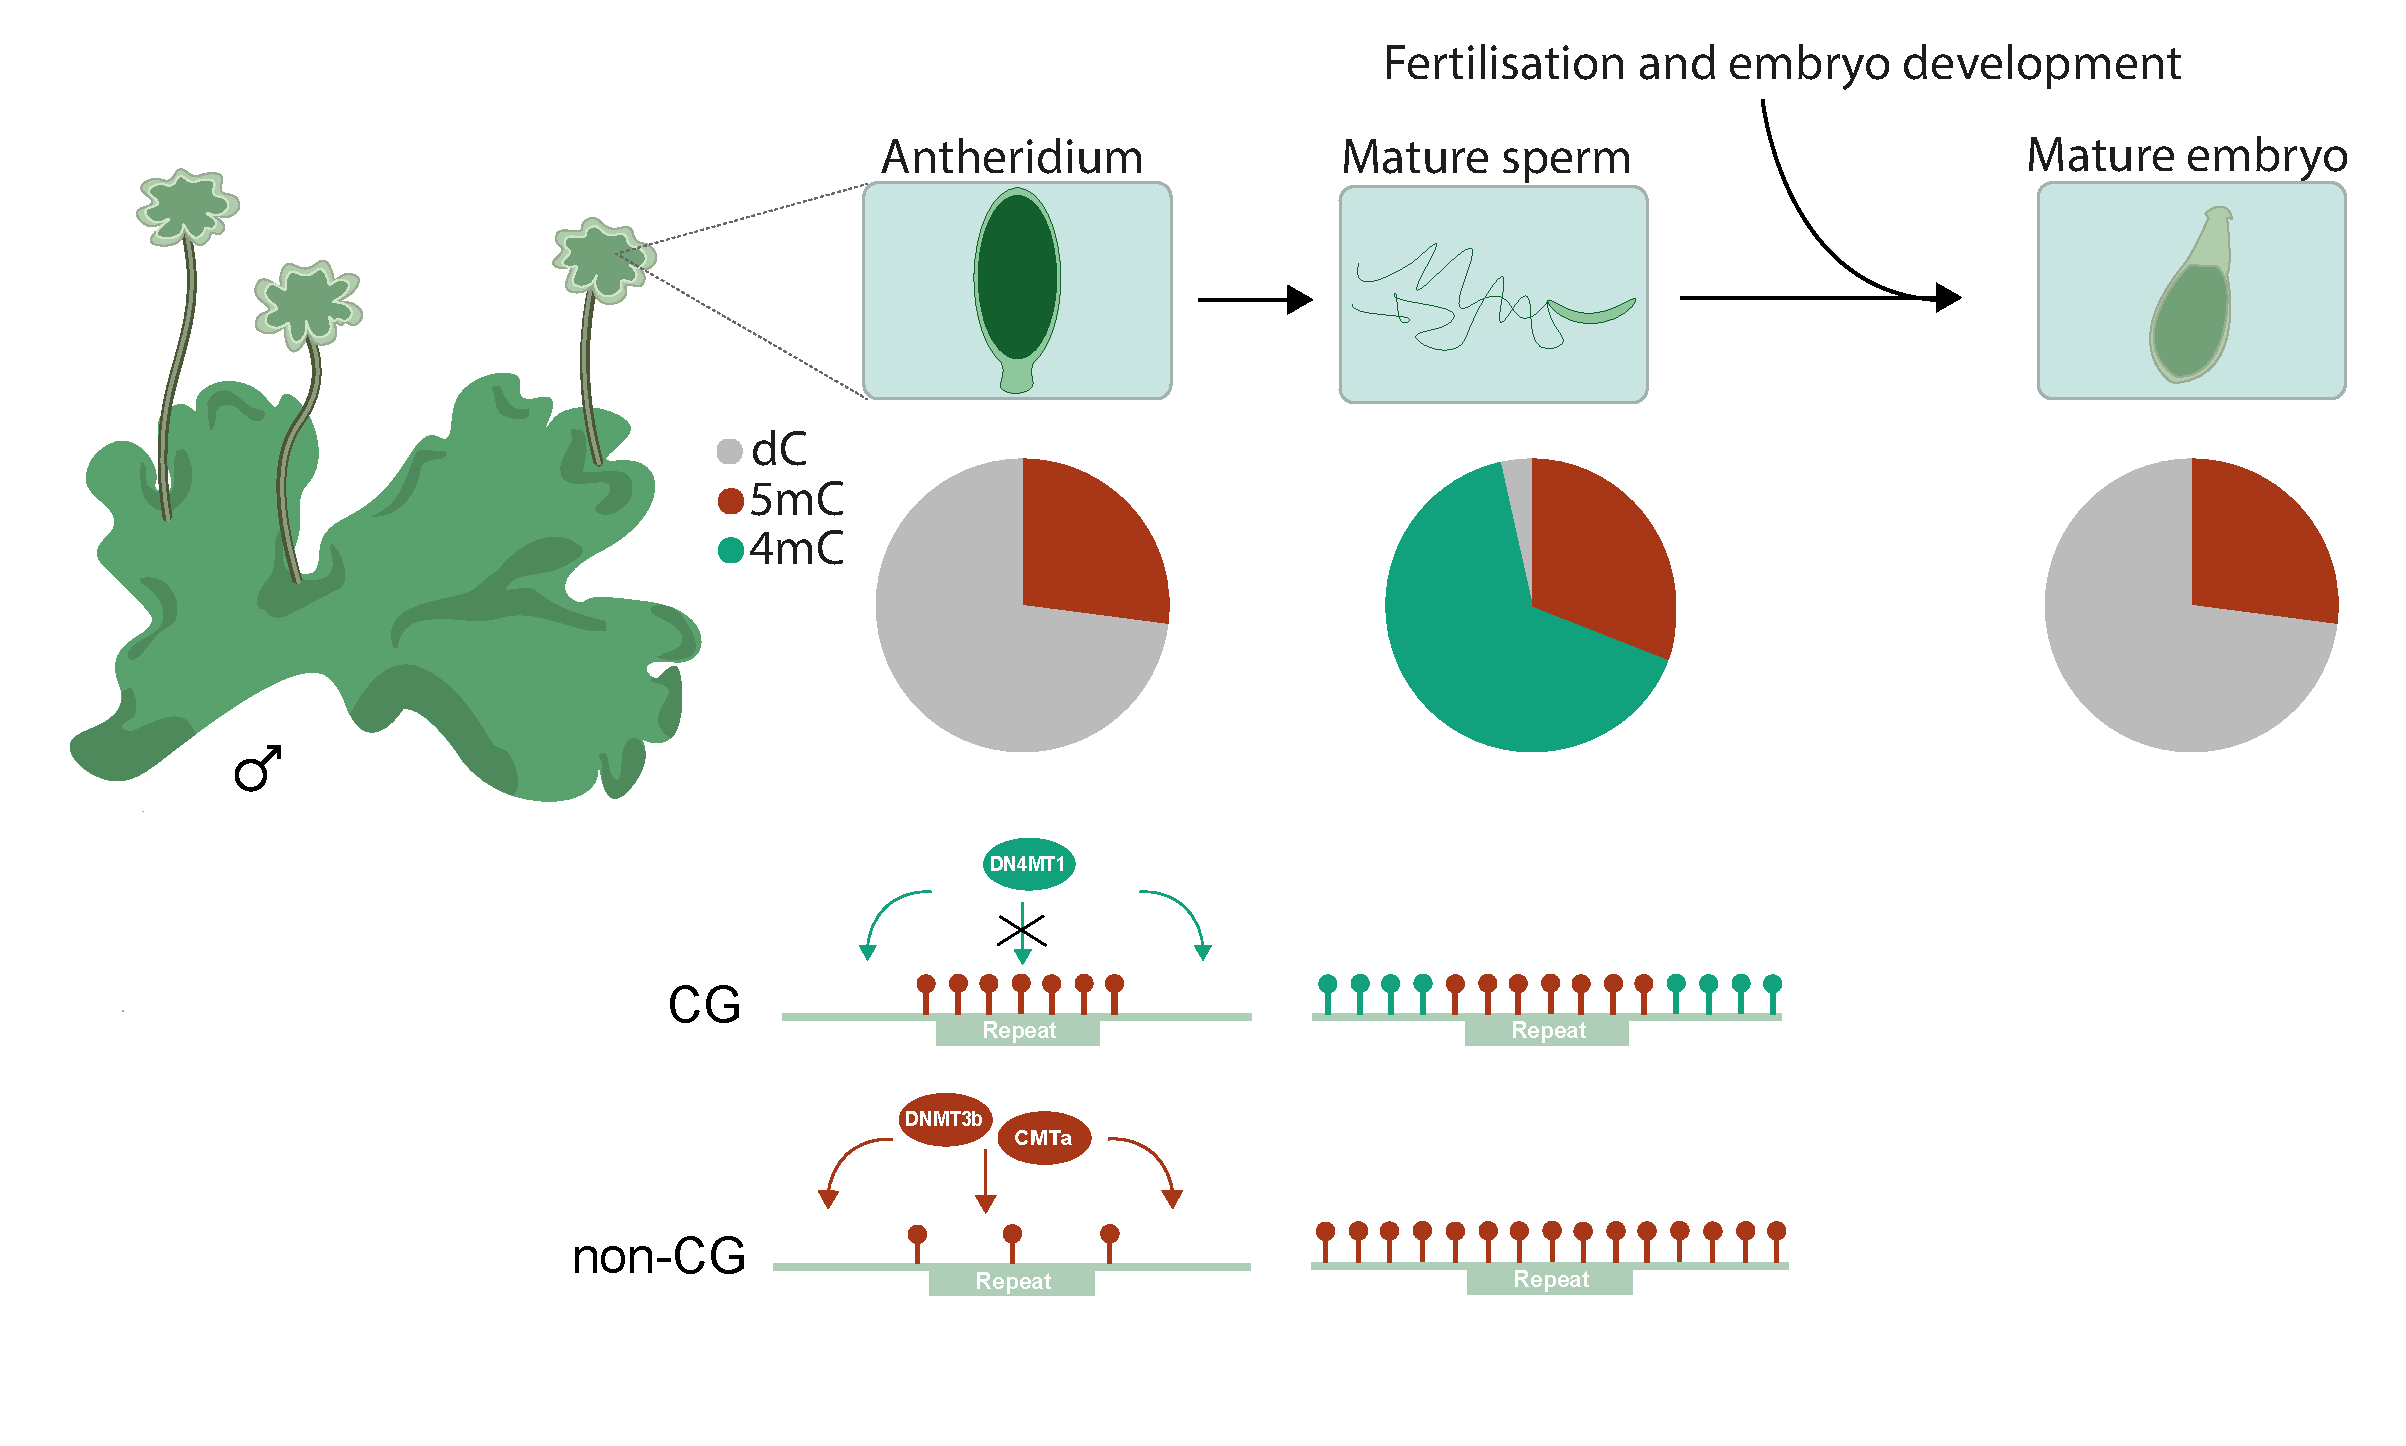
\includegraphics[width=1\textwidth]{Chapter3/Figs/Intro/Graphical_abstract.pdf}
\caption{}
\label{fig:Mp_graphical_abstract}
\captionsetup{font=small}
    \caption*{}
\end{figure}


Data from mature embryo reveals that this 4mC methylation is not present. Several hypotheses could explain why this happens. The most likely is that following fertilisation, paternal epigenetic marks are lost passively through cell division. Alternatively, the marks could be maintained through the first few cell divisions and then are actively or passively lost. We also know that the pronuclei take 3 days to fuse \citep{RN139}, so it is also possible that removing paternal epigenetic marks is required for zygote formation. 

Therefore, my project here will help complement the work that has already been done on 4mC methylation in Marchantia; please see our lab’s preprint for other details of this project \citep{RN189}. Namely, I have already managed to isolate and image embryos 12 days after fertilisation (DAF), and I plan to isolate and stage embryos that are as young as possible to make sure that we can detect 4mC signals if paternal epigenetic marks are maintained through zygote formation but are passively lost during cell division.

\subsection{Overview of DNA methylation in the germline of Marchantia polymorpha}

Recently, our group has shown that during Marchantia spermiogenesis extensive DNA methylation reprogramming occurs. As well as the deposition of 5-methylcytosine (5mC), there is an additional wave of DNA methylation reprogramming whereby N4-methylcytosine (4mC) – an epigenetic modification previously only found in prokaryotes – is deposited at the majority of CG cites across the genome \citep{RN189}.

However, this methylation is absent in the mature embryo (containing over 1000 cells). The exact point in time when 4mC methylation disappears post-fertilisation remains unknown, as does whether the paternal genome retains any 4mC marks during the early stages of zygotic development. The first division of the zygote in Marchantia takes place around 4 days post-fertilisation1 which suggests that 4mC may be required to be actively removed for pronuclear fusion to occur. This aligns with the observed phenotype where embryos fertilised by Mpdn4mt1 sperm develop more rapidly, though this phenotype needs to be confirmed during early embryonic development. Alternatively, 4mC methylation could be lost passively following fertilisation through dilution by cell division, or actively removed post-fertilisation for DNA replication or cell division to function normally. 4mC may also be crucial in the correct genome dosage/transcriptional activity during early embryonic development. 

In Arabidopsis, 5mC methylation is lost actively to maintain homeostasis of DNA methylation levels through several DNA glycosylases, including ROS1 \citep{RN168}. Therefore, the orthologs of ROS1 in Marchantia, MpROS1a and MpROS1x (located on the female sex chromosome) offer possible candidates for erasing paternal 4mC methylation as they are expressed in the sperm \citep{RN212} and mature eggs/embryos \citep{RN257} respectively.
DNA demethylases regulate DNA methylation levels in eukaryotes. Arabidopsis encodes four DNA demethylases, DEMETER (DME), REPRESSOR OF SILENCING 1 (ROS1), DEMETER-LIKE 2 (DML2), and DML3. While DME is involved in vegetative cell demethylation in pollen \citep{RN57} (as discussed in Chapter 2), it is also required for the allele-specific expression of maternally imprinted genes in the central cell and endrosperm \citep{RN235}. The rest of the DNA glycosylases seem to be functionally redundant and are involved in preventing the spread of transposon 5mC methylation to genic regions\citep{RN288}. \textit{Marchantia} has 2 orthologs of ROS1, one of which is found on the female chromosome ROS1X and is expressed specifically in the embryo \citep{RN169,RN257,RN189}. 

It has also recently been shown that other epigenetic marks, namely the heterochromatic histone modification H3K27me3 is deposited at the pronuclear stage exclusively on the paternal genome and causes the repression of the paternal genome persisting until the conclusion of embryogenesis \citep{RN160}. In contrast, in mammalian germlines, H3K27me3¬ mediated imprinting is limited to a few loci within the female gamete \citep{RN172}.

Hence, investigating the methylation profiles of early Marchantia embryos during the first zygotic divisions and examining the early developmental phenotype of Mpdn4mt1 mutants will complement our previous work, expanding our understanding of how paternal DNA methylation affects early embryonic development.

\begin{figure}[htbp!] 
\centering    
    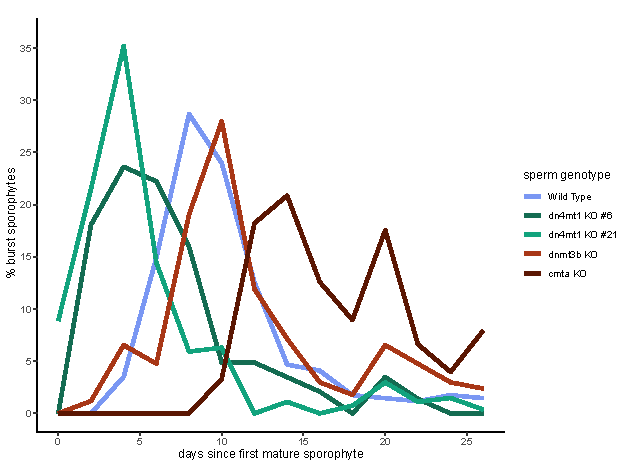
\includegraphics[width=1\textwidth]{Chapter3/Figs/Intro/burstpeak_nuclei_number.pdf}
\caption{\textbf{Embryos fertilised by \textit{dn4mt1} knockout sperm develop more rapidly than WT}}
\label{fig:burstpeak}
\captionsetup{font=small}
    \caption*{Total percentage of burst sporophytes every day since first mature sporophyte, fertilised with wild type sperm (blue), two independent lines of \textit{dn4mt1} knockout sperm (\#6 dark green, \#21 light green) or 5mC (\textit{cmta} (dark brown) or \textit{dnmt3B}) knockout sperm (light brown). }
\end{figure}

\clearpage

\section{Paternal 4mC is lost in the early embryo of \textit{Marchantia}}

To establish an effective method for staging early Marchantia embryos and identify the earliest feasible window for embryo extraction for AMD sequencing, several approaches were explored. Despite incorporating detergents, vacuum-assisted staining, and testing various stains (DAPI, Hoechst 33342, and ethidium bromide), live-cell staining of developing embryos within the archegonium remained inconsistent. This inconsistency likely arises from the embryo's position within a cavity (the venter) surrounded by somatic cells and cell walls (Figure \ref{fig:egg_embryo} rows one and two). Moreover, variations in environmental conditions during embryo development significantly impacted growth, as illustrated in Figure \ref{fig:embryo_diff} which shows the same genotype embryos 10 days post-fertilisation under different growth conditions. To ensure consistency and reproducibility, a controlled crossing method was adopted, wherein archegoniophores were exposed to sperm in a tube for an hour, ensuring synchronised fertilization and uniform embryo development. This approach is particularly suited for studying early embryo development, as embryos can be cultured under these conditions for up to two weeks\citep{RN139}. Under these conditions, the earliest developing embryos could be manually dissected was around 7-8 days after fertilisation (Figure \ref{fig:egg_embryo}).

\begin{figure}[htbp!] 
\centering    
    \includegraphics[width=1\textwidth]{Chapter3/Figs/Figure1_eggs_and_embryos.pdf}
\caption{\textbf{Live cell imaging of the developmental stages of \textit{M. polymorpha} embryos}}
\label{fig:egg_embryo}
\captionsetup{font=small}
    \caption*{Unstained egg cell (first row), DAPI stained egg cell (second row), and embryos 8 days (third row), and 10 days (fourth row) after fertilisation. Scale bar 10$\mu$m}
\end{figure}

As previously established, 4mC methylation is deposited in the CG context over gene bodies and outside of TEs during spermiogenesis by \textit{DN4MT1} (Figure \ref{fig:ends_analysis}A)\citep{RN189}. Although 5mC methylation across all sequence contexts over TEs increases during germline development, non-CG methylation is specifically deposited during spermiogenesis by \textit{MpCMTa} and \textit{MpDNMT3B} (Figure \ref{fig:ends_analysis}B,D,F)\citep{RN189}.  Additionally, this methylation pattern is deposited and maintained over gene bodies (excluding the transcription start site, TSS), with 4mC serving as the primary methylation mark at the TSS. 

As early embryos are difficult to harvest, first AMD-seq (sequencing specifically 4mC) and EM-seq (sequencing specifically 5mC) was tested on wild type sperm and compared to data previously collected from wild type sperm and \textit{dn4mt1} sperm(Figure \ref{fig:ends_analysis} WT sperm rep2 AMD-seq (light green) and dn4mt1 sperm AMD-seq(grey)). The expected methylation patterns over genes and TEs in the 4mC and 5mC contexts were confirmed by the sperm AMD-seq and EM-seq libraries (Figure \ref{fig:ends_analysis} wild type sperm rep2 AMD-seq(light green), wild type sperm EM-seq(dark brown).) 

\begin{figure}[htbp!] 
\centering    
    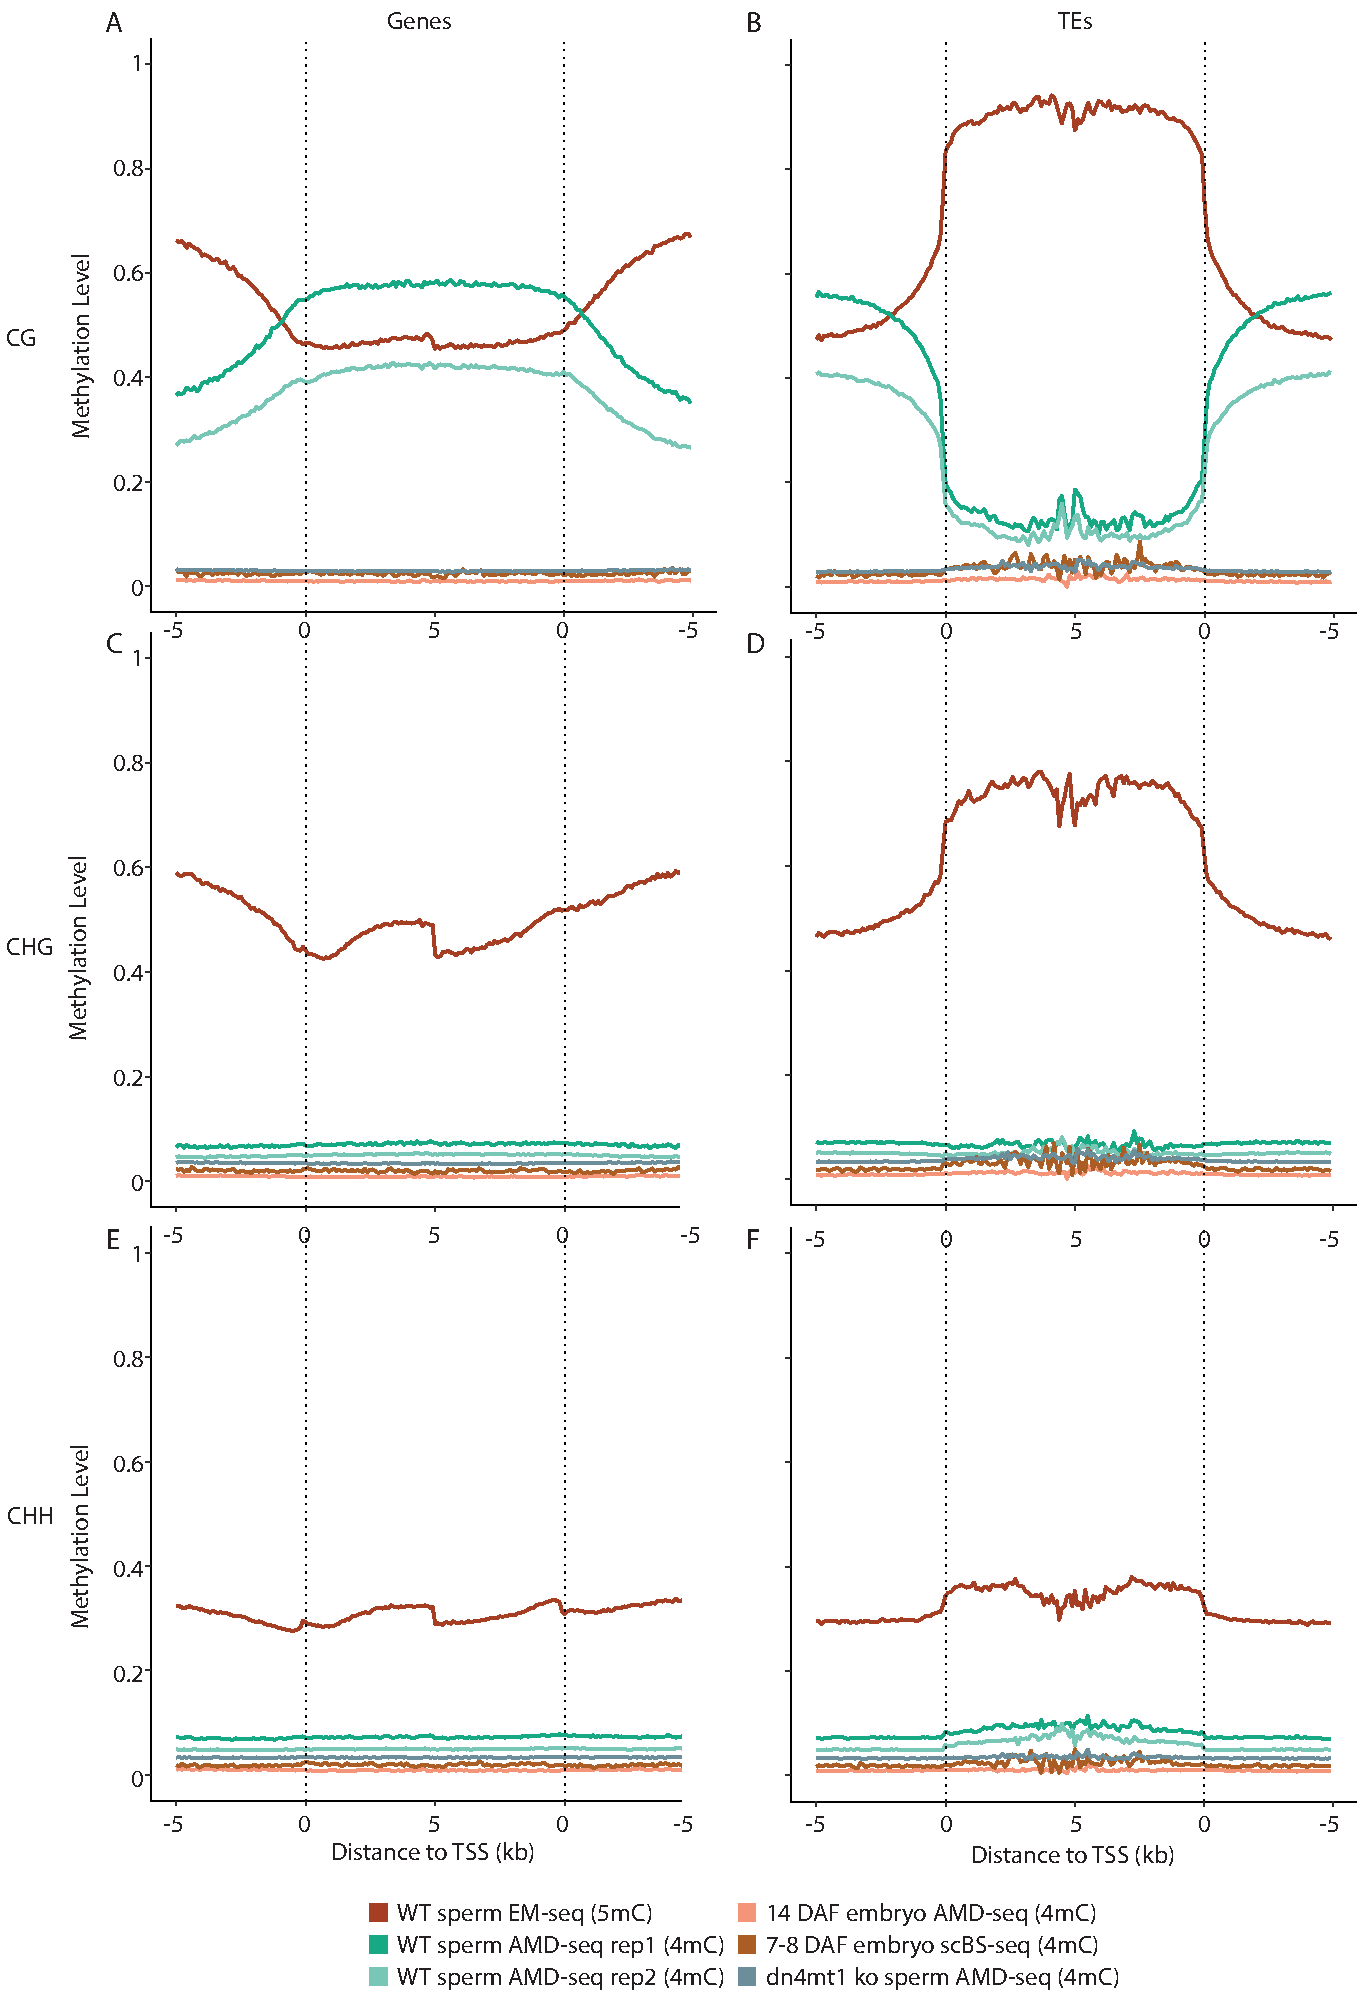
\includegraphics[width=1\textwidth]{Chapter3/Figs/Figure2_ends_analysis.pdf}
\caption{\textbf{4mC methylation occurs in the CG context and is enriched in genic regions and outside of TEs, while 5mC methylation is largerly confined to TEs}}
\label{fig:ends_analysis}
\captionsetup{font=small}
    \caption*{Panel showing 4mC and 5mC methylation across TEs (A) and Genes (B) in CG (first row), CHG (second row) and CHH (third row) sequence contexts in wild type sperm \textit{dn4mt1 sperm}, the embryo 7-8 and 14 days after fertilisation.}
\end{figure}

Secondly, pre-meiotic embryos were dissected and sequenced using AMD-seq to establish a baseline for comparing early embryonic methylation patterns (Figure \ref{fig:ends_analysis}, 14 DAF embryos (orange)). The results confirmed the absence of 4mC methylation over genes or outside TEs (Table \ref{tab:methylation_levels}). Subsequently, 300 embryos at 7–8 DAF were collected, with 200 used for AMD sequencing library construction and the remaining 100 embryos used for bisulfite sequencing libraries, pre-treated with APOBEC3A for an alternative 4mC sequencing method. Although AMD-seq is theoretically capable of handling low DNA input down to picogram levels\citep{idtdna_methylseq_kit}, this was not tested prior to sequencing the early embryos.The bisulfite sequencing protocol, on the other hand, was developed for low-input or single-cell sequencing and this has been robustly tested in our lab. Due to conversion issues, the AMD-seq library was not usable in this study. 

\begin{figure}[htbp!] 
\centering    
    \includegraphics[width=1\textwidth]{Chapter3/Figs/Figure3_H3K27me3.pdf}
\caption{\textbf{H3K27me3 levels are elevated in the paternal genome and correlate with the presence of 5mC over genes}}
\label{fig:h3k27me3}
\captionsetup{font=small}
    \caption*{Heatmaps showing the relative H3K27me3 levels in Marchantia embryos over the genes and TEs in the paternal and maternal genomes.}
\end{figure}

At a surface level, the early embryo AMD-seq data indicated marginally higher 4mC methylation across genes compared to the mature AMD sequencing library (Figure \ref{tab:methylation_levels}). However, this increase fell within the error range of the experimental limitations (Table \ref{tab:methylation_levels}, "CHG and CHH levels of 4mC"). Moreover, the low levels of residual 4mC methylation did not display the expected distribution over genes and TEs, with no relative increase outside TEs or over genes. This suggests that the removal of paternal 4mC methylation may be essential for embryo development. However, starting with a methylation level of around 20\% in the zygote (based on the sperm AMD-seq levels), passive loss of 4mC by the 16–32 cell stage (7–8 days after fertilisation in our conditions) would result in very low residual 4mC methylation levels (Table \ref{tab:methylation_levels}). 

It has been previously demonstrated that during embryonic development the paternal genome is transcriptionally silenced and is marked with the repressive chromatin mark H3K27me3 mediated by maternally expressed Polycomb Repressive Complex 2 (PRC2) in the male pronucleus before the first zygotic division, approximately 3 days after fertilisation \citep{RN160}. This suggests the existence of a mechanism for paternal genome recognition, with blanket 4mC methylation being a potential candidate. To this end, visualizing H3K27me3 data across genes and TEs from this study confirms a paternal bias in the deposition of H3K27me3. However, the pattern of H3K27me3 occupancy around gene and transposon transcription start sites does not align with the distribution of 4mC.

\begin{table}[htbp!]
\centering
\captionsetup{font=small}
\begin{tabular}{|p{5cm}|c|c|c||c|c|c|}
\hline
\multirow{2}{*}{\makecell{Methylation context}} & \multicolumn{3}{c||}{Overall} & \multicolumn{3}{c|}{Genes} \\
\cline{2-7}
 & CG & CHG & CHH & CG & CHG & CHH \\
\hline
WT sperm AMD seq rep1 & 0.467 & 0.071 & 0.075 & 0.559 & 0.071 & 0.072 \\
WT sperm AMD seq rep2 & 0.341 & 0.050 & 0.051 & 0.404 & 0.051 & 0.049 \\
dn4mt1 ko sperm & 0.031 & 0.035 & 0.033 & 0.029 & 0.034 & 0.033 \\
14 DAF embryo & 0.011 & 0.009 & 0.009 & 0.009 & 0.008 & 0.008 \\
7-8 DAF embryo & 0.027 & 0.021 & 0.019 & 0.025 & 0.020 & 0.020 \\
\hline
\multicolumn{7}{|l|}{Theoretical methylation levels} \\
\hline
Zygote & 0.202 & 0.030 & 0.031 & 0.241 & 0.030 & 0.030 \\
16 cell embryo  & 0.013 & 0.016 & 0.015 & 0.015 & 0.015 & 0.015 \\
32 cell embryo & 0.006 & 0.007 & 0.007 & 0.008 & 0.007 & 0.007 \\
\hline
\end{tabular}
\caption{\textbf{Methylation levels across WT sperm, \textit{dn4mt1} sperm and the early embryo}}
\label{tab:methylation_levels}
\end{table}


\section{\textit{De novo} methylation is deposited in genic regions specifically in the sporophyte of \textit{Marchantia}, targeted for methylation 24nt sRNAs through mismatches}

As described previously, \textit{de novo} metylation of genes in \textit{Arabidopsis} male meiocytes is mediated by 24nt sRNAs produced by HyperTE loci in the tapetum, the biogenesis of which is iven by CLSY3 chromatin remodeller. Gene body methylation also exists specifically in the embryo and sporophyte of \textit{Marchantia} (Figure \ref{fig:SLM_examples}, data from Dr. James Walker). Sporophytic non-CG DMRs were determined as described before\citep{jimmythesis} and filtered to yield 221 metylated genic loci (MetGenes).

\begin{figure}[htbp!] 
\centering    
    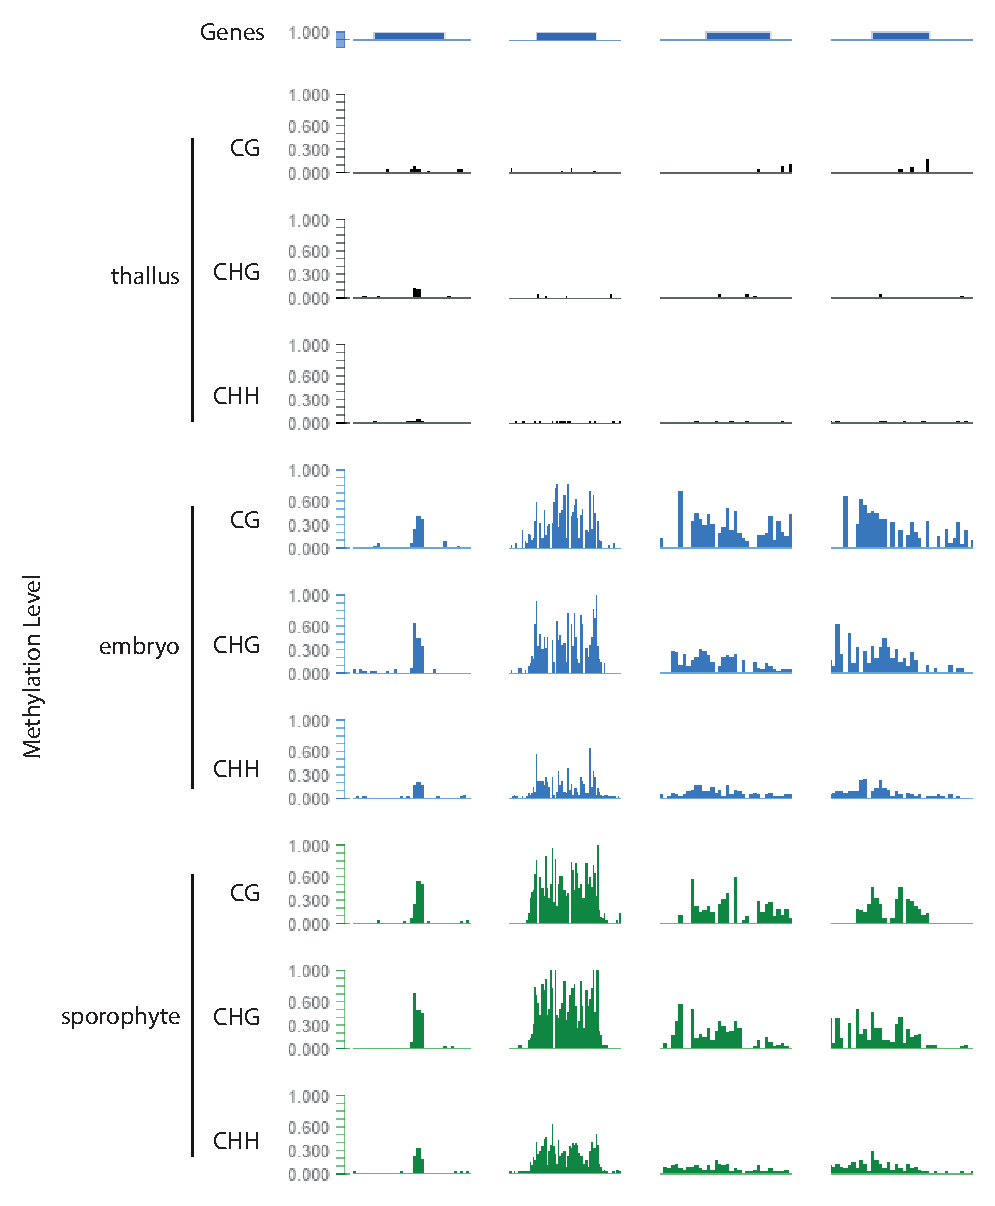
\includegraphics[width=1\textwidth]{Chapter3/Figs/Figure4_SLM_examples.pdf}
\caption{\textbf{Sporophyte specific methylation exists in the embryos of \textit{Marchantia}}}
\label{fig:SLM_examples}
\captionsetup{font=small}
    \caption*{}
\end{figure}

With access to sRNA sequencing libraries from thallus, embryo, and sporophyte, the next step was to determine whether MetGenes could be targeted for methylation through mismatch targeting. To investigate this, the sRNA libraries were mapped to the reference genome allowing for 0 and 3 mismatches. The sRNAs from the 3 mismatch dataset were then remapped onto the 0 mismatch dataset to identify identical sRNA sequences capable of targeting both TEs and genes with up to 3 mismatches. Reads overlapping MetGenes with 3 mismatches and TEs with 0 mismatches were then extracted. The resulting TE-MetGene pairs are visualised in Figure \ref{fig:SLM_targeting}A. It must be noted that one limitation of this method is the challenge of obtaining a comprehensive TE annotation for the gene model used in the study, as not all MetGenes could be paired with annotated TEs.

Indeed when aligning the sequence of a source TE to its corresponding MetGene, an almost perfectly matching \~160bp sequence was found (Figure \ref{fig:SLM_targeting}B). Notably, this alignment corresponds to the exact location where sporophyte-specific methylation is deposited within the MetGene (Figure \ref{fig:TE_SLM_pairs}).

\begin{figure}[htbp!] 
\centering    
    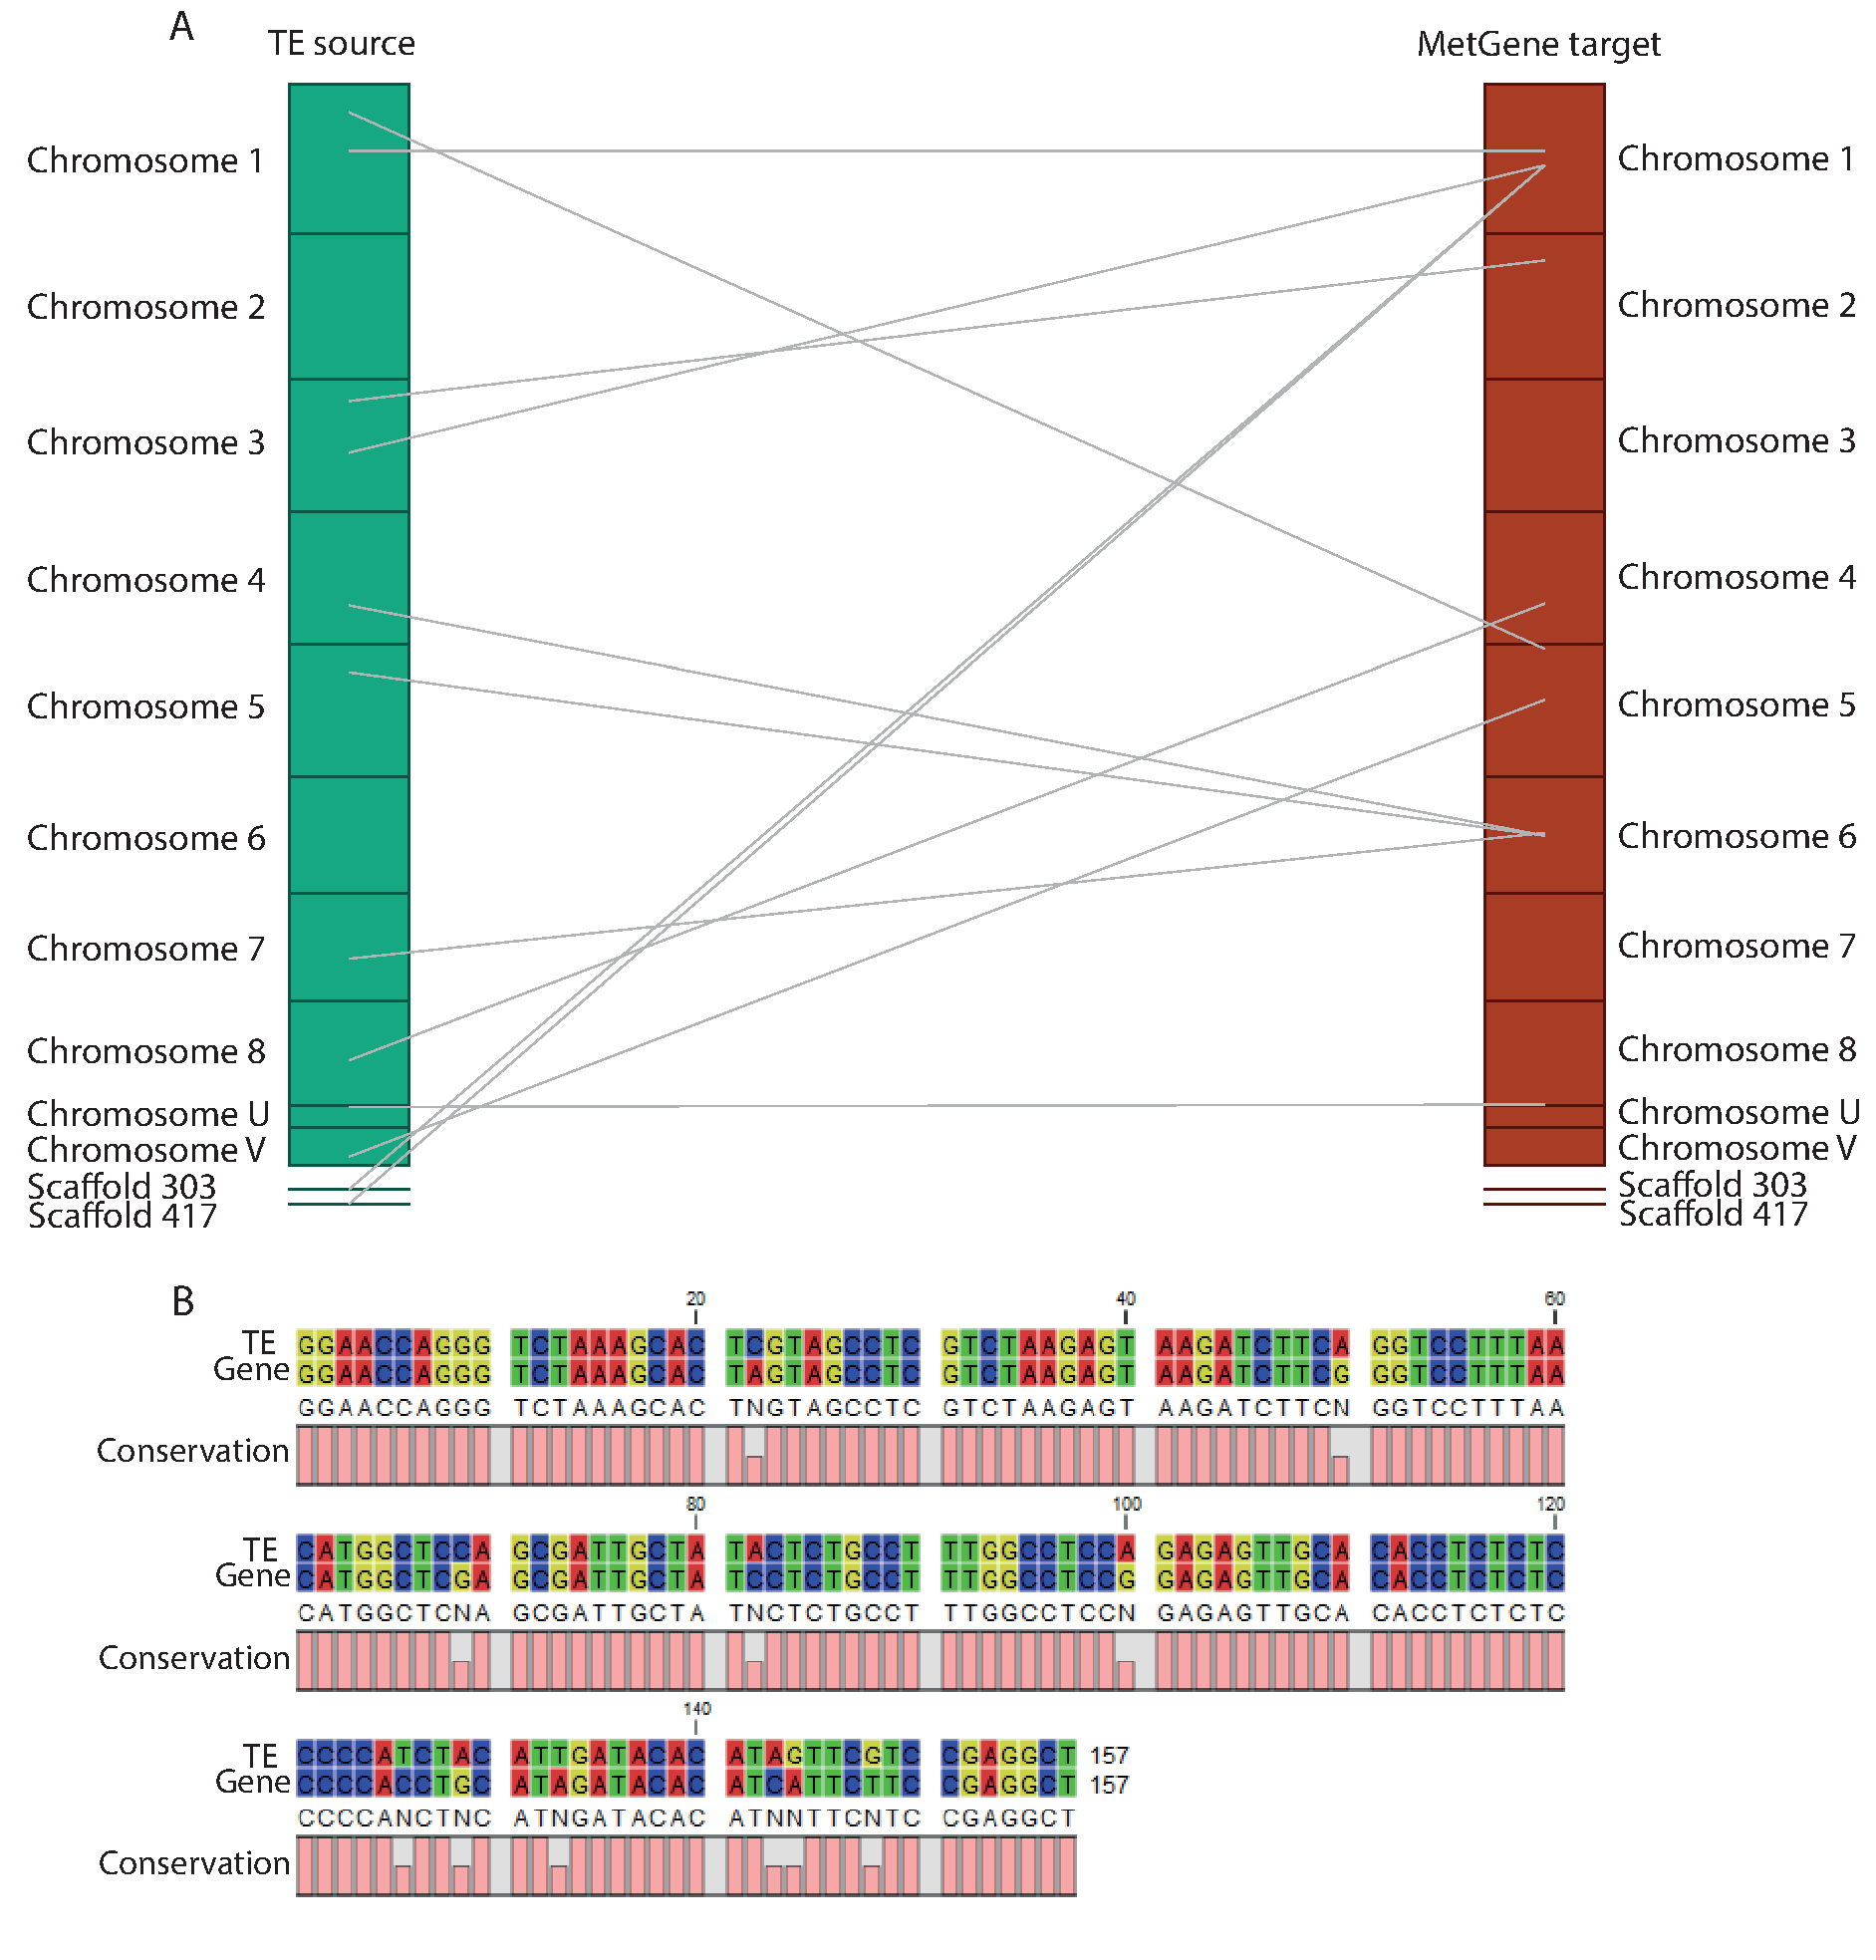
\includegraphics[width=1\textwidth]{Chapter3/Figs/Figure5_SLM_source_target.pdf}
\caption{\textbf{TE loci produce 24nt sRNA that target genic loci for methylation with mismatch targeting}}
\label{fig:SLM_targeting}
\captionsetup{font=small}
    \caption*{Locations of TE source loci (left, green) connected to genic target loci (right, brown)}
\end{figure}

\begin{figure}[htbp!] 
\centering    
    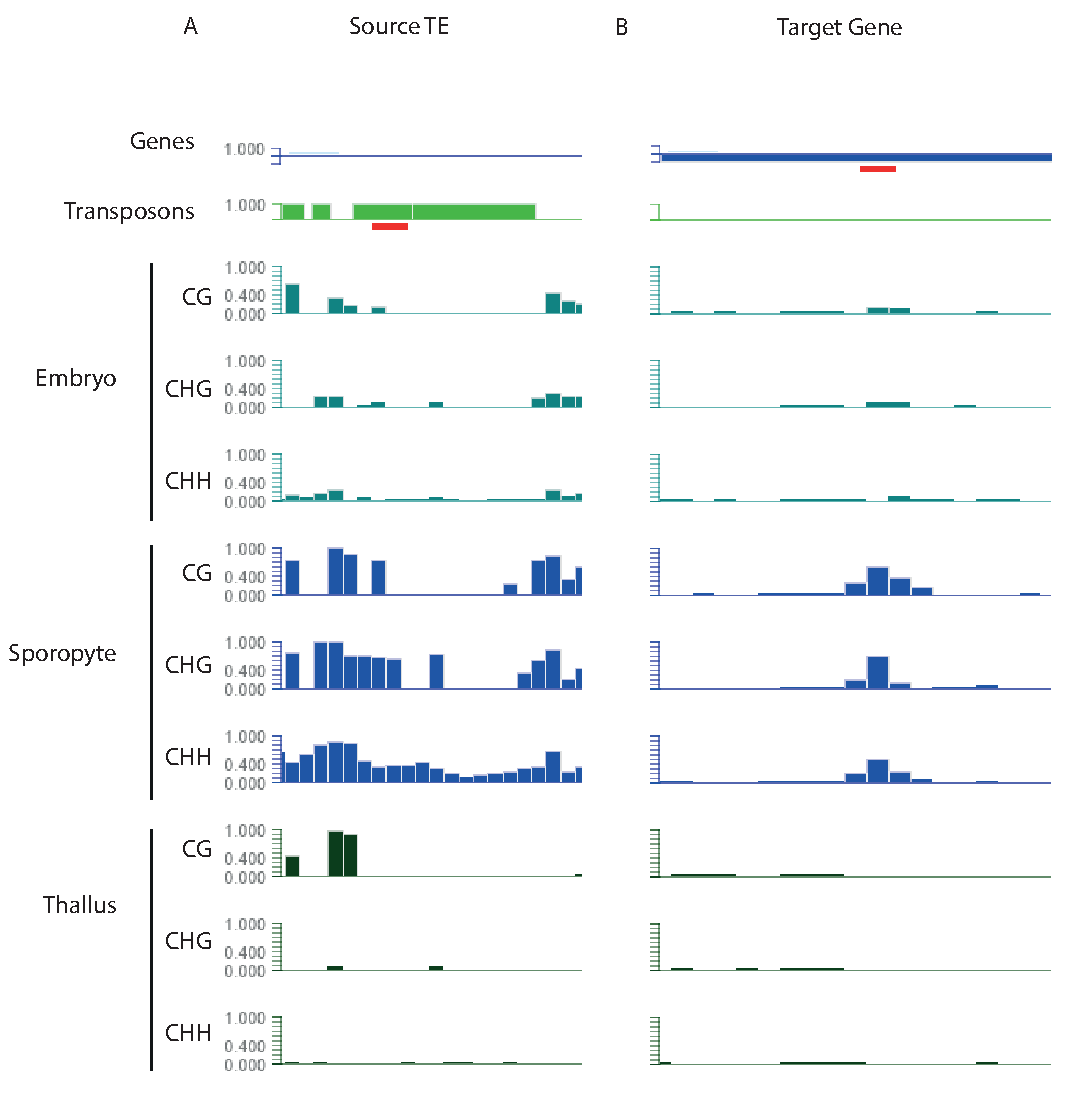
\includegraphics[width=1\textwidth]{Chapter3/Figs/Figure6_pairs_examples.pdf}
\caption{\textbf{Example of a TE  source and SLM target that gain methylation in the sporophyte}}
\label{fig:TE_SLM_pairs}
\captionsetup{font=small}
    \caption*{Methylation levels in (A) TE source and (B) SLM target pair in CG, CHG and CHH sequence contexts in embryo, sporophyte and thallus. Overlapping sequence highlighted in red.}
\end{figure}

\section{Investigating the parental bias of sRNA production in \textit{Marchantia} embryos, sporophyte and thallus}

In the developing embryo, the paternal genome is deposited with H3K27me3, resulting in tight heterochromatic foci and transcriptional silencing \citep{RN160}. This raises the question of whether sRNA production in the embryo and sporophyte is biased toward the maternal genome.To explore this, single nucleotide polymorphisms (SNPs) between Tak-1 (male) and Tak-2 (female) were analysed to calculate a SNP ratio. sRNA sequencing libraries utilised from the thallus, archegoniophore, and antheridiophore \citep{RN265} in addition to the libraries previously mentioned.

The sRNA sequencing libraries were mapped to the reference genome with both no mismatches, and allowing one mismatch. Reads with mismatches at SNP positions were retained, as well as perfect matching sRNAs at SNP positions. A SNP ratio was calculated between the alternative and reference alleles for further analysis. Although several thousand SNP regions were initially covered, only those with at least 5 reads were retained to ensure robust results, which substantially reduced the number of SNP locations. 

Reads from archegoniophores displayed a SNP ratio near 1, as expected (Figure \ref{fig:sRNA_SNPs}A,B archegoniophore). Interestingly, in the early embryo, the data suggest a paternal bias in sRNA production, which shifts to a maternal bias in the sporophyte (Figure \ref{fig:sRNA_sizes}A,B embryo and sporophyte). As expected, the SNP ratio distribution in the embryo and sporophyte was less bimodal than in other tissues, indicating concurrent sRNA production from both genomes at multiple loci in the diploid phase. The thallus data seemed unreliable, with a surprising maternal bias despite originating from Tak-1 males \citep{RN265}.

\begin{figure}[htbp!] 
\centering    
    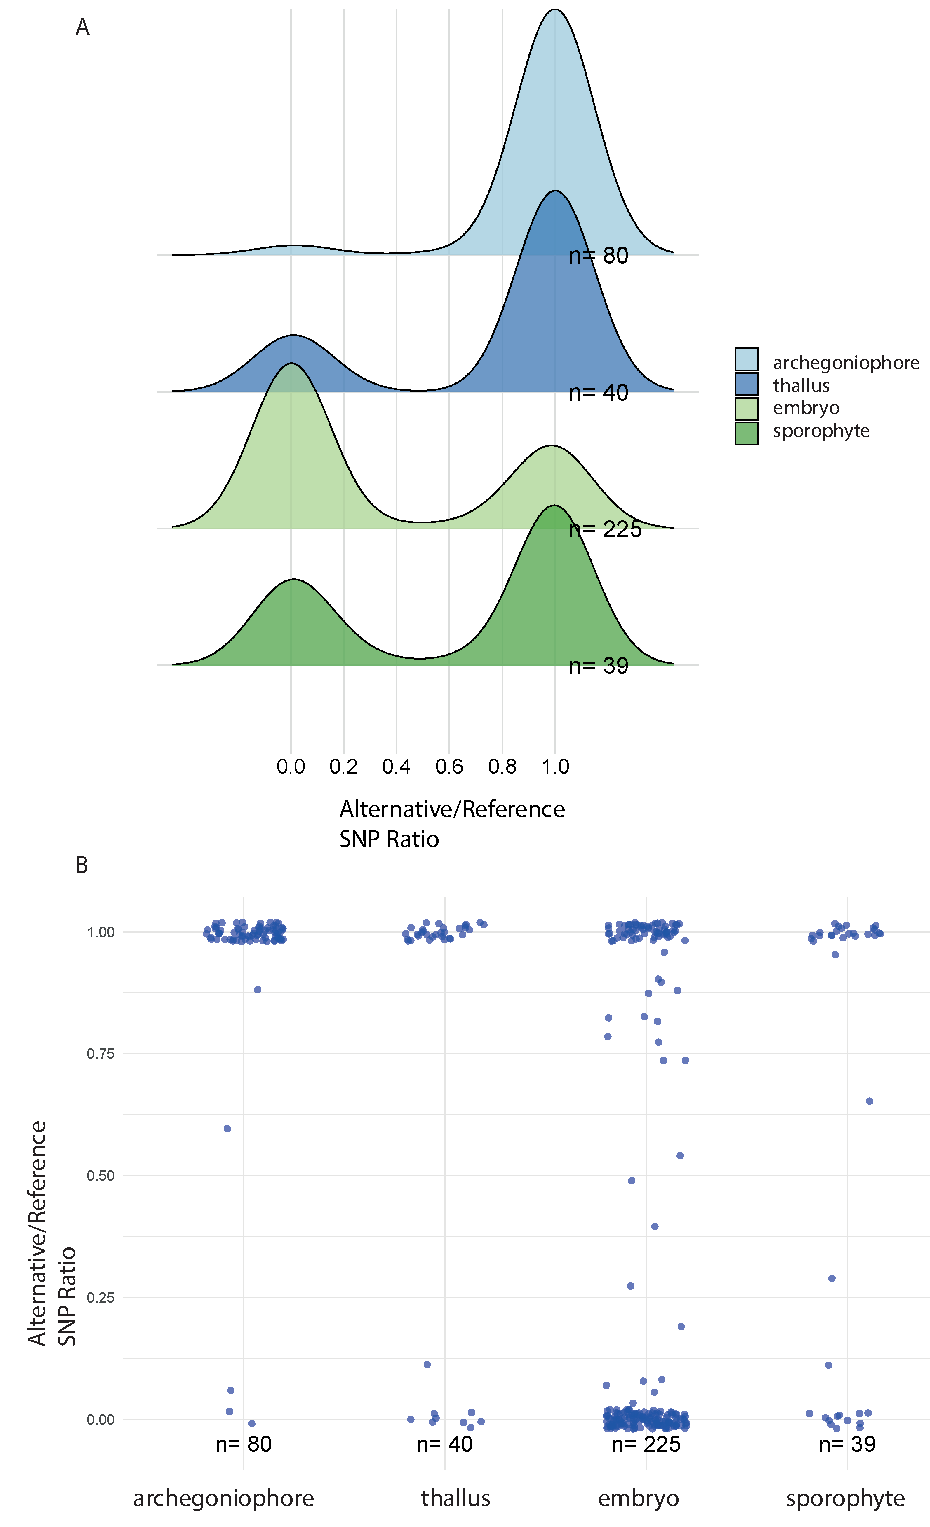
\includegraphics[width=1\textwidth]{Chapter3/Figs/Figure_sRNA_SNPs.pdf}
\caption{\textbf{}}
\label{fig:sRNA_SNPs}
\captionsetup{font=small}
    \caption*{}
\end{figure}

\clearpage

\section{Developing an effective method for visualising early embryonic development in \textit{Marchantia}}

The next objective was to determine whether the observed phenotype — where embryos fertilised with 4mC methylation mutants reach maturity earlier than wild type (Figure \ref{fig:burstpeak}) — was due to accelerated pronuclear fusion in the zygote, potentially caused by the absence of paternal 4mC. This led to the hypothesis that paternal 4mC may need to be actively removed before pronuclear fusion can occur.

As described earlier, staining live \textit{Marchantia} embryos proved challenging. A variety of fixing and staining methods were also trialled, including DAPI, Hoechst 33342 and ethidium bromide as staining dyes (the latter was used due to its small molecule size, which was expected to penetrate the fixed embryo), as well as different triton and paraformaldehyde concentrations and fixation times. Additionally, an egg cell reporter line was also tested (ECpro:MpSUN-GFP \citep{RN139}) showing strong expression; this faded after the first zygotic division, making it insufficient for visualizing early embryonic development (Figure \ref{fig:MpSUN}). 

Next, cell wall digestion enzymes such as cellulase and pectinase were trialed to improve dye penetration. While these enzymes increased dye uptake, they also compromised cell ultrastructure, hindering proper imaging of early embryonic development and cellular ultrastructure (Figure \ref{fig:enzyme_tests}). As a result, four constructs were designed to create constitutively expressing nuclear reporter lines. These constructs were driven by either the constitutive 35S promoter or the native EF$\alpha$ promoter, fused with citrine or tdTomato, and tagged with a nuclear localisation signal (NLS) (Figures \ref{fig:35S_citrine_map}, \ref{fig:35S_tdTomato_map}, \ref{fig:EFalpha_citrine_map}, \ref{fig:EFalpha_tdTomato_map}). 

\begin{figure}[htbp!] 
\centering    
    \includegraphics[width=1\textwidth]{Chapter3/Figs/Figure7_Reporter_line_gemmae_screening.pdf}
\caption{\textbf{Gemmae screening of constitutively expressed nuclear reporter lines}}
\label{fig:gemma:screen}
\captionsetup{font=small}
    \caption*{Nuclear signal of tdTomato or citrine (second column, red or yellow respectively, white arrows) in gemmae, driven by either 35S constitutive promoter (first row) native constitutive promoter EF$\alpha$ (second and third rows). Scale bar 10$\mu$m.}
\end{figure}

The constructs were initially transformed into Tak-1 thalli and selected in gemmae to avoid chimeric expression, resulting in the recovery of several independent lines from three of the four constructs (Figure \ref{fig:gemma:screen}).The constructs were then also transformed into sporelings from WTxWT, WTx\textit{dn4mt1} \#6 knockout and WTx\textit{dn4mt1} \#21 knockout crosses. Transformants were successfully recovered and screened for fluorescence expression in gemmae and antheridia (Figure \ref{fig:antheridia_screen}). Interestingly, while citrine reporter lines showed strong expression in gemmae, the strongest and most consistent expression was observed in transformants with the 35S::tdTomato-NLS and EF$\alpha$::tdTomato-NLS constructs. These lines were selected for crosses with wild-type female archegonia.

\begin{figure}[htbp!] 
\centering    
    \includegraphics[width=1\textwidth]{Chapter3/Figs/Figure8_Reporter_line_antheridia.pdf}
\caption{\textbf{The tdTomato based nuclear reporter lines are expressed in the antheridia}}
\label{fig:antheridia_screen}
\captionsetup{font=small}
    \caption*{Nuclear signal of tdTomato or citrine (second column, red or green respectively) in the antheridiophore, driven by either 35S constitutive promoter (first row) native constitutive promoter EF$\alpha$ (second and third rows). Scale bar 10$\mu$m.}
\end{figure}

Unfortunately, despite strong expression in the antheridia, no nuclear reporter expression was detected in the developing zygote or embryo.This may be attributed to the previously mentioned shutdown of the paternal genome (Figure \ref{fig:malevsfemale}, first and second rows).  In response to this, wild-type female plants were recovered from the WTxWT 35S::tdTomato-NLS and  EF$\alpha$::tdTomato-NLS sporeling crosses (Figure \ref{fig:malevsfemale}, rows 3 and 4) with strong expression their respective nuclear reporter lines. To improve clarity and fluorescence signal, a different clearing and staining method was employed, namely iTOMEI \citep{RN279}. In this protocol, the fixing component caprylyl sulfobetaine is able to clear chlorophyll without significantly quenching GFP (or other) fluorophores. After testing several environmental conditions, the best images were collected from 1\% FA fixation in PBS (pH 7.4) buffer for an hour, followed by clearing with caprylyl sulfobetaine for 24 hours (please see Materials and Methods for further details).


\begin{figure}[htbp!] 
\centering    
    \includegraphics[width=1\textwidth]{Chapter3/Figs/Figure9_reporter_line_malevsfemale.pdf}
\caption{\textbf{Tak1 male nuclear reporter lines crossed to Tak2 females have no nuclear expression in the embryo}}
\label{fig:malevsfemale}
\captionsetup{font=small}
    \caption*{Nuclear signal of tdTomato (second column, red, white arrows) in embryos crossing EF$\alpha$::tdTomato-NLS Tak1 male to WT Tak2 female, 3 days (first row) and 16 days (second row) after fertilisation. Expression of EF$\alpha$::tdTomato-NLS (third row) and  35S::tdTomato-NLS (fourth row) in WT female thallus. Scale bar 10$\mu$m.}
\end{figure}

\section{Embryos crossed with 4mC metylation mutant sperm develop more rapidly than wild type during the first 7 days post-fertilisation}

Once mature archegoniophore-producing female plants were available from the selected 35S::tdTomato-NLS and EF$\alpha$::tdTomato-NLS lines, they were crossed with WT, \textit{dn4mt1} \#6 and \textit{dn4mt1} \#21 sperm. As before, the sperm was co-cultured with the archegoniophores for an hour, after which the developing embryos were dissected carefully, fixed and cleared daily, 1 to 7 days post-fertilisation. Due to the use of immature archegoniophores, embryos at 3 DAF were unfortunately unsuitable for imaging. In total, 338 embryos were imaged during the 7 days post-fertilisation and the developmental stages manually determined. 

\begin{figure}[htbp!] 
\centering    
    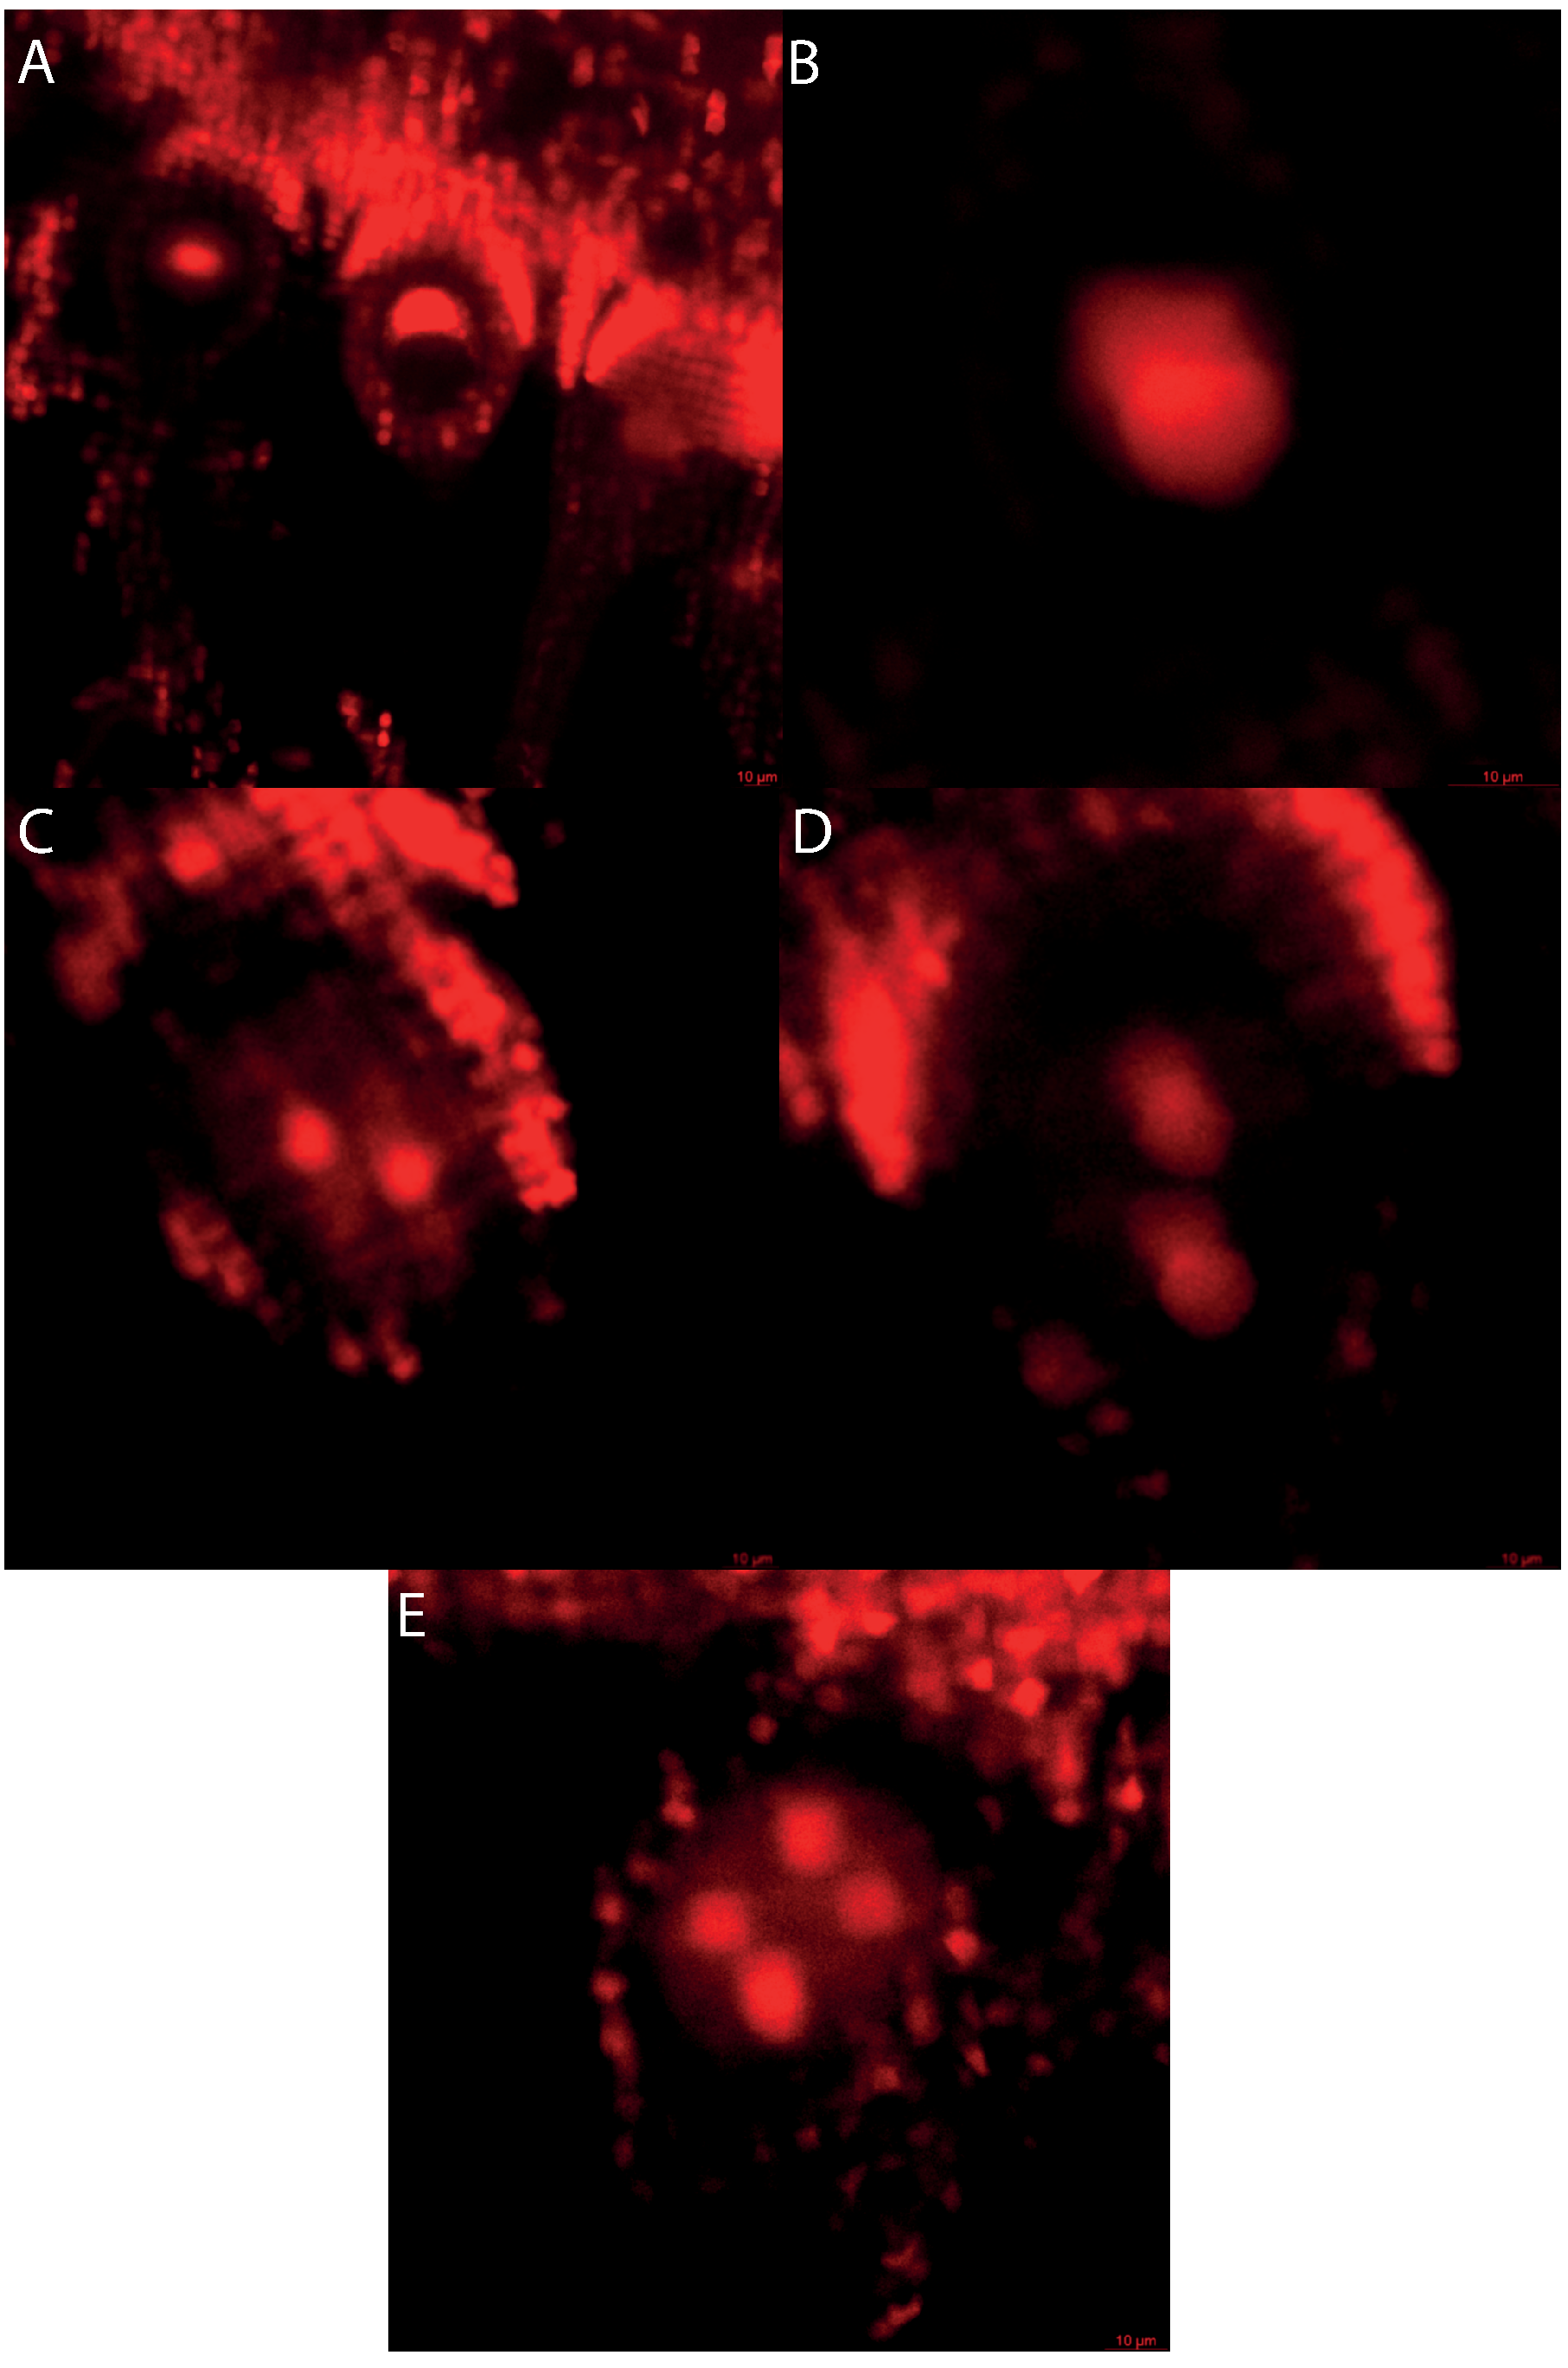
\includegraphics[width=1\textwidth]{Chapter3/Figs/Figure10_Developmental_stages.pdf}
\caption{\textbf{Developmental stages of the early embryo (Tak1 male x EF$\alpha$::tdTomato-NLS WT female)}}
\label{fig:dev_stages}
\captionsetup{font=small}
    \caption*{(A) Zygote (B) Zygote dividing (C) Two-cell stage (D) Two-cell embryo dividing (E) Four-cell stage. Scale bar 10$\mu$m.}
\end{figure}

The developing embryo initially elongates through a transverse division, perpendicular to the archegonial axis, followed by a second vertical division to form four cells. The third division occurs at right angles to the previous ones, creating an octant of equal cells \citep{RN143,RN144}. Subsequent cell divisions progressively alter the embryo's initially circular shape. To further assess early cellular development, in addition to counting the nuclei, the transverse diameter of the embryonic venter cavity was measured. Interestingly, the mean transverse diameter of the embryos remained consistent and increased at a similar rate across all lines all until day 6, and between WT and \textit{dn4mt1} k.o. \#6 between days 6 and 7 \ref{fig:transverse_diameter}.

During the first two zygotic divisions, cells were frequently observed with multiple nuclei that had not yet undergone cytokinesis (Figure \ref{fig:dev_stages}B and D).  To facilitate tracking of cell development, these different stages were classified into distinct developmental phases:1. 1 nucleus 2. 2 nuclei, 1 cell, 3. 2 nuclei, 2 cells 4. 4 nuclei, 2 cells, 5. 4 nuclei, 4 cells, 6. 8 nuclei, 4 cells, 7. 8 nuclei, 8 cells, 8. 9-16 nuclei, 9. 16-25 nuclei, 10. 26-35 nuclei, 11. 36-45 nuclei, 12. 46 - 55 nuclei, 13. more than 55 nuclei.

Between days 1 and 5 post-fertilisation, embryos fertilised by either of the independent \textit{dn4mt1} knockout lines appeared to initiate division earlier than those fertilised by wild-type sperm. For example, by day 2, nearly all imaged cells in the \textit{dn4mt1} knockout lines had 2 nuclei, compared to fewer than a quarter in the wild type (Figure \ref{fig:nucleus_number}B,C).  

This trend persisted through day 4, where approximately a quarter of cells in the \textit{dn4mt1} knockout line \#6 had reached stage 4, while none of the wild-type cells had progressed that far. By day 5, the proportion of cells in various developmental stages became more synchronized across the genotypes. However, after day 5, embryos from the \textit{dn4mt1} knockout line \#21 continued to develop more rapidly than the wild type, the most advance embryos reaching stage 13 by day 6 compared to stage 10 in wild-type (Figure \ref{fig:nucleus_number}B,C). 

In contrast, the difference between the wild type and the \textit{dn4mt1} knockout line \#6 was less pronounced, with some embryos from a \textit{dn4mt1} \#6 background reaching stage 12 by day 7, while the most developed wild type embryos were slightly behind, in stage 11. It is also noteworthy that embryos from a  \textit{dn4mt1} \#6 knockout background displayed a proportion of cells arrested in stage 1 or 2, even at day 6 and day 7 (\ref{fig:nucleus_number}B,C).


\begin{figure}[htbp!] 
\centering    
    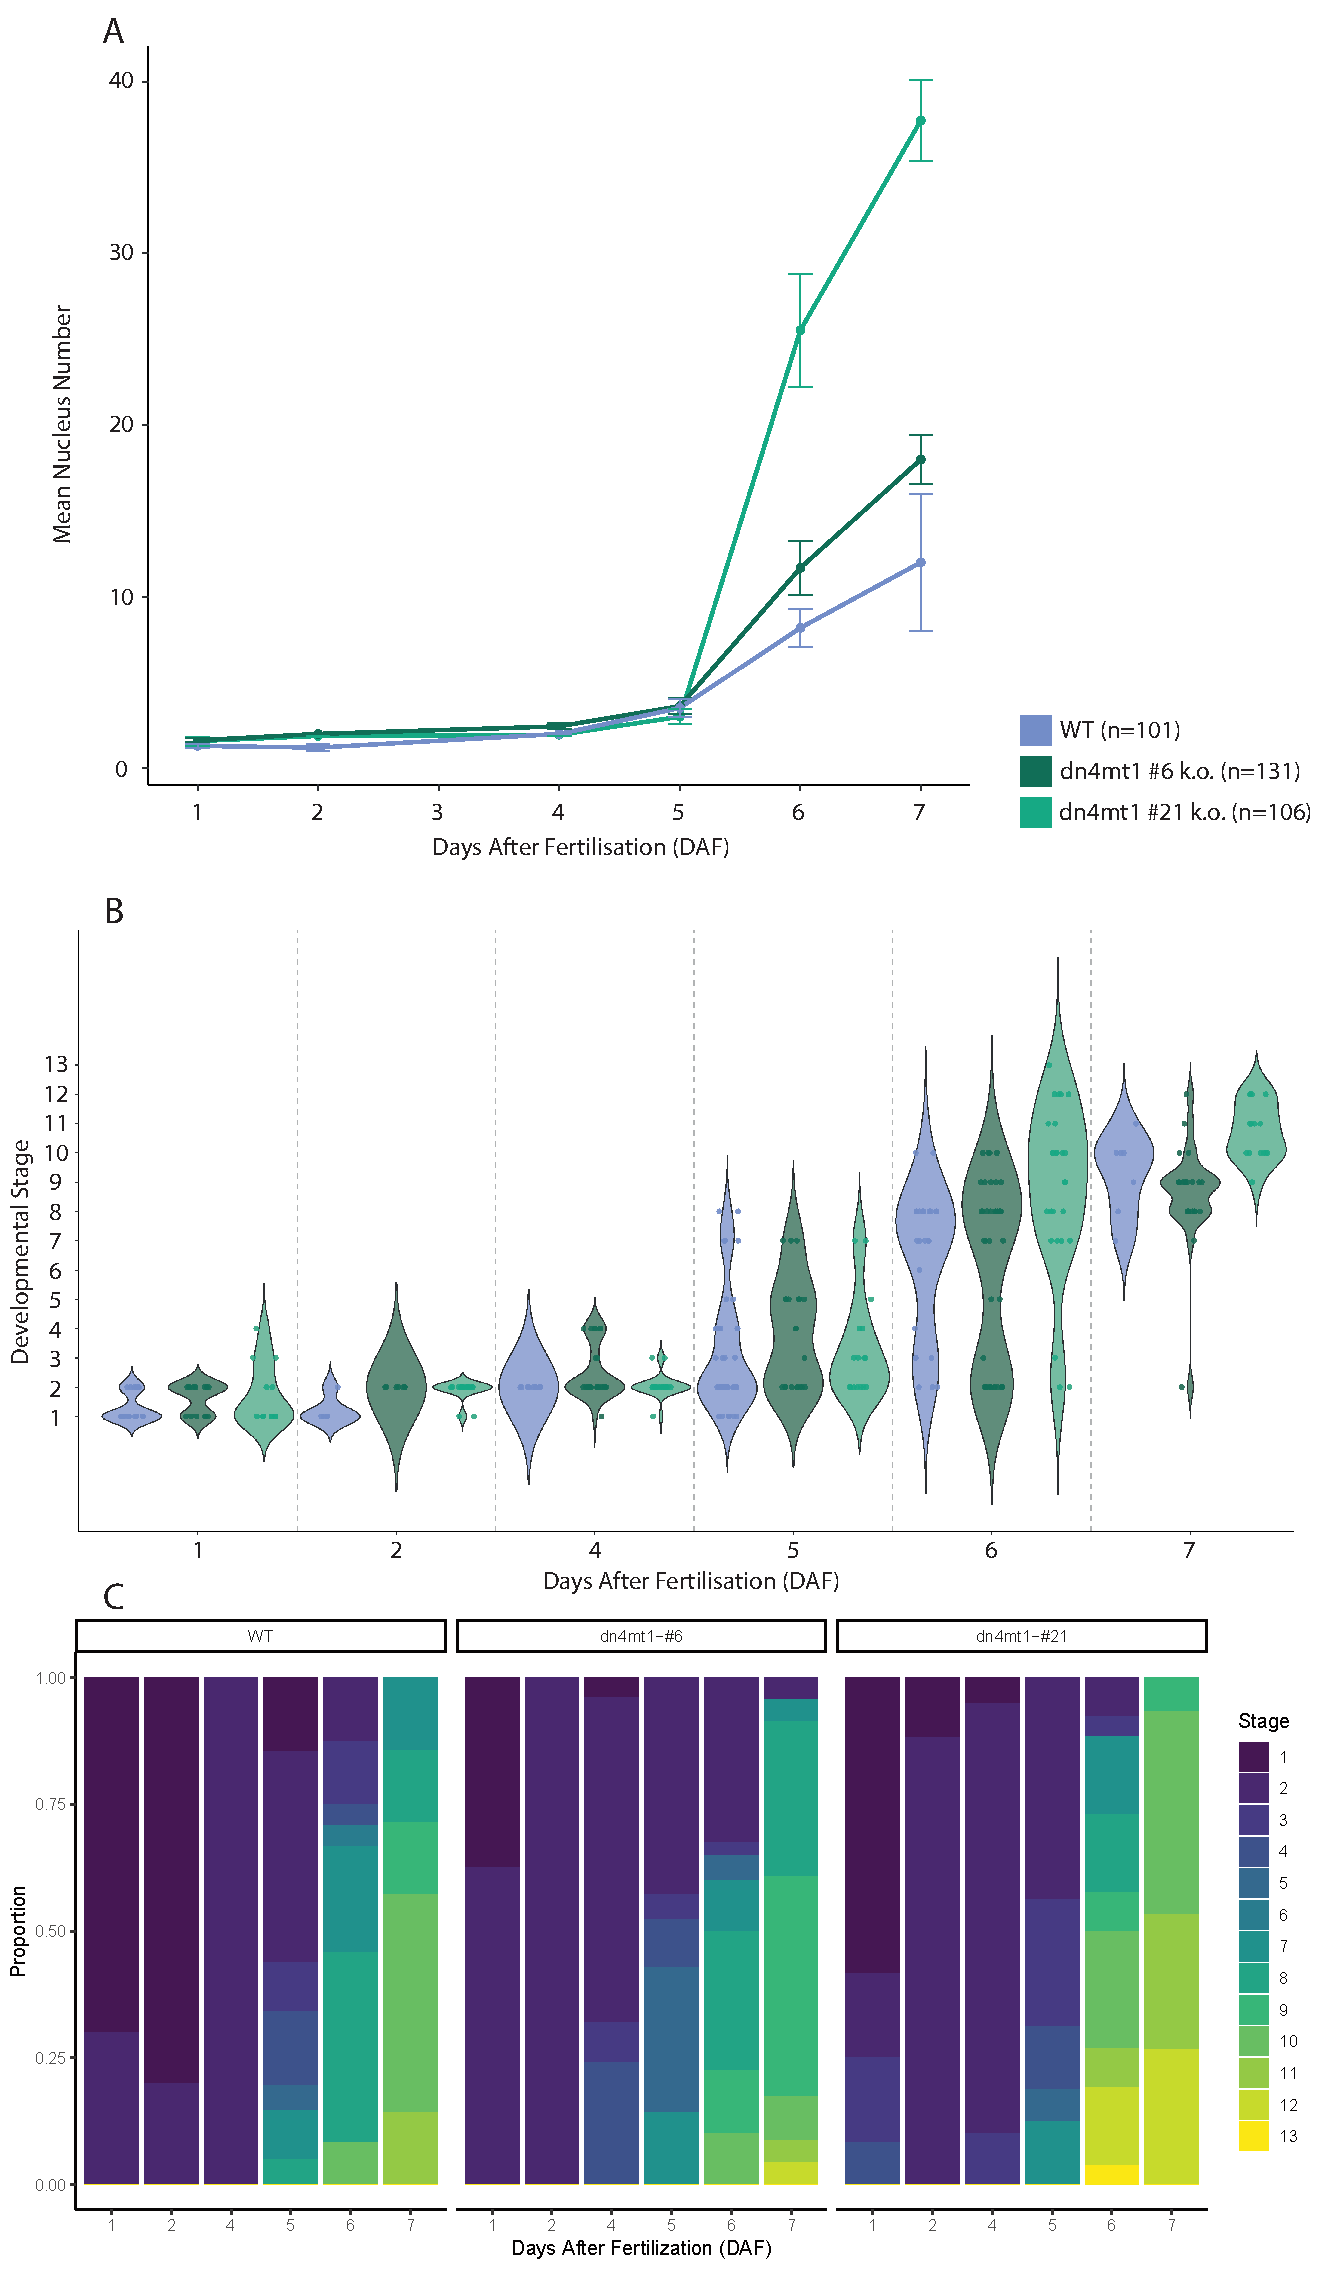
\includegraphics[width=0.95\textwidth]{Chapter3/Figs/Figure11_nucleus_number.pdf}
    \captionsetup{belowskip=0pt, aboveskip=0pt}
    \caption{\textbf{Embryos fertilised by \textit{dn4mt1} knockout sperm develop more rapidly than WT}}
    \label{fig:nucleus_number}
    \caption*{See next page for full caption.}
\end{figure}

\clearpage 

\FloatBarrier  % Prevents floating content from passing this point

% Full caption on the next page
\noindent\textbf{Full caption for Figure \ref{fig:nucleus_number}:} \\
A) Mean nucleus number of embryos from 1-7 days after fertilisation, fertilised by wild type (blue), \textit{dn4mt1} knockout \#6 (dark green), or \textit{dn4mt1} knockout \#21 (light green) sperm. 
B) Distribution of imaged embryos in different developmental stages from 1-7 days after fertilisation, categorised into distinct stages based on nuclei and cell numbers. 
Developmental stages: 1. 1 nucleus 2. 2 nuclei, 1 cell, 3. 2 nuclei, 2 cells 4. 4 nuclei, 2 cells, 5. 4 nuclei, 4 cells, 6. 8 nuclei, 4 cells, 7. 8 nuclei, 8 cells, 8. 9-16 nuclei, 9. 16-25 nuclei, 10. 26-35 nuclei, 11. 36-45 nuclei, 12. 46 - 55 nuclei, 13. 55< nuclei.
C) Proportion of embryos in developmental stages 1-7 days after fertilisation fertilised by wild type, \textit{dn4mt1} knockout \#6, or \textit{dn4mt1} knockout \#21 sperm.


\clearpage


\section{Discussion}


In angiosperms and other land plants, spermiogenesis involves chromatin compaction through the replacement of histones with sperm-specific histone variants \citep{RN283,RN284,RN285}. However, in \textit{Marchantia}, this process differs, as nucleosomes are replaced by protamines rather than histone variants. Consequently, DNA methylation becomes the primary heritable epigenetic mark in the paternal genome. This resembles the process in mammalian sperm, where the majority of histones are replaced by protamines, although some nucleosomes are retained \citep{RN282}. Following fertilisation, mammalian zygotes undergo global DNA demethylation, driven by TET enzymes. This demethylation is crucial for transcriptional regulation, imprinting, and maintaining pluripotency in the early stages of development \citep{RN286,RN287}.

In \textit{Marchantia}, following fertilisation, protamines in the paternal pronucleus are replaced by histones, and H3K27me3 is deposited by a maternally expressed PRC2 complex \citep{RN160} specifically on paternal chromatin. This suggests a potential mechanism for paternal genome recognition, with paternal N4-methylcytosine blanket methylation emerging as a potential candidate.

However, when examining the distribution of H3K27me3 marks over genes and transposons, there is no clear alignment with 4mC occupancy (Figure \ref{fig:h3k27me3}). Furthermore, results from scBS-seq of early Marchantia embryos revealed no evidence of paternal 4mC (Figure \ref{fig:ends_analysis}, Table \ref{tab:methylation_levels}). Additionally, Dr. Shujuan Xu confirmed that paternal H3K27me3 foci still form in embryos fertilised by \textit{dn4mt1} knockout sperm, 13 days after fertilisation (Figure \ref{fig:immuno}. These findings suggest that paternal genome recognition is not directly linked to blanket genome-wide 4mC methylation. However, it is important to consider that theoretical paternal 4mC trace levels in the embryo would likely be very low by 7-8 days post-fertilisation, assuming passive loss through cell division (Table \ref{tab:methylation_levels}). To obtain a definitive answer,  developing reliable 4mC immunostaining and/or single-cell AMD sequencing methods for zygotes or embryos at the 2-4 cell stage is essential, provided successful dissection at this early developmental stage can be achieved.

 Considering the shut-down of the paternal genome in the sporophyte, the possibility of whether sRNA production from the paternal genome became an intriguing question. Investigating whether there is a difference in sRNA production between the two parental genomes in the sporophyte, particularly in light of this potential suppression, revealed intriguing results. Initially, the sRNA data suggested a paternal bias in the embryo, which appeared to shift toward a maternal bias in the sporophyte, though substantial sRNA production was observed from both parental genomes (Figure \ref{fig:sRNA_SNPs}A,B). 
 
 Despite these findings, it is essential to acknowledge the limitations of this analysis. The male and female accessions used as the parental lines (Tak-1 and Tak-2) are asexually maintained in lab conditions, which means accumulated point mutations over time may significantly alter their genomic sequences. Indeed, at several SNP positions, bases other than the reference or alternative were observed across all datasets. Additionally, if Tak-1 had been crossed with other lines at any point, the resulting hybrid would exhibit a different SNP distribution from either parent.The unequal SNP distribution along different chromosomes further complicates the analysis, making these cultivars less suitable for complete genome coverage (Figure \ref{fig:chrom_ridge}). Moreover, the filtering steps applied to the sRNA data resulted in a limited number of data points, which restricts the ability to draw definitive conclusions. Ensuring the precise genetic background of the parental lines is therefore essential for accurate results, as is obtaining sufficient sequencing depths to definitively answer whether 24nt sRNAs are produced from both parental genomes in \textit{Marchantia} embryos. 
 
 Furthermore, exploring the distribution of H3K9me1 histone modifications on TEs in the mature embryo (as a proxy for locations that may be active in RdDM, as H3K9me2 has a direct interaction with SHH1, which recruits the Pol IV complex in \textit{Arabidopsis} \citep{RN116}) does not reveal a strong parental bias (Figure \ref{fig:h3k8me1}) \citep{RN160}. Nevertheless, addressing the limitations of the current dataset and producing a high-confidence, genetically distinct parental cross would provide valuable insights into the sRNA landscape of Marchantia embryos. These results could then be cross-referenced with bisulfite sequencing data to draw more robust conclusions.

It has been previously noted that similar to genes hypermethylated in the male germline of \textit{Arabidopsis} (MetGenes), \textit{de novo} methylated genes are also present in the sporophyte of \textit{Marchantia} (Figure \ref{fig:SLM_examples} \citep{jimmythesis}. In \textit{Arabidopsis}, few perfectly matching sRNAs map directly to methylated MetGene regions. This observation led to the discovery that HyperTE-derived sRNAs target MetGene locations in meiocytes for methylation with up to three mismatches \citep{RN187} (Figure \ref{fig:At_0v3}). 

Building on this, once MetGene loci were identified in \textit{Marchantia} sporophytes, it was explored whether CHH methylation  at these genes could be targeted by sRNAs produced by TEs with high sequence homology. Although sequence homology between TE sources and target MetGenes was identified (Figure \ref{fig:TE_SLM_pairs}), a clear relationship between sRNA mismatch targeting and CHH methylation was not established. Mapping sRNAs to MetGene locations with up to 3 mismatches did not significantly increase the abundance of sRNAs at these locations (Figure \ref{fig:Mp_0v3}). 

Nevertheless, a mechanism must allow either the production of 24nt sRNAs and/or the targeting of TE-derived sRNAs for methylation at MetGenes specifically during the sporophyte stage. Further investigation is needed to verify this hypothetical causal relationship, including examining RdDM-associated protein variants uniquely expressed in the sporophyte and/or creating CRISPR/Cas9 knockout lines to mutate homologous sequences from the putative TE source to determine whether CHH methylation is abolished at the corresponding MetGene.

 Previous studies have shown that the mature pre-meiotic embryo loses all traces of paternal 4mC methylation \citep{RN189}. The removal of 4mC may be necessary for embryo development, as there is evidence that 4mC suppresses chromatin accessibility and transcription \citep{RN189}. There are two possible pathways through which paternal blanket 4mC methylation could be absent in the mature embryo or sporophyte.  One possibility is that after fertilisation, MpDN4MT1 is not expressed, or 4mC methylation is not actively maintained, leading to its gradual dilution through cell division. Alternatively, we can hypothesise that paternal 4mC methylation needs to be removed to allow pronuclear fusion. This hypothesis could explain the unusually long period required for \textit{Marchantia} embryos to undergo pronuclear fusion and complete the first zygotic division (up to 3-4 days after fertilisation) \citep{RN139}. Additionally, the accelerated sporophyte maturation observed in embryos fertilised by \textit{dn4mt1} mutant sperm, maturing up to 4 days earlier than wild-type embryos (Figure \ref{fig:burstpeak}), could support this explanation. In this scenario, MpROS1X (a DNA glycosylase encoded on the female chromosome) emerges as a potential candidate that could facilitate the removal of paternal blanket 4mC prior to pronuclear fusion.

When comparing early embryonic development between the two 4mC mutants and wild type, it is evident that zygotic divisions began earlier in both 4mC mutants than in the wild type (Figure \ref{fig:nucleus_number}B,C). Following this initial difference, all genotypes developed at a similar rate until day 5, with comparable nucleus numbers. However, after day 5, the 4mC mutants exhibited a sharp exponential increase in cell numbers over the next two days, while wild type embryos also underwent rapid cell division, but with a more gradual increase (Figure \ref{fig:nucleus_number}). Interestingly, despite the expectation that the wild type embryo's delayed early embryonic development would lead to a delayed entry into exponential growth compared to the 4mC mutants, both genotypes entered this phase simultaneously. The primary difference lay in the rate of cell proliferation, rather than the timing of its onset.

These findings suggest that 4mC removal may be required prior to pronuclear fusion. However, more detailed immunostaining or single-cell AMD sequencing in the zygote is necessary, along with an investigation into the phenotypic effects of knocking out DNA demethylases, particularly MpROS1x. Additionally, it would be important to explore whether ROS1x possesses N4-methylcytosine glycosylase activity. Furthermore, despite accelerated embryonic development, the knockout of paternal 4mC appears to have a partial fertility cost, as some embryos in these knockouts exhibit delayed development or arrest (Figure \ref{fig:nucleus_number}B,C), a phenomenon observed in previous studies \citep{RN189}.

\clearpage

\section{Materials and Methods}

\subsection{Plant materials and growth conditions}

Male and female \textit{Marchantia polymorpha, L.} subsp. \textit{rudealis} accessions Takaragaike-1 (Tak-1, male) Takaragaike-2 (Tak-2, female) and Cam-2 (female) was used. The plants were grown on 1\% agar (Sigma-Aldrich), supplemented with ½ strength Gamborg's B5 medium. They were grown in a controlled environment chamber (Conviron) at 21°C with 70\% humidity under constant light with far-red light for induction of sexual reproduction, as described previously \citep{RN212,RN254}.

\subsection{Plasmid construction}

Four constructs were generated in total  using a Gateway\textregistered cloning system with either constitutive promoter 35S or the endogenous promoter EF$\alpha$, driving either citrine or tdTomato fluorophores with a nuclear localisation signal (NLS).

The insert for the BP reaction was amplified from plasmids pMpGWB115 (plasmid \#68569, Addgene) and pMpGWB116 (plasmid \#68570, Addgene) \citep{RN72} to get the citrine-NLS and tdTomato-NLS fragments respectively. The BP reactions were performed using the donor plasmid pDONR\texttrademark221 (Thermo Fisher (Invitrogen)). The LR reactions were performed using plasmids pMpGWB102 (plasmid \#68556, Addgene) and pMpGWB103 (plasmid \#68557, Addgene)\citep{RN72} as the backbones for the 35S and EF$\alpha$ promoter driven expression clones respectively. These constructs yielded the final 4 expression clones: MpGWB102(p35S)-citrine-NLS, MpGWB102(p35S)-tdTomato-NLS, MpGWB103(pEF$\alpha$)-citrine-NLS, MpGWB103(pEF$\alpha$)-tdTomato-NLS. The constructs were transformed into \textit{Escherichia  coli}, purified and the sequence confirmed, followed by transformation into \textit{Agrobacterium tumefaciens} strain MP90.

The primers used and plasmid maps are available in Appendix B Table \ref{table:reporter_primers} and Figures \ref{fig:35S_citrine_map}, \ref{fig:35S_tdTomato_map}, \ref{fig:EFalpha_citrine_map} and \ref{fig:EFalpha_tdTomato_map}.

\subsection{Thallus and sporeling transformation}

For thallus transformation, Tak-1 gemmae were grown for 18-20 days in a controlled environment chamber (Conviron) at 21°C with 70\% humidity under constant light on 1.2\% agar (Sigma-Aldrich), supplemented with ½ strength Gamborg's B5 medium. Following 18-20 days, thalli were cut and the basal fragments regenerated on plates supplemented with 1\% sucrose for 3 days. THe thalli were then co-cultured with Agrobacteria (strain MP90) in 0M51C liquid media for 3 days and transformants selected on 1\% agar (Sigma-Aldrich) supplemented with 10 $\mu$g/mL hygromycin and 120 $\mu$g/mL cefotaxime for several weeks. Fluorescent gemmae were selected from transformant thalli and regenerated again to avoid chimeric plants\citep{RN147}. 

For sporeling transformation, sporangia of backgrounds WT x WT, WT x Mp\textit{dn4mt1} \#6 and T x Mp\textit{dn4mt1} \#21 were sterilised in 1mL of Milton's sterilising solution on a rotating shaker for 20 minutes. The spores were pelleted and washed with sterile water twice. The sterilised spore suspension was added into 25mL 0M51C liquid medium and the flasks were incubated in a growth chamber with constant light at 1500-2000 lux, 23 °C for 5-7 days. Induced Agrobacterial cultures (strain MP90) containing each vector was co-cultivated with the sporelings for 2 days on a rotating shaker. the spore culture was strained and washed with sterile water and transformants were selected on 1\% agar (Sigma-Aldrich) supplemented with 10 $\mu$g/mL hygromycin and 120 $\mu$g/mL cefotaxime for several weeks\citep{RN146}.

\subsection{Semi in vitro culture and crossing}

Semi in vitro culture and crossing was performed as described previously\citep{RN139}. Briefly, mature female archegonia were collected into 5mL tubes containing 3mL water and co-cultured with male antheridia for 1 hour under white light at 22°C. The fertilised archegonia were then washed and incubated in 5mL tubes containing 3mL of fresh water under white light at 22°C until observation.

\subsection{Microscopy} 

The archegoniophores were collected for dissection and imaging and were either observed live or were fixed for imaging. For live cell imaging, rows of archegonia were manually dissected from the base of digitate rays and the embryo dissected out using micro knives or double lancet sapphire surgical knives (Fine Science Tools, World Precision Instruments) collected on cavity slides (BRAND\textregistered) and washed twice with 1x PBS to remove any maternal tissue. They were then stained with DAPI for 5 mins and briefly vacuum infiltrated and observed using slides with imaging spacers (Thermo Scientific™ Gene Frame) or on cavity slides \citep{RN139}. 

For observing developmental synchronicity and the Mp\textit{dn4mt1} early developmental phenotype,  rows of archegonia were manually dissected from the base of digitate rays removing involucres. The fluorescent samples were fixed and stained using the iTOMEI protocol \citep{RN148} using 1\% FA fixation for an hour in 1X PBS (pH 7.4) followed by clearning (20\% caprylyl sulfobetaine for 24 hours) and mounted in iohexol with imaging spacers (Thermo Scientific™ Gene Frame). The embryo/egg cells were imaged using a Leica SP8X confocal microscope.

\subsection{AMD-sequencing and bisulfite-sequencing library construction}

Dissected Tak-1 x Cam-2 embryos were used to construct 4mC-AMD-seq libraries using the xGen™ Methyl-Sequencing DNA Library Preparation Kit (IDT, 10009860) after treatment of sheared DNA with APOBEC3A (NEB \#E7120S), following manufacturer’s instructions. In parallel, a bisulfite sequencing library was also contructed after APOBEC3A treatment using the Imprint\textregistered DNA Modification Kit (Sigma-Aldrich, MOD50)


\subsection{Imaging analysis}

The collected images were analysed in Fiji (ImageJ) \citep{RN266}. The macro was created to automate the image analysis steps, whereby a maximum Z projection was applied to the 3D image stack and a Gaussian blur was applied. The selected region on interest (the embryo) was then masked and a local contrast was then enhanced using the CLAHE plugin, and nuclei were counted manually in the resulting images using the ROI Manager. The resulting data was visualised in R using the ggplot2 package.

\subsection{Determination of MetGenes}

MetGene locations were defined using parameters previously described \citep{jimmythesis}. Briefly, bisulfite sequencing reads were mapped using a custom mapping script based on Bismark \citep{RN229}, and fractional methylation (50bp windows) was determined for each sample in the  CG, CHG and CHH contexts using MethylDackel v0.4.0 and custom scripts. Windows were selected where C-methylation was greater than 0.05 and adjacent windows merged if they occured within 200bp. The methylation difference in each context was determined between the sporophyte and thallus, and retained according to these filtering criteria: Islands greater than 99bp; significantly different non-CG metylation between sporophyte and thallus (Fisher's exact test p<0.001); CG, CHG, CHH and non-CG difference between sporophyte and thallus bigger than 0, 0.05, 0.1 and 0.3 respectively. The final filtering step kept islands that had less than 0.1 CG methylation in the thallus and overlapped genic regions. The final list yielded 221 DMRs.

\subsection{Histone analysis}

CUT\&RUN reads were were processed using SAMtools v1.9 \citep{RN174}, BEDtools v2.27.1 \citep{RN90} and Picard v2.18.27 \citep{RN173} then mapped to the Takv6.1 genome \citep{RN179} using bwa v0.7.17 \citep{RN182}. To distinguish between maternal and paternal sequencing reads, a SNP analysis was conducted. SNPs were called using gatk v4.0.1.2 \citep{RN177} wherein the SNPs between the parental Tak-1 and Cam-2 were replaced with Ns. The parental reads were assigned using SNPSplit v0.3.4 \citep{RN178} and counts for each parental genome were calculated using SAMtools v1.9 and BEDTools v2.27.1. Please see reference \cite{RN160}  for a detailed description of the pipeline. 

\subsection{sRNA analysis}

The sRNA reads were processed using Trim Galore! v0.4.2 \citep{trim_galore}, and mapped using bowtie v1.0.1 \citep{RN89} allowing for 0 or up to 3 mismatches with the -v option. For the TE-MetGene matching analysis, the resulting BAM files were converted to fasta files using custom awk scripts. The reads were once again mapped using bowtie, with no mismatches. Finally the resulting reads in the BAM files were queried against original genome locations using custom awk scripts, and the resulting file was filtered by MetGene locations with BEDtools v2.27.0.

For the sRNA SNP analysis, a SNP file was created using the method described above but this time using Tak-1 and Tak-2 as the parental genomes. 24nt reads overlapping MetGene locations with 0 or 1 mismatches were filtered using BEDtools v2.27.0 and were kept if they overlapped SNP positions. From the 1 mismatches dataset, only reads that mismatched exactly at the SNP positions were kept to prevent reads that mismatch elsewhere but also covering SNP positions from biasing the data. The perfect matching dataset was downsampled to prevent this much larger dataset from biasing the data. The reference, alternative or other bases were counted at each SNP position using SAMtools mpileup and this dataset was imported to R for visualisation in R using the ggplot, ggpubr and ggridges packages. Please find all scripts used at \href{https://github.com/talasjudit}{my personal GitHub page}.



%!TEX root = ../thesis.tex
%*******************************************************************************
%****************************** Fourth Chapter **********************************
%*******************************************************************************
\chapter{Main Discussion}

% **************************** Define Graphics Path **************************
\ifpdf
    \graphicspath{{Chapter4/Figs/}}
\else
    \graphicspath{{Chapter3/Figs/}}
\fi


This thesis aimed to investigate the epigenetic mechanisms regulating gene expression and genome stability during plant reproduction, focusing on two plant systems: \textit{Arabidopsis thaliana} and \textit{Marchantia polymorpha}. Specifically, I examined the expression patterns of key RNA-directed DNA methylation (RdDM) components in \textit{Arabidopsis} the development of the male sexual lineage, described the 24nt sRNA profiles after meiosis in microspores and sperm. I also explored the dynamics of DNA methylation, particularly the inheritance of the paternal epigenetic mark N4-methylcytosine (4mC), during early embryo development in \textit{Marchantia}. To address these aims, I employed a combination of small RNA sequencing, bisulfite and APOBEC3A-mediated methylation sequencing,  fluorescent reporter line construction and imaging and developing bioinformatics pipelines and data analysis of novel and existing data. The findings reveal novel insights into the epigenetic regulation of plant reproduction and highlight the diverse mechanisms employed by different plant lineages.

\section{Tissue-Specific Regulation of RdDM}

The analysis of NRPD1 and NRPE1 expression patterns in Arabidopsis revealed a dynamic regulation of these key RdDM components during pollen development. NRPD1, the largest subunit of RNA Polymerase IV, showed confined expression in the tapetal layer and surrounding somatic anther tissue during the meiocyte stage, with subsequent expression in microspores but absence in mature pollen. In contrast, NRPE1, the largest subunit of RNA Polymerase V, exhibited broader expression in both somatic and germline tissues throughout anther development. 

Investigation of CLSY chromatin remodeler expression in anthers provided further insights into RdDM regulation. CLSY3 expression was confirmed to be confined to the tapetum and absent in later developmental stages. Similarly, CLSY1 and CLSY2 were not detected in maturing pollen. However, some discrepancies were noted when these findings were cross-referenced with RNA-sequencing data. Despite these ambiguities, the sRNA profiles largely corroborated the observed expression patterns of CLSY proteins. This suggests a potential shift in the regulation of sRNA production after meiosis, possibly involving alternative mechanisms for small RNA biogenesis and highlighting the importance of non-canonical RdDM pathways in the male sexual lineage.

These findings collectively indicate a complex temporal and spatial regulation of the RdDM pathway during the development of the male sexual lineage, with potential implications for the establishment and maintenance of DNA methylation patterns. The observed changes in CLSY expression patterns may reflect the dynamic nature of epigenetic regulation during pollen development and highlight the need for further investigation into the mechanisms governing sRNA production in mature pollen.

\section{Sperm cell-specific small RNA clusters are uncoupled from CLSY-dependent loci}

The analysis of small RNA profiles in Arabidopsis sperm cells revealed a unique landscape distinct from both earlier germline stages and somatic tissues. Firstly, a family of LTR/Gypsy TEs was identified as producing sperm-specific 24nt sRNAs which may hint at ATGP2N reactivation in the sperm cell, or the 24nt sRNAs may originate from the vegetative cell based on CHH profiles. Secondly, around 20\% of MetGenes produce 24nt sRNAs specifically in the sperm cell, including genes important in mediating CG methylation. Finally, while CLSY1 and CLSY2-dependent loci produce abundant sRNAs in somatic tissues, sperm cells exhibit a different pattern. Many sperm-specific small RNA clusters do not overlap with known CLSY-dependent loci, further hinting at the involvement of non-canonical RdDM pathways in the biogenesis or sRNAs in this tissue. These findings indicates a shift in the regulation of epigenetic pathways during the final stages of the development of the male sexual lineage, which may be crucial for genome integrity. 

\section{A novel dissection and sequencing protocol showed that paternal 4mC is lost in early \textit{Marchantia} embryos and that the knockout of paternal 4mC results in accelerated early embryonic development}

A novel method of dissecting early \textit{Marchantia} embryos was trialled and perfected, allowing the successful trial of low input AMD and bisulfite sequencing protocols. Furthermore, a fixing and clearing protocol was optimised to explore early embryonic development in Marchantia. Nuclear reporter lines of wild type male, female and \textit{dn4mt1} male \textit{Marchantia} plants were constructed screened and used to study the effect of 4mC knockouts in early embryonic development.

I presented evidence that  paternal 4mC methylation, which is deposited during spermiogenesis, is lost in the early embryo. Our analysis of early embryos (7-8 days after fertilisation) showed no detectable levels of 4mC methylation. This, together with the accelerated developmental phenotype of embryos fertilised by \textit{dn4mt1} mutant sperm hints at the requirement of 4mC removal prior to pronuclear fusion.

Our live cell imaging experiments revealed that embryos fertilised by sperm lacking 4mC methylation (dn4mt1 mutants) initiate cell division earlier and develop more rapidly during the first 7 days post-fertilization compared to wild-type embryos. This finding provides insight into the functional significance of 4mC in regulating the timing of early embryonic events in Marchantia.

\section{Sporophyte-specific genic methylation is likely targeted by RdDM and a novel method for assigning reads from parental origins for sRNA data is developed}

Regions with \textit{de novo} genic methylation in the sporophyte of \textit{Marchantia} were identified and their relationship with TE-derived sRNA clusters was explored. While sequence homology between TEs and MetGenes was identified, no clear relationship was established between sRNA mismatch targeting and increased CHH methylation at MetGenes. Mapping sRNAs with up to three mismatches did not result in a significant increase in sRNA abundance at these MetGene loci.

The study also explored the potential differences in sRNA production between the paternal and maternal genomes in the sporophyte, especially given the shutdown of the paternal genome. Initial data suggested a paternal bias in sRNA production during the embryo stage, which shifted towards a maternal bias in the sporophyte, although both parental genomes continued to produce substantial amounts of sRNAs.

\section{Future Directions}

Investigating the mechanisms of paternal 4mC removal in Marchantia
While we have observed the rapid loss of paternal 4mC in early Marchantia embryos, the exact mechanism remains unclear. Future research should focus on determining whether this loss occurs through passive dilution or active removal. Developing single-cell AMD sequencing methods for zygotes or 2-4 cell stage embryos would provide valuable insights into the dynamics of 4mC loss. Additionally, investigating the potential role of DNA demethylases, particularly MpROS1x, in active 4mC removal would be crucial. Functional studies of MpROS1x, including its potential N4-methylcytosine glycosylase activity, could shed light on the mechanisms of epigenetic reprogramming in early Marchantia embryos.

Understanding Cross-Cellular Communication
This thesis also raises important questions about the mechanisms underlying cross-cellular sRNA movement in reproductive tissues. While it is clear that plasmodesmata facilitate the transfer of sRNAs between the tapetum and germline cells, the exact molecular players involved in this process are still poorly understood. Future studies should focus on elucidating the pathways that regulate sRNA movement during germline development and their impact on epigenetic inheritance.

Investigating non-canonical RdDM pathways post-meiosis



Our discovery of unique small RNA clusters in Arabidopsis sperm cells that are uncoupled from known CLSY-dependent loci opens up new avenues for research. Future studies should aim to identify the mechanisms responsible for generating these sperm-specific small RNAs and their potential targets. Investigating the functional significance of these small RNAs in sperm cell development, fertilization, and early embryogenesis would provide valuable insights into male gamete-specific epigenetic regulation. This could involve generating mutants defective in sperm-specific small RNA production and analyzing their effects on fertility and early seed development.

The accelerated development observed in embryos fertilized by 4mC-deficient sperm suggests a regulatory role for this epigenetic mark in early embryogenesis. Future research should focus on elucidating the molecular mechanisms by which 4mC influences cell cycle progression and gene expression in early embryos. This could involve transcriptome analysis of wild-type and dn4mt1 mutant embryos at various early developmental stages, as well as identifying potential 4mC readers that may mediate its effects on embryonic development. Additionally, investigating the long-term consequences of accelerated early development on sporophyte growth and fitness would provide insights into the evolutionary significance of 4mC-mediated regulation.
 including examining RdDM-associated protein variants specific to the sporophyte and employing CRISPR/Cas9 to mutate homologous sequences from the potential TE sources. This would help determine whether CHH methylation at the corresponding MetGenes is abolished.

\section{Concluding remarks}
\chapter*{Glossary}
\addcontentsline{toc}{chapter}{Glossary}

\begin{description}[align=left, labelwidth=3cm]
    \item[4mC] N4-methylcytosine
    \item[5mC] 5-methylcytosine
    \item[AGO] ARGONAUTE
    \item[AMD-seq] APOBEC3A-mediated deamination sequencing
    \item[BS-seq] bisulfite sequencing
    \item[CLSY] CLASSY
    \item[CMT] CHROMOMETHYLASE
    \item[cRdDM] canonical RdDM
    \item[DAF] days after fertilisation
    \item[DME] DEMETER
    \item[DML] DEMETER-LIKE
    \item[DMS] DEFECTIVE IN MERISTEM SILENCING
    \item[DNA] deoxyribonucleic acid
    \item[DNMT] DECREASED DNA METHYLATION
    \item[DRD] DEFECTIVE IN RNA-DIRECTED DNA METHYLATION
    \item[DRM] DOMAINS REARRANGED METHYLTRANSFERASE
    \item[easiRNA] epigenetically active small interfering RNA
    \item[EF$\alpha$] elongation factor 1$\alpha$
    \item[EM-seq] Enzymatic methylation sequencing
    \item[FPKM] fragments per kilobase of transcript per million mapped reads
    \item[Gb] gigabases
    \item[gDNA] genomic DNA
    \item[KTF] KOW DOMAIN-CONTAINING TRANSCRIPTION FACTOR
    \item[LTR] long-terminal-repeat
    \item[Mb] megabases
    \item[MET1] METHYLTRANSFERASE 1
    \item[miRNA] micro RNA
    \item[MORC] MICRORCHIDIA
    \item[NERD] NEEDED FOR RDR2-INDEPENDENT DNA METHYLATION
    \item[NRPD] NUCLEAR RNA POLYMERASE D
    \item[NRPE] NUCLEAR RNA POLYMERASE E
    \item[nt] nucleotide
    \item[PGTS] post-transcriptional gene silencing
    \item[piRNA] PIWI-interacting small RNA
    \item[Pol IV] RNA Polymerase IV
    \item[Pol V] RNA Polymerase V
    \item[PTGS] post-transcriptional gene silencing
    \item[RdDM] RNA-directed DNA methylation
    \item[RDM1] RNA-DIRECTED DNA METHYLATION1
    \item[RDR] RNA-DEPENDENT RNA POLYMERASE
    \item[RNA] ribonucleic acid
    \item[ROS] REPRESSOR OF SILENCING
    \item[RPKM] reads per kilobase per million mapped reads
    \item[RPM] reads per million
    \item[SHH] SAWADEE HOMEODOMAIN HOMOLOGUE
    \item[SPT5L] SUPPRESSOR OF TY INSERTION 5 LIKE
    \item[sRNA] small RNA
    \item[siRNA] small interfering RNA
    \item[SUVH] SUPPRESSOR OF VARIEGATION 3–9 HOMOLOG
    \item[TE] transposable element
    \item[TET] Ten-eleven translocation
    \item[TGS] transcriptional gene silencing
    \item[TSS] transcriptional start site
    \item[tRFs] tRNA fragments
    \item[tRNA] transfer RNA
\end{description}



% ********************************** Back Matter *******************************
% Backmatter should be commented out, if you are using appendices after References
%\backmatter

% ********************************** Bibliography ******************************
\begin{spacing}{0.9}

% To use the conventional natbib style referencing
% Bibliography style previews: http://nodonn.tipido.net/bibstyle.php
% Reference styles: http://sites.stat.psu.edu/~surajit/present/bib.htm

%\bibliographystyle{apalike}
\bibliographystyle{unsrt} % Use for unsorted references  
%\bibliographystyle{plainnat} % use this to have URLs listed in References
\cleardoublepage
\bibliography{References/references} % Path to your References.bib file


% If you would like to use BibLaTeX for your references, pass `custombib' as
% an option in the document class. The location of 'reference.bib' should be
% specified in the preamble.tex file in the custombib section.
% Comment out the lines related to natbib above and uncomment the following line.

%\printbibliography[heading=bibintoc, title={References}]


\end{spacing}

% ********************************** Appendices ********************************

% Remove automatic "Appendix" prefix from chapter titles
\appendix
\renewcommand{\thechapter}{} % Prevent chapter numbering from showing automatically

\renewcommand{\thefigure}{A\arabic{figure}} % For figures in Appendix 1
\renewcommand{\thetable}{A\arabic{table}}   % For tables in Appendix 1
\setcounter{figure}{0} % Reset the figure counter
\setcounter{table}{0}  % Reset the table counter

\chapter*{\LARGE Appendix A - Chapter 2}
\addcontentsline{toc}{chapter}{Appendix A - Chapter 2} % Add to TOC manually
\label{appendix:chapter2}
%!TEX root = ../thesis.tex
% ******************************* Thesis Appendix A ****************************


%\begin{verbatim}
%mount -t iso9660 -o ro,loop,noauto /your/texlive####.iso /mnt
%\end{verbatim}


\renewcommand{\thefigure}{B\arabic{figure}} % For figures in Appendix 2
\renewcommand{\thetable}{B\arabic{table}}   % For tables in Appendix 2
\setcounter{figure}{0} % Reset the figure counter
\setcounter{table}{0}  % Reset the table counter

\chapter*{\LARGE Appendix B - Chapter 3}
\addcontentsline{toc}{chapter}{Appendix B - Chapter 3} % Add to TOC manually
\label{appendix:chapter3}
%!TEX root = ../thesis.tex
% ******************************* Thesis Appendix B ********************************

\begin{figure}[htbp!] 
\centering    
    \includegraphics[width=1\textwidth]{Chapter3/Figs/Supps/FigureS1_Differences_in_development_embryos.pdf}
\caption{\textbf{\textit{Marchantia} embryos develop at different rates in different environmental conditions}}
\label{fig:embryo_diff}
\captionsetup{font=small}
    \caption*{DAPI stained \textit{Marchantia} embryos at 10 days after fertilisation (first row), and 12 days after fertilisation (second and third rows) showing different developmental stages. Scale bar 10 $\mu$m.}
\end{figure}

\begin{figure}[htbp!] 
\centering    
    \includegraphics[width=1\textwidth]{Chapter3/Figs/Supps/FigureS2_Fixing_MpSUN_trials.pdf}
\caption{\textbf{Fixing and staining of wild type (first row) ECPro::MpSUN-GFP embryos (third row) and gemmae (second row). Scale bar 10 $\mu$m.}}
\label{fig:MpSUN}
\captionsetup{font=small}
    \caption*{}
\end{figure}

\begin{figure}[htbp!] 
\centering    
    \includegraphics[width=1\textwidth]{Chapter3/Figs/Supps/FigureS3_enzyme_tests.pdf}
\caption{\textbf{Fixing and staining embryos after treatment with cell wall digesting enzymes}}
\label{fig:enzyme_tests}
\captionsetup{font=small}
    \caption*{Scale bar 10 $\mu$m.}
\end{figure}

\begin{figure}[htbp!] 
\centering    
    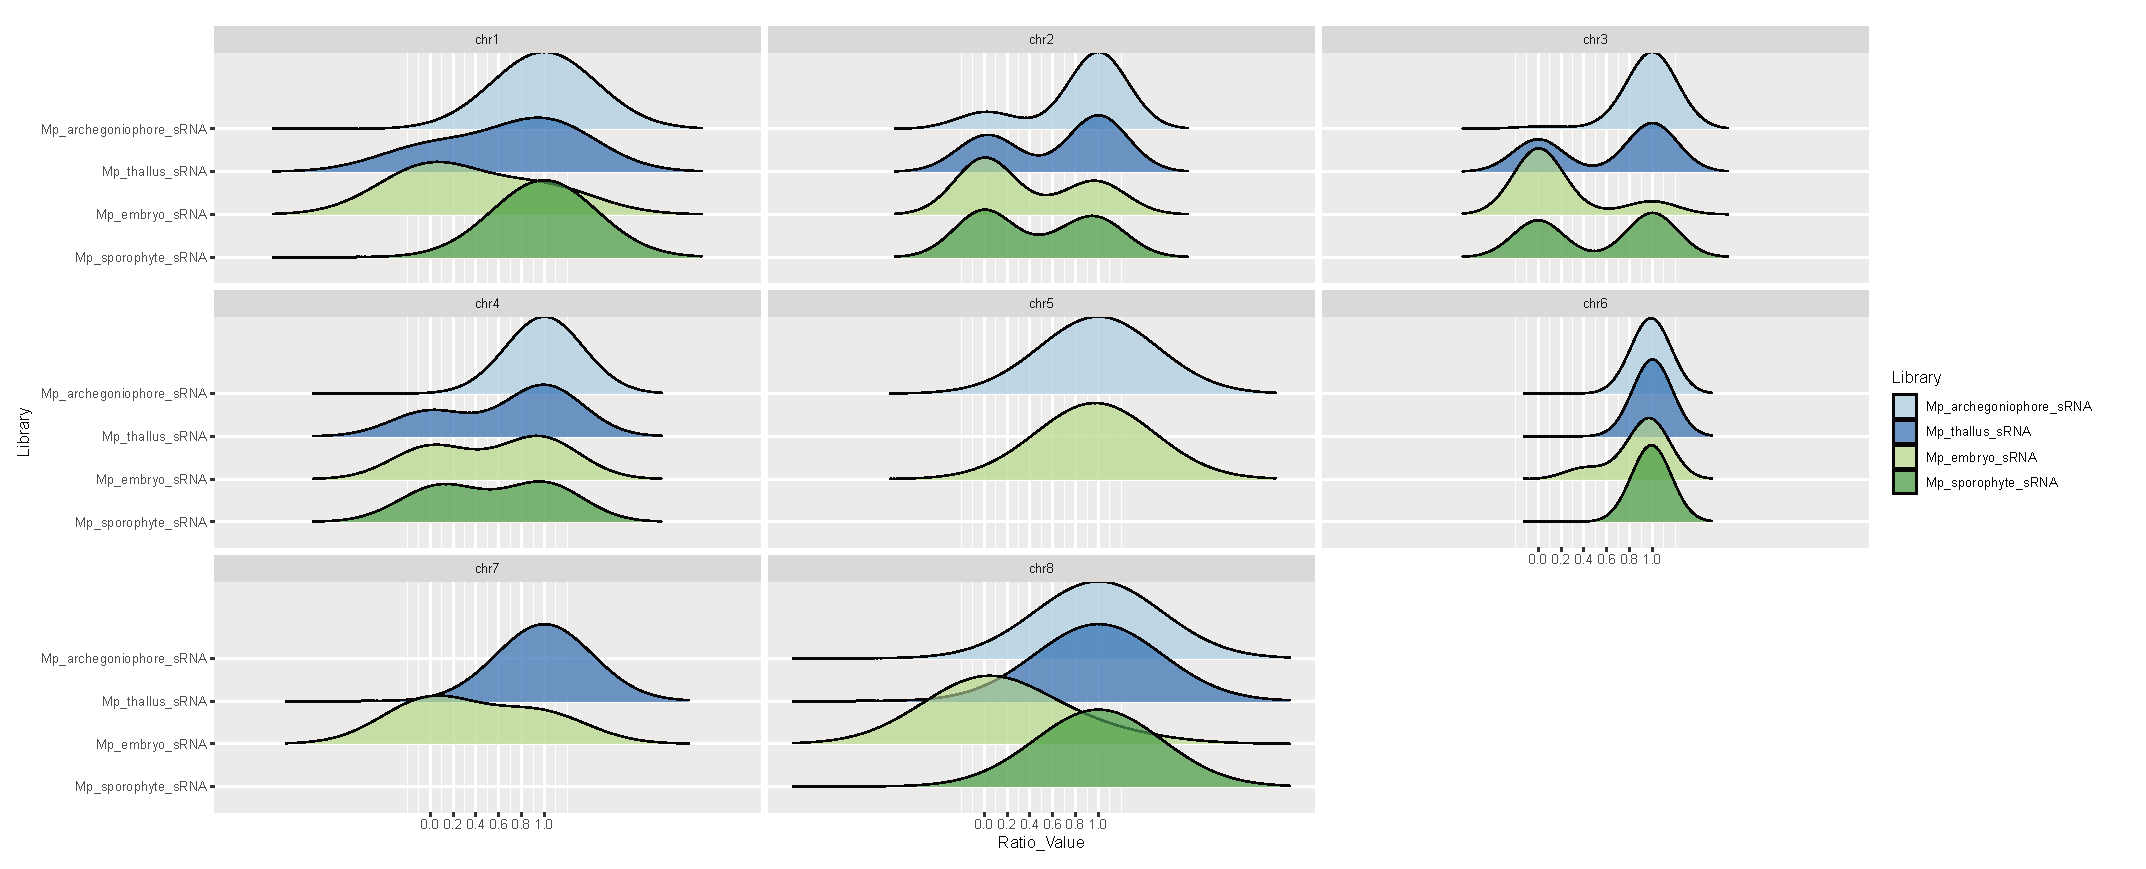
\includegraphics[width=1\textwidth]{Chapter3/Figs/Supps/FigureS_chrom_ridge_plot.pdf}
\caption{\textbf{}}
\label{fig:chrom_ridge}
\captionsetup{font=small}
    \caption*{}
\end{figure}

\begin{figure}[htbp!] 
\centering    
    \includegraphics[width=1\textwidth]{Chapter3/Figs/Supps/FigureS4_transverse_diameter.pdf}
\caption{\textbf{4mC mutant embryos start dividing earlier than WT embryos}}
\label{fig:Dividing_cells}
\captionsetup{font=small}
    \caption*{Line graph that shows dividing cells in embryos fertilised by wild type (blue) or 2 independent 4mC mutant (green) sperm.}
\end{figure}

\begin{figure}[htbp!] 
\centering    
    \includegraphics[width=1\textwidth]{Chapter3/Figs/Supps/FigureS5_H3k9me1.pdf}
\caption{\textbf{H3K9me1 over genes and TEs is not associated with the paternal genome and tends maternal}}
\label{fig:h3k8me1}
\captionsetup{font=small}
    \caption*{}
\end{figure}

\begin{figure}[htbp!] 
\centering    
    \includegraphics[width=1\textwidth]{Chapter3/Figs/Supps/FigureS1_immunostaining.pdf}
\caption{\textbf{Immunostaining of H3K27me3 in 13 DAF embryos fertilised by wild type and dn4mt1 \#21 knockout sperm }}
\label{fig:immuno}
\captionsetup{font=small}
    \caption*{}
\end{figure}

\begin{table}[htbp]
    \centering
    \scriptsize % Keep the font size as scriptsize
    \caption{Primers used for nuclear reporter line cloning}
    \label{table:reporter_primers}
    \begin{tabular}{>{\raggedright\arraybackslash}p{3.4cm} >{\raggedright\arraybackslash}p{2.8cm} >{\raggedright\arraybackslash}p{4.7cm} >{\raggedright\arraybackslash}p{1.9cm}}
    \toprule
    Construct Target & Name & Sequence & Purpose \\
    \midrule
    pMpGWB115 or pMpGWB116 & attB1-fluo-NLS-attB2-f1 & \seqsplit{GGGGACAAGTTTGTACAAAAAAGCAGGCTTAATGGTGAGCAAGGGCGAG} & citrine/tdTom insert + attB sites \\
    pMpGWB115 or pMpGWB117 & attB1-fluo-NLS-attB2-r1 & \seqsplit{GGGGACCACTTTGTACAAGAAAGCTGGGTTCTATCCTCCAACCTTTCTCTTCTTCTTAGG} & citrine/tdTom insert + attB sites \\
    \midrule
    pMpGWB102-Citrine-NLS \& pMpGWB103-Citrine-NLS entry clones (pDONR221) & citrine-ent-seq-f1 & \seqsplit{TTAATGGTGAGCAAGGGC} & Entry clone sequencing \\
    & citrine-ent-seq-r1 & \seqsplit{TGGGTTCTATCCTCCAACC} & Entry clone sequencing \\
    pMpGWB102-tdTom-NLS \& pMpGWB103-tdTom-NLS entry clones (pDONR221) & tdTom-ent-seq-f1 & \seqsplit{AGGCTTAATGGTGAGCAAG} & Entry clone sequencing \\
    & tdTom-ent-seq-r1 & \seqsplit{GGGTTCTATCCTCCAACC} & Entry clone sequencing \\
    \midrule
    pMpGWB102-Citrine-NLS & 102-citrine-exp-seq-f1 & \seqsplit{TTGGAGAGAACACGGG} & Expression clone sequencing \\
    & 102-citrine-exp-seq-r1 & \seqsplit{CTGGGTTCTATCCTCCAAC} & Expression clone sequencing \\
    pMpGWB102-tdTom-NLS & 102-tdTom-exp-seq-f1 & \seqsplit{AGAGAACACGGGGGACTC} & Expression clone sequencing \\
    & 102-tdTom-exp-seq-r2 & \seqsplit{TCGGAGGAGGCGGTG} & Expression clone sequencing \\
    & 102-tdTom-exp-seq-r1 & \seqsplit{ACAAGAAAGCTGGGTTCTATCCTC} & Expression clone sequencing \\
    \midrule
    pMpGWB103-Citrine-NLS & 103-citrine-exp-seq-f1 & \seqsplit{CCTCGAGCGAGTGATTTTTTAGG} & Expression clone sequencing \\
    & 103-citrine-exp-seq-r1 & \seqsplit{GGGTTCTATCCTCCAACCTTTC} & Expression clone sequencing \\
    pMpGWB103-tdTom-NLS & 103-tdTom-exp-seq-f1 & \seqsplit{ATTTCGCTAATCATTCCCTAATTTC} & Expression clone sequencing \\
    & 103-tdTom-exp-seq-r2 & \seqsplit{CGGCCATGTTGTTGTC} & Expression clone sequencing \\
    & 103-tdTom-exp-seq-r1 & \seqsplit{AAGAAAGCTGGGTTCTATCC} & Expression clone sequencing \\
    \bottomrule
    \end{tabular}
\end{table}

\begin{figure}[htbp]
\centering
\includegraphics[width=1\textwidth]{Appendix2/Figs/1-expression-clone-pMpGWB102(35S)+citrine Map.pdf}
\caption{Plasmid map of pMpGWB102(35S)-citrine-NLS}
\label{fig:35S_citrine_map}
\end{figure}

\begin{figure}[htbp]
\centering
\includegraphics[width=1\textwidth]{Appendix2/Figs/2-expression-clone-pMpGWB102(35S)+tdTomato Map.pdf}
\caption{Plasmid map of pMpGWB102(35S)-tdTomato-NLS}
\label{fig:35S_tdTomato_map}
\end{figure}

\begin{figure}[htbp]
\centering
\includegraphics[width=1\textwidth]{Appendix2/Figs/3-expression-clone-pGWB103(EFalpha)+citrine Map.pdf}
\caption{Plasmid map of pMpGWB103(EF$\alpha$)-citrine-NLS}
\label{fig:EFalpha_citrine_map}
\end{figure}

\begin{figure}[htbp]
\centering
\includegraphics[width=1\textwidth]{Appendix2/Figs/4-expression-clone-pGWB103(EFalpha)+tdTomato Map.pdf}
\caption{Plasmid map of pMpGWB102(EF$\alpha$)-tdTomato-NLS}
\label{fig:EFalpha_tdTomato_map}
\end{figure}

\begin{table}[htbp]
\centering
\begin{tabular}{|p{6cm}|p{3cm}|p{4cm}|} % Same column widths as the second part
\hline
\textbf{Line name} &  & \textbf{Source} \\
\hline
Tak-1 & & Feng Lab \\
Tak-2 & & Feng Lab \\
Cam-2 & & Feng Lab \\
35s::tdTomato-NLS (Tak-1 male, WT female backgrounds) & & Feng Lab (JT) \\
EF$\alpha$::citrine-NLS (Tak-1 male, WT female backgrounds) & & Feng Lab (JT) \\
EF$\alpha$::tdTomato-NLS (Ta-k1 male, WT female backgrounds) & & Feng Lab (JT) \\
dn4mt1 ko \#6 & & Feng Lab \citep{RN189} \\
dn4mt1 ko \#21 & & Feng Lab \citep{RN189} \\
dnmt3b ko & & Feng Lab \citep{RN189} \\
cmta ko & & Feng Lab \citep{RN189} \\
\hline
\end{tabular}
\begin{tabular}{|p{6cm}|p{3cm}|p{4cm}|} % Now use 3 columns for the second part
\hline
\textbf{Library name} & \textbf{Library type} & \textbf{Source} \\
\hline
WT sperm & EM-seq & Feng Lab (JT) \\
WT sperm & AMD-seq & Feng Lab (JT) \\
WT sperm & AMD-seq & Feng Lab \\
dn4mt1 ko sperm & AMD-seq & Feng Lab \\
14 DAF embryo & AMD-seq & Feng Lab (JT) \\
7-8 DAF embryo & A3A-sc-BS-seq & Feng Lab (JT) \\
\hline
Archegoniophore & sRNA & \href{https://academic.oup.com/pcp/article/57/2/359/2460930}{OUP} \\
Embryo & sRNA & Feng Lab \\
Sporophyte & sRNA & Feng Lab \\
Thallus & sRNA & Feng Lab \\
\hline
Embryo & BS-seq & Feng Lab \\
Sporophyte & BS-seq & Feng Lab \\
Thallus & BS-seq & Feng Lab \\
\hline
\end{tabular}
\caption{Line names, library types, and sources.}
\end{table}




% *************************************** Index ********************************
\printthesisindex % If index is present

\end{document}
